\documentclass{article} % For LaTeX2e
\usepackage{iclr2021_conference,times}

% Optional math commands from https://github.com/goodfeli/dlbook_notation.
%%%%% NEW MATH DEFINITIONS %%%%%

\usepackage{amsmath,amsfonts,bm}

% Mark sections of captions for referring to divisions of figures
\newcommand{\figleft}{{\em (Left)}}
\newcommand{\figcenter}{{\em (Center)}}
\newcommand{\figright}{{\em (Right)}}
\newcommand{\figtop}{{\em (Top)}}
\newcommand{\figbottom}{{\em (Bottom)}}
\newcommand{\captiona}{{\em (a)}}
\newcommand{\captionb}{{\em (b)}}
\newcommand{\captionc}{{\em (c)}}
\newcommand{\captiond}{{\em (d)}}

% Highlight a newly defined term
\newcommand{\newterm}[1]{{\bf #1}}


% Figure reference, lower-case.
\def\figref#1{figure~\ref{#1}}
% Figure reference, capital. For start of sentence
\def\Figref#1{Figure~\ref{#1}}
\def\twofigref#1#2{figures \ref{#1} and \ref{#2}}
\def\quadfigref#1#2#3#4{figures \ref{#1}, \ref{#2}, \ref{#3} and \ref{#4}}
% Section reference, lower-case.
\def\secref#1{section~\ref{#1}}
% Section reference, capital.
\def\Secref#1{Section~\ref{#1}}
% Reference to two sections.
\def\twosecrefs#1#2{sections \ref{#1} and \ref{#2}}
% Reference to three sections.
\def\secrefs#1#2#3{sections \ref{#1}, \ref{#2} and \ref{#3}}
% Reference to an equation, lower-case.
\def\eqref#1{equation~\ref{#1}}
% Reference to an equation, upper case
\def\Eqref#1{Equation~\ref{#1}}
% A raw reference to an equation---avoid using if possible
\def\plaineqref#1{\ref{#1}}
% Reference to a chapter, lower-case.
\def\chapref#1{chapter~\ref{#1}}
% Reference to an equation, upper case.
\def\Chapref#1{Chapter~\ref{#1}}
% Reference to a range of chapters
\def\rangechapref#1#2{chapters\ref{#1}--\ref{#2}}
% Reference to an algorithm, lower-case.
\def\algref#1{algorithm~\ref{#1}}
% Reference to an algorithm, upper case.
\def\Algref#1{Algorithm~\ref{#1}}
\def\twoalgref#1#2{algorithms \ref{#1} and \ref{#2}}
\def\Twoalgref#1#2{Algorithms \ref{#1} and \ref{#2}}
% Reference to a part, lower case
\def\partref#1{part~\ref{#1}}
% Reference to a part, upper case
\def\Partref#1{Part~\ref{#1}}
\def\twopartref#1#2{parts \ref{#1} and \ref{#2}}

\def\ceil#1{\lceil #1 \rceil}
\def\floor#1{\lfloor #1 \rfloor}
\def\1{\bm{1}}
\newcommand{\train}{\mathcal{D}}
\newcommand{\valid}{\mathcal{D_{\mathrm{valid}}}}
\newcommand{\test}{\mathcal{D_{\mathrm{test}}}}

\def\eps{{\epsilon}}


% Random variables
\def\reta{{\textnormal{$\eta$}}}
\def\ra{{\textnormal{a}}}
\def\rb{{\textnormal{b}}}
\def\rc{{\textnormal{c}}}
\def\rd{{\textnormal{d}}}
\def\re{{\textnormal{e}}}
\def\rf{{\textnormal{f}}}
\def\rg{{\textnormal{g}}}
\def\rh{{\textnormal{h}}}
\def\ri{{\textnormal{i}}}
\def\rj{{\textnormal{j}}}
\def\rk{{\textnormal{k}}}
\def\rl{{\textnormal{l}}}
% rm is already a command, just don't name any random variables m
\def\rn{{\textnormal{n}}}
\def\ro{{\textnormal{o}}}
\def\rp{{\textnormal{p}}}
\def\rq{{\textnormal{q}}}
\def\rr{{\textnormal{r}}}
\def\rs{{\textnormal{s}}}
\def\rt{{\textnormal{t}}}
\def\ru{{\textnormal{u}}}
\def\rv{{\textnormal{v}}}
\def\rw{{\textnormal{w}}}
\def\rx{{\textnormal{x}}}
\def\ry{{\textnormal{y}}}
\def\rz{{\textnormal{z}}}

% Random vectors
\def\rvepsilon{{\mathbf{\epsilon}}}
\def\rvtheta{{\mathbf{\theta}}}
\def\rva{{\mathbf{a}}}
\def\rvb{{\mathbf{b}}}
\def\rvc{{\mathbf{c}}}
\def\rvd{{\mathbf{d}}}
\def\rve{{\mathbf{e}}}
\def\rvf{{\mathbf{f}}}
\def\rvg{{\mathbf{g}}}
\def\rvh{{\mathbf{h}}}
\def\rvu{{\mathbf{i}}}
\def\rvj{{\mathbf{j}}}
\def\rvk{{\mathbf{k}}}
\def\rvl{{\mathbf{l}}}
\def\rvm{{\mathbf{m}}}
\def\rvn{{\mathbf{n}}}
\def\rvo{{\mathbf{o}}}
\def\rvp{{\mathbf{p}}}
\def\rvq{{\mathbf{q}}}
\def\rvr{{\mathbf{r}}}
\def\rvs{{\mathbf{s}}}
\def\rvt{{\mathbf{t}}}
\def\rvu{{\mathbf{u}}}
\def\rvv{{\mathbf{v}}}
\def\rvw{{\mathbf{w}}}
\def\rvx{{\mathbf{x}}}
\def\rvy{{\mathbf{y}}}
\def\rvz{{\mathbf{z}}}

% Elements of random vectors
\def\erva{{\textnormal{a}}}
\def\ervb{{\textnormal{b}}}
\def\ervc{{\textnormal{c}}}
\def\ervd{{\textnormal{d}}}
\def\erve{{\textnormal{e}}}
\def\ervf{{\textnormal{f}}}
\def\ervg{{\textnormal{g}}}
\def\ervh{{\textnormal{h}}}
\def\ervi{{\textnormal{i}}}
\def\ervj{{\textnormal{j}}}
\def\ervk{{\textnormal{k}}}
\def\ervl{{\textnormal{l}}}
\def\ervm{{\textnormal{m}}}
\def\ervn{{\textnormal{n}}}
\def\ervo{{\textnormal{o}}}
\def\ervp{{\textnormal{p}}}
\def\ervq{{\textnormal{q}}}
\def\ervr{{\textnormal{r}}}
\def\ervs{{\textnormal{s}}}
\def\ervt{{\textnormal{t}}}
\def\ervu{{\textnormal{u}}}
\def\ervv{{\textnormal{v}}}
\def\ervw{{\textnormal{w}}}
\def\ervx{{\textnormal{x}}}
\def\ervy{{\textnormal{y}}}
\def\ervz{{\textnormal{z}}}

% Random matrices
\def\rmA{{\mathbf{A}}}
\def\rmB{{\mathbf{B}}}
\def\rmC{{\mathbf{C}}}
\def\rmD{{\mathbf{D}}}
\def\rmE{{\mathbf{E}}}
\def\rmF{{\mathbf{F}}}
\def\rmG{{\mathbf{G}}}
\def\rmH{{\mathbf{H}}}
\def\rmI{{\mathbf{I}}}
\def\rmJ{{\mathbf{J}}}
\def\rmK{{\mathbf{K}}}
\def\rmL{{\mathbf{L}}}
\def\rmM{{\mathbf{M}}}
\def\rmN{{\mathbf{N}}}
\def\rmO{{\mathbf{O}}}
\def\rmP{{\mathbf{P}}}
\def\rmQ{{\mathbf{Q}}}
\def\rmR{{\mathbf{R}}}
\def\rmS{{\mathbf{S}}}
\def\rmT{{\mathbf{T}}}
\def\rmU{{\mathbf{U}}}
\def\rmV{{\mathbf{V}}}
\def\rmW{{\mathbf{W}}}
\def\rmX{{\mathbf{X}}}
\def\rmY{{\mathbf{Y}}}
\def\rmZ{{\mathbf{Z}}}

% Elements of random matrices
\def\ermA{{\textnormal{A}}}
\def\ermB{{\textnormal{B}}}
\def\ermC{{\textnormal{C}}}
\def\ermD{{\textnormal{D}}}
\def\ermE{{\textnormal{E}}}
\def\ermF{{\textnormal{F}}}
\def\ermG{{\textnormal{G}}}
\def\ermH{{\textnormal{H}}}
\def\ermI{{\textnormal{I}}}
\def\ermJ{{\textnormal{J}}}
\def\ermK{{\textnormal{K}}}
\def\ermL{{\textnormal{L}}}
\def\ermM{{\textnormal{M}}}
\def\ermN{{\textnormal{N}}}
\def\ermO{{\textnormal{O}}}
\def\ermP{{\textnormal{P}}}
\def\ermQ{{\textnormal{Q}}}
\def\ermR{{\textnormal{R}}}
\def\ermS{{\textnormal{S}}}
\def\ermT{{\textnormal{T}}}
\def\ermU{{\textnormal{U}}}
\def\ermV{{\textnormal{V}}}
\def\ermW{{\textnormal{W}}}
\def\ermX{{\textnormal{X}}}
\def\ermY{{\textnormal{Y}}}
\def\ermZ{{\textnormal{Z}}}

% Vectors
\def\vzero{{\bm{0}}}
\def\vone{{\bm{1}}}
\def\vmu{{\bm{\mu}}}
\def\vtheta{{\bm{\theta}}}
\def\va{{\bm{a}}}
\def\vb{{\bm{b}}}
\def\vc{{\bm{c}}}
\def\vd{{\bm{d}}}
\def\ve{{\bm{e}}}
\def\vf{{\bm{f}}}
\def\vg{{\bm{g}}}
\def\vh{{\bm{h}}}
\def\vi{{\bm{i}}}
\def\vj{{\bm{j}}}
\def\vk{{\bm{k}}}
\def\vl{{\bm{l}}}
\def\vm{{\bm{m}}}
\def\vn{{\bm{n}}}
\def\vo{{\bm{o}}}
\def\vp{{\bm{p}}}
\def\vq{{\bm{q}}}
\def\vr{{\bm{r}}}
\def\vs{{\bm{s}}}
\def\vt{{\bm{t}}}
\def\vu{{\bm{u}}}
\def\vv{{\bm{v}}}
\def\vw{{\bm{w}}}
\def\vx{{\bm{x}}}
\def\vy{{\bm{y}}}
\def\vz{{\bm{z}}}

% Elements of vectors
\def\evalpha{{\alpha}}
\def\evbeta{{\beta}}
\def\evepsilon{{\epsilon}}
\def\evlambda{{\lambda}}
\def\evomega{{\omega}}
\def\evmu{{\mu}}
\def\evpsi{{\psi}}
\def\evsigma{{\sigma}}
\def\evtheta{{\theta}}
\def\eva{{a}}
\def\evb{{b}}
\def\evc{{c}}
\def\evd{{d}}
\def\eve{{e}}
\def\evf{{f}}
\def\evg{{g}}
\def\evh{{h}}
\def\evi{{i}}
\def\evj{{j}}
\def\evk{{k}}
\def\evl{{l}}
\def\evm{{m}}
\def\evn{{n}}
\def\evo{{o}}
\def\evp{{p}}
\def\evq{{q}}
\def\evr{{r}}
\def\evs{{s}}
\def\evt{{t}}
\def\evu{{u}}
\def\evv{{v}}
\def\evw{{w}}
\def\evx{{x}}
\def\evy{{y}}
\def\evz{{z}}

% Matrix
\def\mA{{\bm{A}}}
\def\mB{{\bm{B}}}
\def\mC{{\bm{C}}}
\def\mD{{\bm{D}}}
\def\mE{{\bm{E}}}
\def\mF{{\bm{F}}}
\def\mG{{\bm{G}}}
\def\mH{{\bm{H}}}
\def\mI{{\bm{I}}}
\def\mJ{{\bm{J}}}
\def\mK{{\bm{K}}}
\def\mL{{\bm{L}}}
\def\mM{{\bm{M}}}
\def\mN{{\bm{N}}}
\def\mO{{\bm{O}}}
\def\mP{{\bm{P}}}
\def\mQ{{\bm{Q}}}
\def\mR{{\bm{R}}}
\def\mS{{\bm{S}}}
\def\mT{{\bm{T}}}
\def\mU{{\bm{U}}}
\def\mV{{\bm{V}}}
\def\mW{{\bm{W}}}
\def\mX{{\bm{X}}}
\def\mY{{\bm{Y}}}
\def\mZ{{\bm{Z}}}
\def\mBeta{{\bm{\beta}}}
\def\mPhi{{\bm{\Phi}}}
\def\mLambda{{\bm{\Lambda}}}
\def\mSigma{{\bm{\Sigma}}}

% Tensor
\DeclareMathAlphabet{\mathsfit}{\encodingdefault}{\sfdefault}{m}{sl}
\SetMathAlphabet{\mathsfit}{bold}{\encodingdefault}{\sfdefault}{bx}{n}
\newcommand{\tens}[1]{\bm{\mathsfit{#1}}}
\def\tA{{\tens{A}}}
\def\tB{{\tens{B}}}
\def\tC{{\tens{C}}}
\def\tD{{\tens{D}}}
\def\tE{{\tens{E}}}
\def\tF{{\tens{F}}}
\def\tG{{\tens{G}}}
\def\tH{{\tens{H}}}
\def\tI{{\tens{I}}}
\def\tJ{{\tens{J}}}
\def\tK{{\tens{K}}}
\def\tL{{\tens{L}}}
\def\tM{{\tens{M}}}
\def\tN{{\tens{N}}}
\def\tO{{\tens{O}}}
\def\tP{{\tens{P}}}
\def\tQ{{\tens{Q}}}
\def\tR{{\tens{R}}}
\def\tS{{\tens{S}}}
\def\tT{{\tens{T}}}
\def\tU{{\tens{U}}}
\def\tV{{\tens{V}}}
\def\tW{{\tens{W}}}
\def\tX{{\tens{X}}}
\def\tY{{\tens{Y}}}
\def\tZ{{\tens{Z}}}


% Graph
\def\gA{{\mathcal{A}}}
\def\gB{{\mathcal{B}}}
\def\gC{{\mathcal{C}}}
\def\gD{{\mathcal{D}}}
\def\gE{{\mathcal{E}}}
\def\gF{{\mathcal{F}}}
\def\gG{{\mathcal{G}}}
\def\gH{{\mathcal{H}}}
\def\gI{{\mathcal{I}}}
\def\gJ{{\mathcal{J}}}
\def\gK{{\mathcal{K}}}
\def\gL{{\mathcal{L}}}
\def\gM{{\mathcal{M}}}
\def\gN{{\mathcal{N}}}
\def\gO{{\mathcal{O}}}
\def\gP{{\mathcal{P}}}
\def\gQ{{\mathcal{Q}}}
\def\gR{{\mathcal{R}}}
\def\gS{{\mathcal{S}}}
\def\gT{{\mathcal{T}}}
\def\gU{{\mathcal{U}}}
\def\gV{{\mathcal{V}}}
\def\gW{{\mathcal{W}}}
\def\gX{{\mathcal{X}}}
\def\gY{{\mathcal{Y}}}
\def\gZ{{\mathcal{Z}}}

% Sets
\def\sA{{\mathbb{A}}}
\def\sB{{\mathbb{B}}}
\def\sC{{\mathbb{C}}}
\def\sD{{\mathbb{D}}}
% Don't use a set called E, because this would be the same as our symbol
% for expectation.
\def\sF{{\mathbb{F}}}
\def\sG{{\mathbb{G}}}
\def\sH{{\mathbb{H}}}
\def\sI{{\mathbb{I}}}
\def\sJ{{\mathbb{J}}}
\def\sK{{\mathbb{K}}}
\def\sL{{\mathbb{L}}}
\def\sM{{\mathbb{M}}}
\def\sN{{\mathbb{N}}}
\def\sO{{\mathbb{O}}}
\def\sP{{\mathbb{P}}}
\def\sQ{{\mathbb{Q}}}
\def\sR{{\mathbb{R}}}
\def\sS{{\mathbb{S}}}
\def\sT{{\mathbb{T}}}
\def\sU{{\mathbb{U}}}
\def\sV{{\mathbb{V}}}
\def\sW{{\mathbb{W}}}
\def\sX{{\mathbb{X}}}
\def\sY{{\mathbb{Y}}}
\def\sZ{{\mathbb{Z}}}

% Entries of a matrix
\def\emLambda{{\Lambda}}
\def\emA{{A}}
\def\emB{{B}}
\def\emC{{C}}
\def\emD{{D}}
\def\emE{{E}}
\def\emF{{F}}
\def\emG{{G}}
\def\emH{{H}}
\def\emI{{I}}
\def\emJ{{J}}
\def\emK{{K}}
\def\emL{{L}}
\def\emM{{M}}
\def\emN{{N}}
\def\emO{{O}}
\def\emP{{P}}
\def\emQ{{Q}}
\def\emR{{R}}
\def\emS{{S}}
\def\emT{{T}}
\def\emU{{U}}
\def\emV{{V}}
\def\emW{{W}}
\def\emX{{X}}
\def\emY{{Y}}
\def\emZ{{Z}}
\def\emSigma{{\Sigma}}

% entries of a tensor
% Same font as tensor, without \bm wrapper
\newcommand{\etens}[1]{\mathsfit{#1}}
\def\etLambda{{\etens{\Lambda}}}
\def\etA{{\etens{A}}}
\def\etB{{\etens{B}}}
\def\etC{{\etens{C}}}
\def\etD{{\etens{D}}}
\def\etE{{\etens{E}}}
\def\etF{{\etens{F}}}
\def\etG{{\etens{G}}}
\def\etH{{\etens{H}}}
\def\etI{{\etens{I}}}
\def\etJ{{\etens{J}}}
\def\etK{{\etens{K}}}
\def\etL{{\etens{L}}}
\def\etM{{\etens{M}}}
\def\etN{{\etens{N}}}
\def\etO{{\etens{O}}}
\def\etP{{\etens{P}}}
\def\etQ{{\etens{Q}}}
\def\etR{{\etens{R}}}
\def\etS{{\etens{S}}}
\def\etT{{\etens{T}}}
\def\etU{{\etens{U}}}
\def\etV{{\etens{V}}}
\def\etW{{\etens{W}}}
\def\etX{{\etens{X}}}
\def\etY{{\etens{Y}}}
\def\etZ{{\etens{Z}}}

% The true underlying data generating distribution
\newcommand{\pdata}{p_{\rm{data}}}
% The empirical distribution defined by the training set
\newcommand{\ptrain}{\hat{p}_{\rm{data}}}
\newcommand{\Ptrain}{\hat{P}_{\rm{data}}}
% The model distribution
\newcommand{\pmodel}{p_{\rm{model}}}
\newcommand{\Pmodel}{P_{\rm{model}}}
\newcommand{\ptildemodel}{\tilde{p}_{\rm{model}}}
% Stochastic autoencoder distributions
\newcommand{\pencode}{p_{\rm{encoder}}}
\newcommand{\pdecode}{p_{\rm{decoder}}}
\newcommand{\precons}{p_{\rm{reconstruct}}}

\newcommand{\laplace}{\mathrm{Laplace}} % Laplace distribution


\newcommand{\E}{\mathbb{E}}
\newcommand{\Ls}{\mathcal{L}}
\newcommand{\R}{\mathbb{R}}
\newcommand{\emp}{\tilde{p}}
\newcommand{\lr}{\alpha}
\newcommand{\reg}{\lambda}
\newcommand{\rect}{\mathrm{rectifier}}
\newcommand{\softmax}{\mathrm{softmax}}
\newcommand{\sigmoid}{\sigma}
\newcommand{\softplus}{\zeta}
\newcommand{\KL}{D_{\mathrm{KL}}}
\newcommand{\Var}{\mathrm{Var}}
\newcommand{\standarderror}{\mathrm{SE}}
\newcommand{\Cov}{\mathrm{Cov}}
% Wolfram Mathworld says $L^2$ is for function spaces and $\ell^2$ is for vectors
% But then they seem to use $L^2$ for vectors throughout the site, and so does
% wikipedia.
\newcommand{\normlzero}{L^0}
\newcommand{\normlone}{L^1}
\newcommand{\normltwo}{L^2}
\newcommand{\normlp}{L^p}
\newcommand{\normmax}{L^\infty}

\newcommand{\parents}{Pa} % See usage in notation.tex. Chosen to match Daphne's book.

\DeclareMathOperator*{\argmax}{arg\,max}
\DeclareMathOperator*{\argmin}{arg\,min}

\DeclareMathOperator{\sign}{sign}
\DeclareMathOperator{\Tr}{Tr}
\let\ab\allowbreak

  
\usepackage{hyperref}
\usepackage{url}

\usepackage{algorithm, algpseudocode}
% \usepackage{algorithmic}
% \usepackage{algorithm2e}
\usepackage{relsize} %SEB: feel free to revert, I think the font looked a bit too big otherwise
\newcommand{\algname}[1]{{\sf\green\relscale{0.90}#1}\xspace}
\newcommand{\algnameS}[1]{{\sf\green\relscale{0.90}#1}\xspace}
\newcommand{\dataname}[1]{{\tt\color{blue}#1}\xspace}
\newcommand{\sybg}[1]{{\sf\green#1}\xspace}  % new added symbol green
\newcommand{\sybr}[1]{{\sf\red#1}\xspace}  % new added symbol green

\usepackage{amsmath}
\usepackage{amssymb}
\usepackage{mathtools}
\usepackage{amsthm}
\usepackage{makecell}
\newcommand{\eqdef}{\coloneqq}
\usepackage{ulem}

\usepackage{subcaption}

\usepackage{nicefrac}

\theoremstyle{plain}
\newtheorem{theorem}{Theorem}[section]
\newtheorem{proposition}[theorem]{Proposition}
\newtheorem{lemma}[theorem]{Lemma}
\newtheorem{corollary}[theorem]{Corollary}
\theoremstyle{definition}
\newtheorem{definition}[theorem]{Definition}
\newtheorem{assumption}[theorem]{Assumption}
\theoremstyle{remark}
\newtheorem{remark}[theorem]{Remark}

\newcommand{\C}{\mathcal{C}}
%%%%% PETER ADDED MACROS %%%%%
\usepackage{tcolorbox}
\usepackage{pifont}
% \definecolor{mydarkgreen}{RGB}{5,81,23}
\definecolor{mydarkgreen}{RGB}{39,130,67}
\definecolor{mydarkred}{RGB}{192,25,25}
\newcommand{\green}{\color{mydarkgreen}}
\newcommand{\red}{\color{mydarkred}}
\newcommand{\cmark}{\green\ding{51}}%
\newcommand{\xmark}{\red\ding{55}}%
\usepackage{amssymb}
\usepackage{xspace}
\usepackage{bm}

\usepackage[colorinlistoftodos,bordercolor=orange,backgroundcolor=orange!20,linecolor=orange,textsize=scriptsize]{todonotes}
\newcommand{\kai}[1]{\todo[inline]{{\textbf{Kai:} \emph{#1}}}}

\title{A Unified Theory of Error Feedback and Variance Reduction for Non-Convex Optimization}

% Authors must not appear in the submitted version. They should be hidden
% as long as the \iclrfinalcopy macro remains commented out below.
% Non-anonymous submissions will be rejected without review.

\author{Kai Yi\\
   King Abdullah University of Science and Technology (KAUST), Thuwal, Saudi Arabia\\
   \texttt{kai.yi@kaust.edu.sa}
}

% The \author macro works with any number of authors. There are two commands
% used to separate the names and addresses of multiple authors: \And and \AND.
%
% Using \And between authors leaves it to \LaTeX{} to determine where to break
% the lines. Using \AND forces a linebreak at that point. So, if \LaTeX{}
% puts 3 of 4 authors names on the first line, and the last on the second
% line, try using \AND instead of \And before the third author name.
 
\newcommand{\fix}{\marginpar{FIX}}
\newcommand{\new}{\marginpar{NEW}}
% \newcommand{\h0}{{\green $h^{0}$}}
% \newcommand{\ht}{{\green $h^{t}$}}
% \newcommand{\mt}{{\red $m^{t}$}}
% \DeclareMathOperator*{\argmin}{arg\,min}
% \DeclareMathOperator*{\minimize}{\mathrm{minimize}}
\newcommand{\sqnorm}[1]{\left\| #1 \right\|^2}
\newcommand{\Exp}[1]{\mathbb{E}\!\left[ #1 \right]}
\newcommand{\oma}{\omega_{\mathrm{av}}}
\newcommand{\gv}{v} 

\iclrfinalcopy % Uncomment for camera-ready version, but NOT for submission.

\begin{document}
\maketitle


\begin{abstract}  
In this project, we first extend EF-BV~\cite{condat2022ef} to non-convex setting and consider the special case under PL inequality. 
% Then we extend EF-BV to pratical federated learning scenarios including partial participation. 
\end{abstract}

\tableofcontents
\newpage

\section{Background}
\subsection{Problem Definition}
We consider the standard federated optimization problem

\begin{equation}
   \min_{x\in\mathbb{R}^d} f(x) = \frac{1}{n}\sum_{i=1}^n f_i (x),
\end{equation}

where $n$ is the number of clients. $f_i$ is the local optimization function at client $i$ of the form 

\begin{equation}
   f_i(x) = \frac{1}{m} \sum_{j=1}^m f_{ij} (x),
\end{equation}

where $m$ is the number of datapoints at client $i$. 

\subsection{General Compressors}
Based on bias-variance decomposition of the compression error (\algname{EF-BV}~\cite{condat2022ef}, Sec 2.3); for every $x\in \R^d$,

\begin{equation}
   \mathbb{E}\big[\|\mathcal{C}(x)-x\|^2\big] = {\underbrace{\big\| \mathbb{E}[\mathcal{C}(x)]-x\big\|}_{\text{bias}}}^2 + \underbrace{\mathbb{E}\Big[\big\|\mathcal{C}(x)-\mathbb{E}[\mathcal{C}(x)]\big\|^2\Big]}_{\text{variance}},\label{eqbiva}
   \end{equation}

where the two terms at the right hand side satisfies

\begin{equation}\label{def:compressors}
   \begin{aligned}
      \|\mathbb{E}[\mathcal{C}(x)]-x\| &\leq \eta\|x\|,\\
      \mathbb{E}\left[\|\mathcal{C}(x)-\mathbb{E}[\mathcal{C}(x)]\|^{2}\right] &\leq \omega\|x\|^{2}.
   \end{aligned}
\end{equation}

$\eta$ and $\omega$ is interpreted as the relative bias and variance controllers of the general compressor. Unbiased compressors and contractive biased compressors are all special case of this general compressor. More details could refer to~\algname{EF-BV}~\cite{condat2022ef}, Sec 2.3.

\subsection{Average Variance of Compressors}
Given $n$ compressors $\C_i$, the average relative variance~\cite{condat2022ef} $\omega_{av}$ is defined as: for every $x_i\in \R^d$, 

\begin{equation}
   \left.\mathbb{E}\left[\left\|\frac{1}{n} \sum_{i=1}^{n}\left(\mathcal{C}_{i}\left(x_{i}\right)-\mathbb{E}\left[\mathcal{C}_{i}\left(x_{i}\right)\right]\right)\right\|^{2}\right]\right] \leq \frac{\omega_{\mathrm{av}}}{n} \sum_{i=1}^{n}\left\|x_{i}\right\|^{2}.
   \end{equation}

The property of this bound from \algname{EF-BF}: $\omega_{\mathrm{av}}\leq \omega$ and can be much smaller than $\omega$. When $\C_i$ are mutually independent, $\omega_{\mathrm{av}} = \omega / n$.

% \kai{TODO: understand the independence here.}

\subsection{EF-BV}
The key part of \algname{EF-BV}~\cite{condat2022ef} is that the gradient estimator is updated By

\begin{equation}
   g_i^t = h_i^t + \sybg{\nu} \C(\nabla f_i (x^t) - h_i^t)
\end{equation}

where the control variates are updated as 

\begin{equation}
   h_i^{t+1} = h_i^t + \sybr{\lambda} \C(\nabla f_i (x^t) - h_i^t).
\end{equation}

More details could refer to \algname{EF-BV}~\cite{condat2022ef} Sec. 3.

\section{Convergence Analysis for Non-Convex Setting}
   \subsection{Assumptions}
   \begin{assumption}[Smoothness and Lower Bound]\label{assump:smooth}
      Every $f_i$ is $L_i$-smooth and $f$ is $L$-smooth. $f^{\inf}\eqdef \inf_{x\in \R^d} f(x) > -\infty$.
   \end{assumption}

   Using Jensen's inequality, we have $L\leq \frac{1}{n}\sum_{i}L_i$. Let $\tilde{L}\eqdef (\frac{1}{n}\sum_{i=1}^2)^{1/2}$. Using the arithmetic-quadratic mean inequality, $\frac{1}{n}\sum_{i}L_i \leq \tilde{L}$.

   \begin{assumption}[Polyak-Łojasiewicz Condition]\label{assump:pl}
      
      There exists $\mu>0$ such that 

      \begin{equation}
         f(x) - f^{\inf} \leq \frac{1}{2\mu} \| \nabla f(x)\|^2, \quad \forall x\in\R^d
      \end{equation}
   \end{assumption}

   \subsection{Main Theorem}
   \subsubsection{Definitions of Key Symbols}
   Here is the quick summary of defined key symbols. 
   \begin{equation*}
      \begin{aligned}
         \lambda &\eqdef \min \left(\frac{1-\eta}{(1-\eta)^2 + \omega}, 1\right)\\
         \nu &\eqdef \min \left(\frac{1-\eta}{(1-\eta)^2 + \oma}, 1\right)\\
         r &\eqdef (1 - \lambda + \lambda \eta)^2 + \lambda^2 \omega\\
         r_{\mathrm{av}} &\eqdef (1 - \nu + \nu \eta)^2 + \nu^2 \oma\\
         s &\eqdef \sqrt{\frac{1+r}{2r}}-1\\
         \theta &\eqdef s(1+s)\frac{r}{r_{\mathrm{av}}}.
      \end{aligned}   
   \end{equation*} 

   \begin{theorem}[Linear convergence in the non-convex setting]\label{thm:main}
      Suppose Assumption~\ref{assump:smooth} is satisfied. Suppose $\nu\in (0, 1], \lambda\in (0,1]$ is such that $r < 1$, choosing the stepsize 
      
      $$0< \gamma \leq \frac{1}{L + \tilde{L}\sqrt{\frac{r_{\mathrm{av}}}{r}}\frac{1}{s}}.$$

      For every $t\geq 0$, define the Lyapunov function

      \begin{equation}
         \Psi^{t}:=f\left(x^{t}\right)-f^{\inf}+\frac{\gamma}{2 \theta} \frac{1}{n} \sum_{i=1}^{n}\left\|\nabla f_{i}\left(x^{t}\right)-h_{i}^{t}\right\|^{2}
         \end{equation}
      
      Fix $T\geq 1$ and let $\hat{x}^T$ be chosen from the iterates $x^0, x^1, \cdots, x^{T-1}$ uniformly at random. Then 

      \begin{equation}
         \mathbb{E}\left[\left\|\nabla f\left(\hat{x}^{T}\right)\right\|^{2}\right] \leq \frac{2\left(f\left(x^{0}\right)-f^{\inf}\right)}{\gamma T}+\frac{\mathbb{E}\left[G^{0}\right]}{\theta T},
         \end{equation}

      where $G^0=\frac{1}{n}\sum_{i=1}^n \sqnorm{\nabla f_i(x^0) - h_i^0}$.
   \end{theorem}

   Similar to \algname{EF-BV}, we define the optimal values for the scaling parameters $\lambda, \nu$:
   $$
   \lambda^{\star}:=\min \left(\frac{1-\eta}{(1-\eta)^{2}+\omega}, 1\right), \quad \nu^{\star}:=\min \left(\frac{1-\eta}{(1-\eta)^{2}+\omega_{\mathrm{av}}}, 1\right) .
   $$
   Given $\lambda \in(0,1]$ and $\nu \in(0,1]$, we define for convenience
   $$
   r:=(1-\lambda+\lambda \eta)^{2}+\lambda^{2} \omega, \quad r_{\mathrm{av}}:=(1-\nu+\nu \eta)^{2}+\nu^{2} \omega_{\mathrm{av}} .
   $$
   as well as $s^{\star}:=\sqrt{\frac{1+r}{2 r}}-1$ and $\theta^{\star}:=s^{\star}\left(1+s^{\star}\right) \frac{r}{r_{\text {av }}}$.

   \begin{theorem}[Linear convergence under PL condition]\label{thm:main_pl}
      Suppose Assumption~\ref{assump:smooth} and PL assumption~\ref{assump:pl} are satisfied. Similarly, for every $t\geq 0$, 

      \begin{equation}
         \mathbb{E}\left[\Psi^{t}\right] \leq\left(\max \left(1-\gamma \mu, \frac{r+1}{2}\right)\right)^{t} \Psi^{0}.
         \end{equation}
   \end{theorem}

% \section{Convergence Analysis under Partial Participation}
% We consider the partial participation scenario of general compressors. Here we define our method \algname{EFBV-PP}. This algorithm is easy to describle, which select a subset of nodes computing the gradient for each round. 

% \subsection{Main Theorem}
% \begin{theorem}[Linear convergence under partial participation]\label{thm:pp}
   
% \end{theorem}

% \begin{theorem}[Linear convergence under PL condition]\label{thm:pp_pl}
   
% \end{theorem}

\section{Experiments}
For our experiments on logistic regression and least squares, we use the dataset \texttt{mushrooms}, \texttt{phishing}, \texttt{a9a} and \texttt{w8a} from LibSVM~\cite{chang2011libsvm}. We randomly devide all datapoints into $n$ different workers, where each worker has $m$ datapoints. In our practice, we choose $m \in \{20, n_{\mathrm{all}}\}$, where $\mathrm{all}$ is the total datapoints in a given dataset. 

\subsection{Logistic regression with nonconvex regularizer}
We first consider the logistic regression optimization problem with nonconvex regularizer, 

\begin{equation}
   f(x)=\frac{1}{n} \sum_{i=1}^{n} \log \left(1+\exp \left(-y_{i} a_{i}^{\top} x\right)\right)+\lambda \sum_{j=1}^{d} \frac{x_{j}^{2}}{1+x_{j}^{2}}, 
\end{equation}

where $a_{i} \in \mathbb{R}^{d}, y_{i} \in\{-1,1\}$ are the training data, and $\lambda>0$ is the regularizer parameter. We used $\lambda=0.1$ in all experiments. We present the results in Fig.~\ref{13}.

\begin{figure}[!htbp]
   \centering
   \begin{subfigure}[b]{0.32\textwidth}
      \centering
      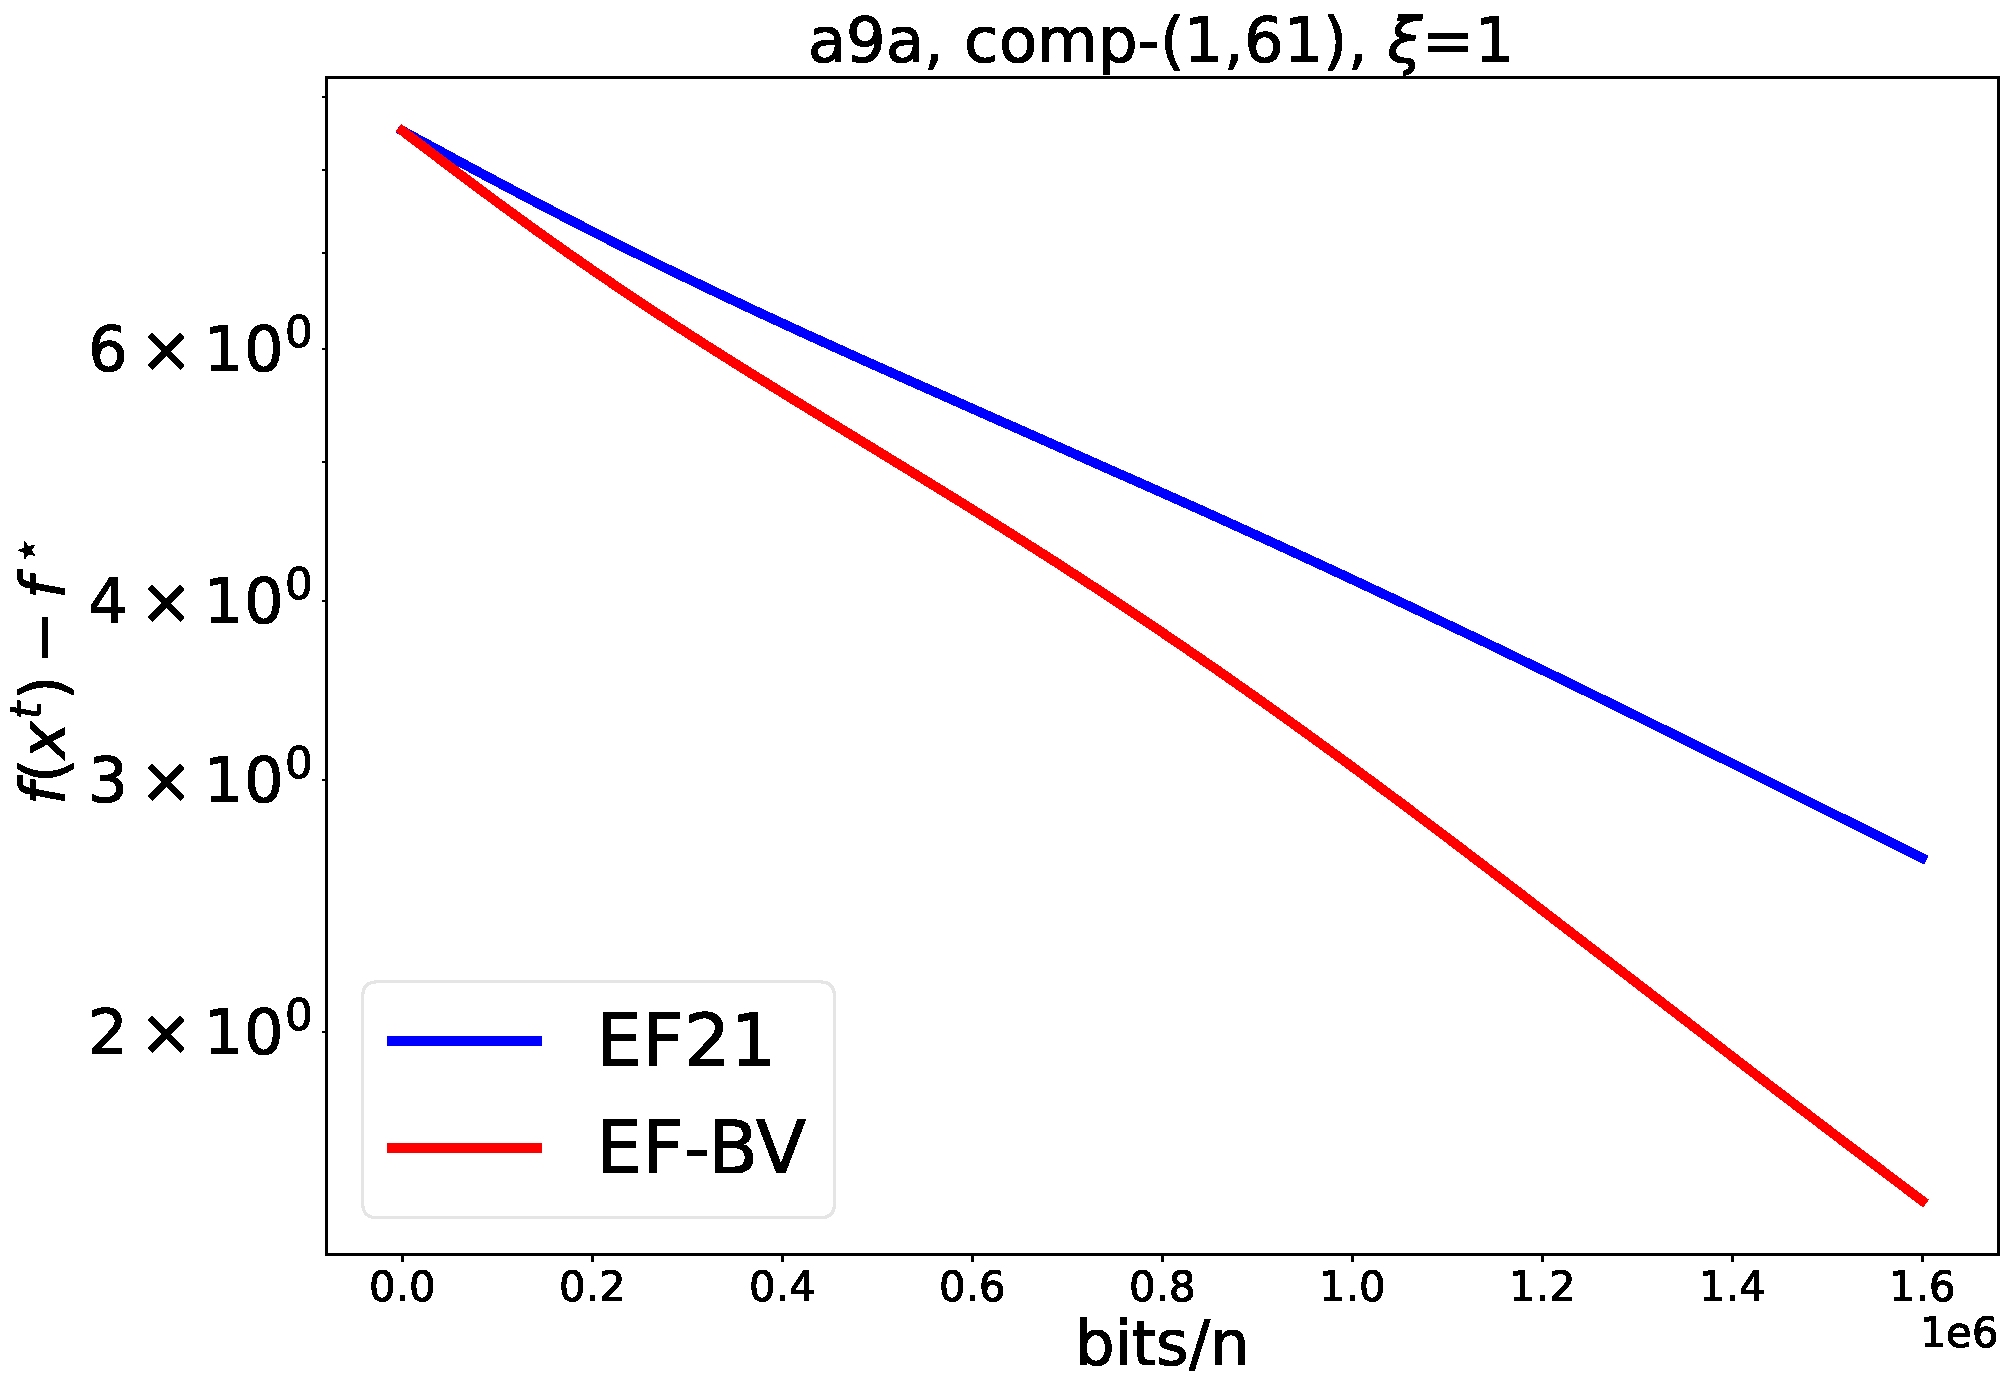
\includegraphics[width=\textwidth]{img/a9a/CompK_61_1_a9a_8124workers_3000K_32561_a9a_61_1_1_1_logreg_diff_nonconv.pdf}
   \end{subfigure}
   \hfill
   \begin{subfigure}[b]{0.32\textwidth}
      \centering
      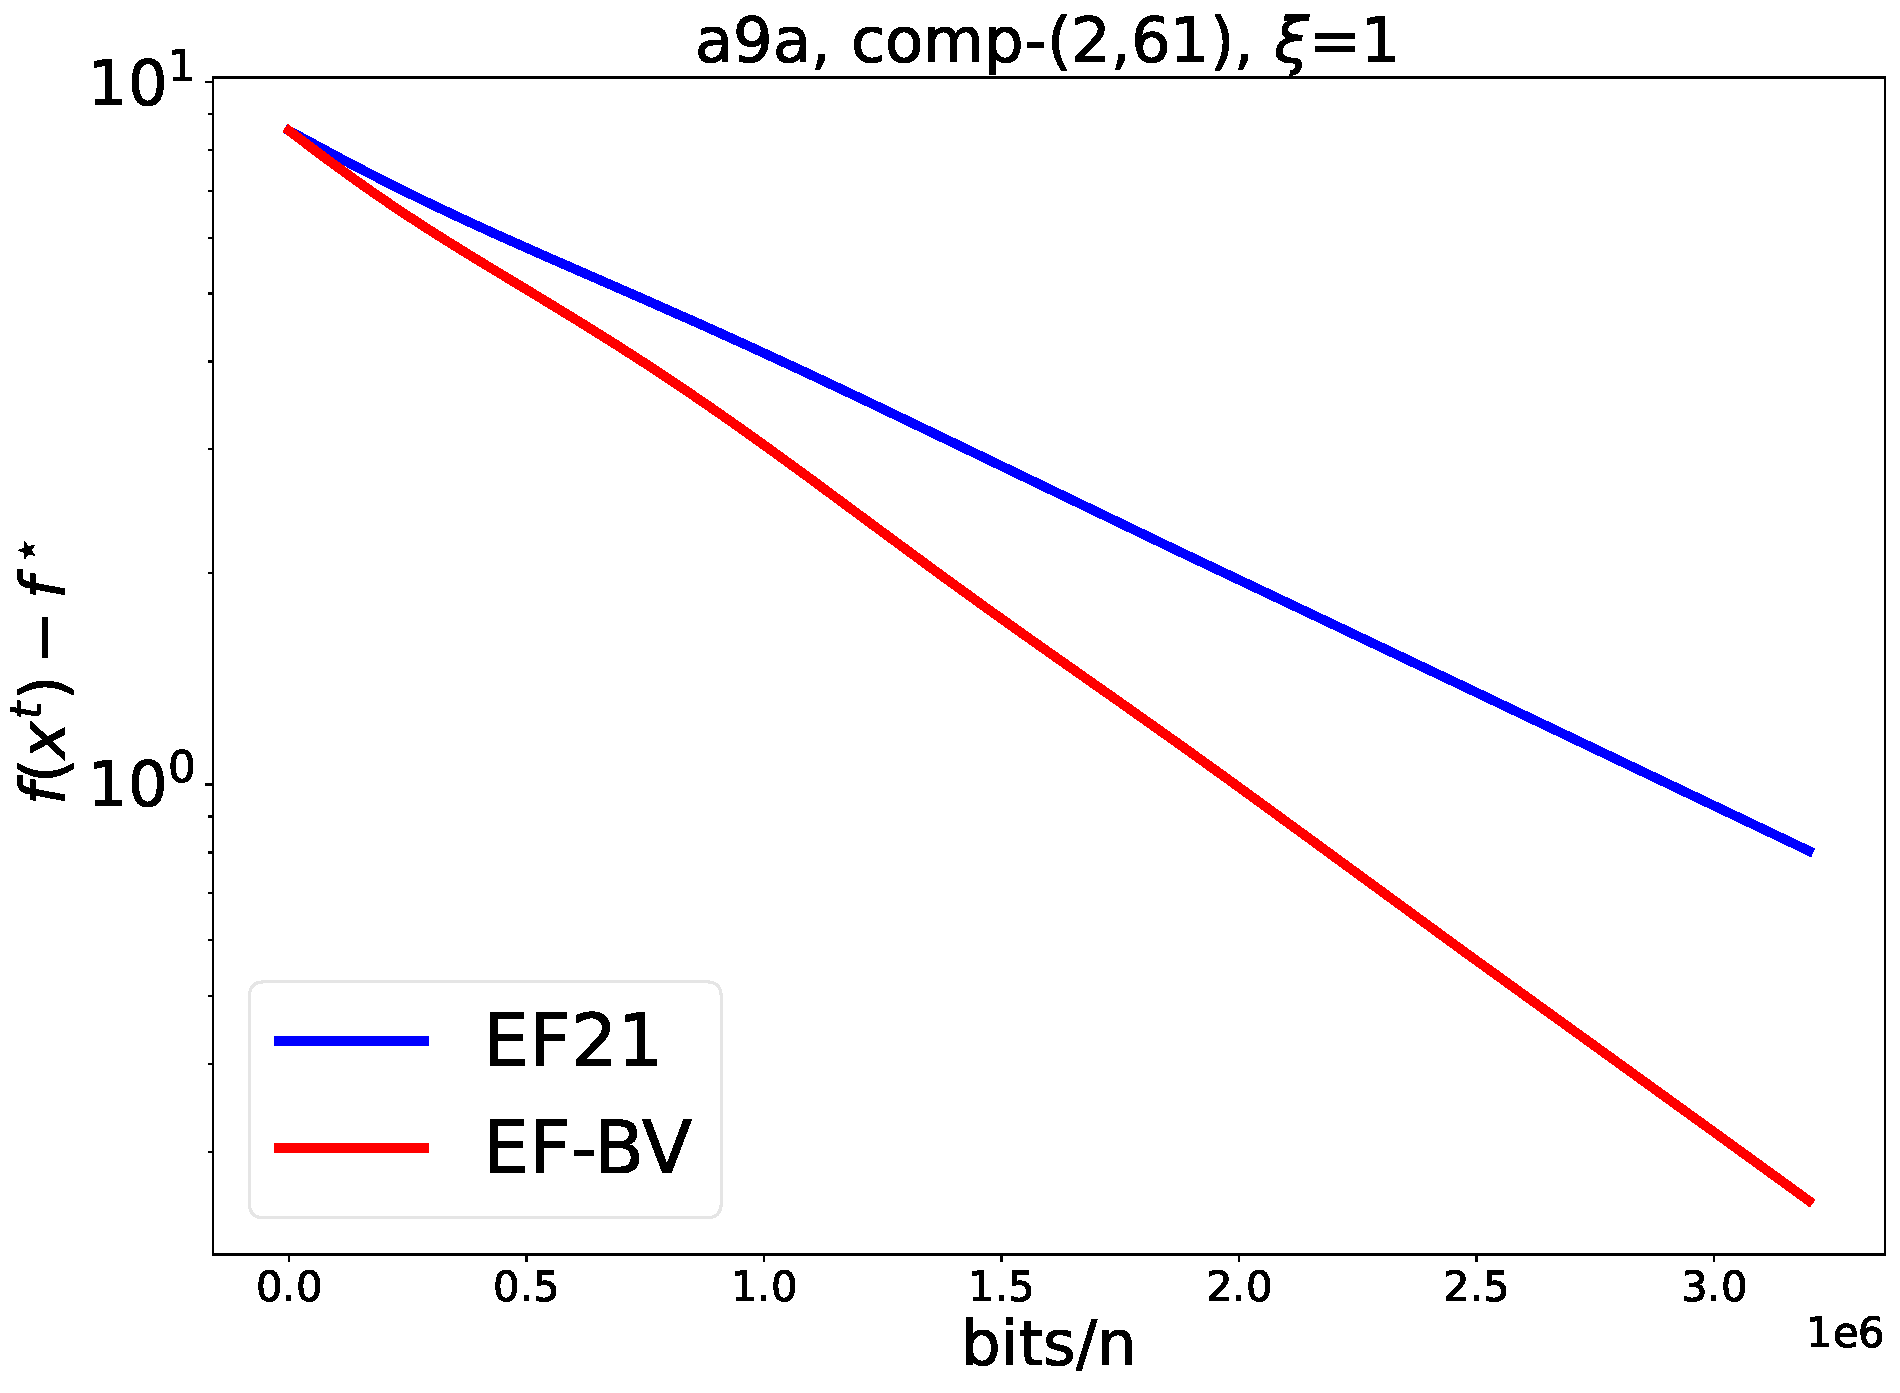
\includegraphics[width=\textwidth]{img/a9a/CompK_61_2_a9a_8124workers_3000K_32561_a9a_61_2_1_1_logreg_diff_nonconv.pdf}
   \end{subfigure}
   \hfill
   \begin{subfigure}[b]{0.32\textwidth}
      \centering
      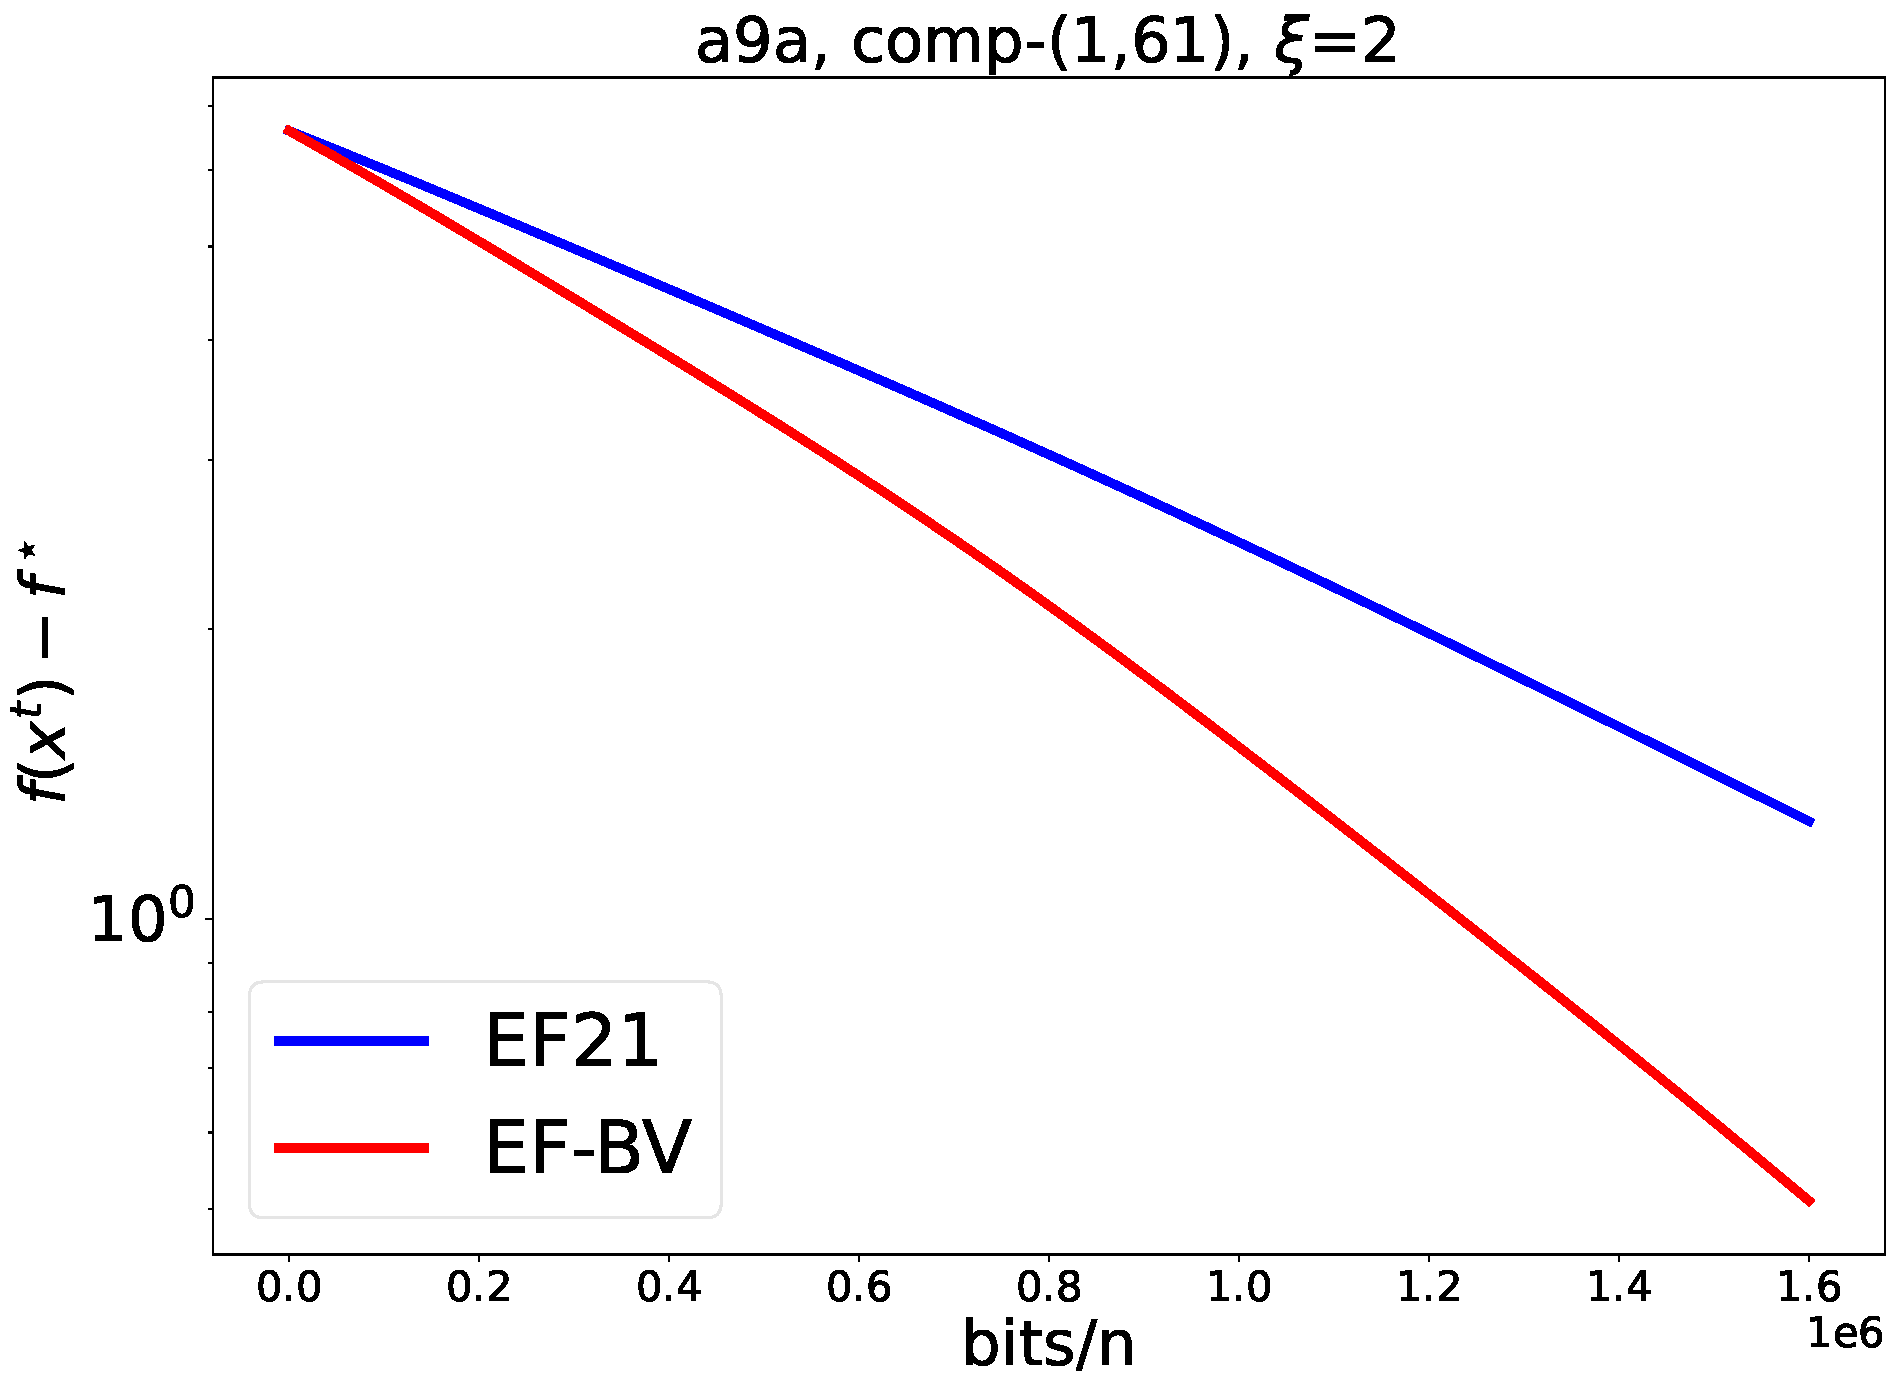
\includegraphics[width=\textwidth]{img/a9a/CompK_61_1_a9a_8124workers_3000K_32561_a9a_61_1_1_2_logreg_diff_nonconv.pdf}
   \end{subfigure}
   \hfill
   \begin{subfigure}[b]{0.32\textwidth}
      \centering
      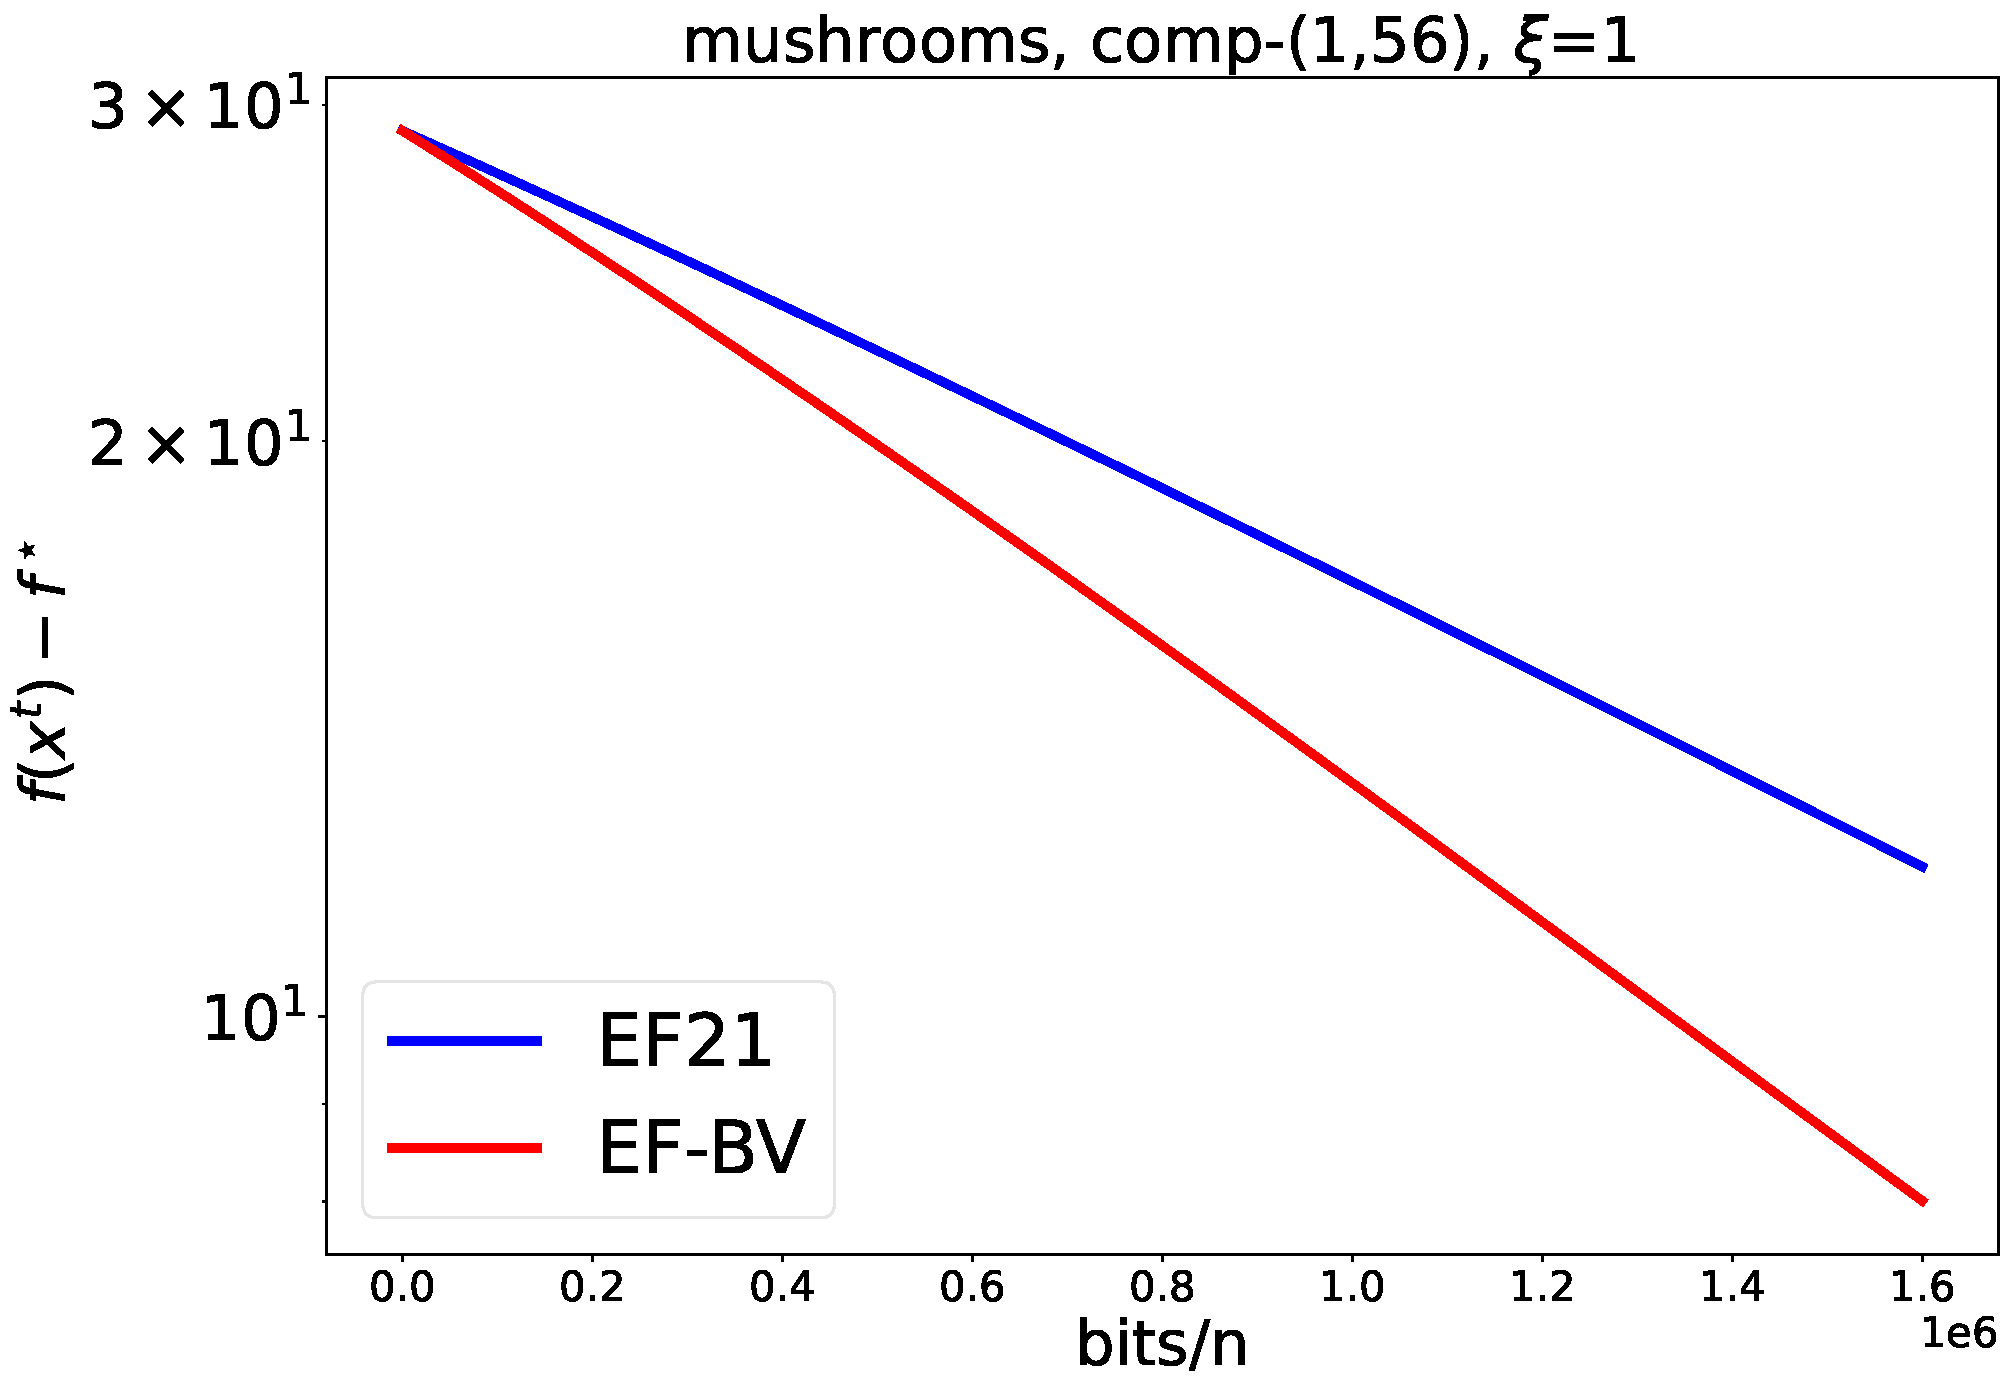
\includegraphics[width=\textwidth]{img/mushrooms/CompK_56_1_mushrooms_8124workers_3000K_8124_mushrooms_56_1_1_1_logreg_diff_nonconv.pdf}
   \end{subfigure}
   \hfill
   \begin{subfigure}[b]{0.32\textwidth}
      \centering
      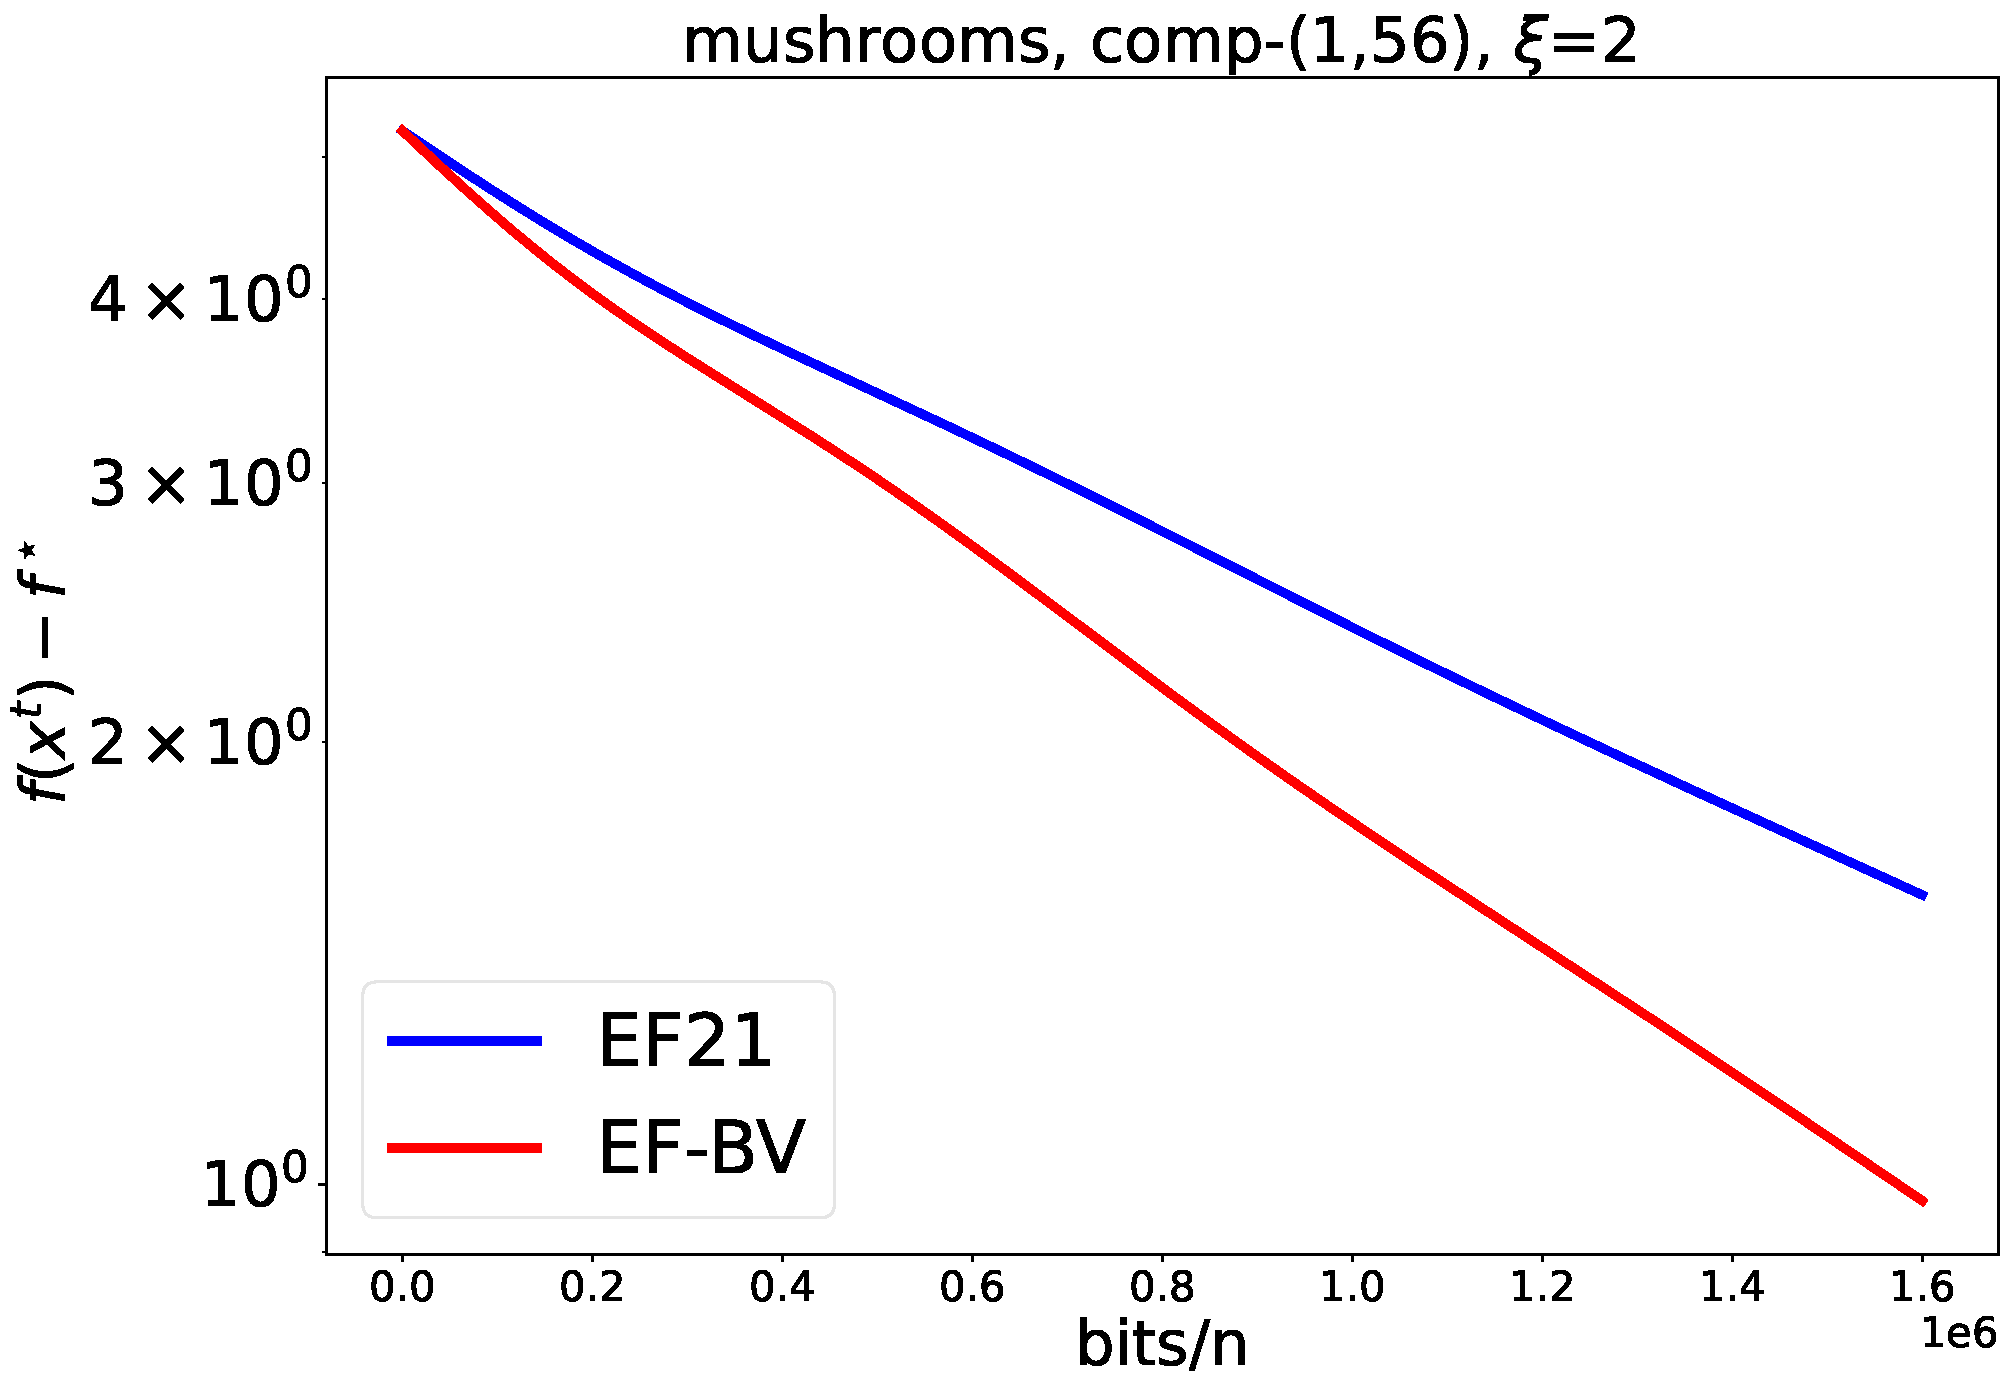
\includegraphics[width=\textwidth]{img/mushrooms/CompK_56_1_mushrooms_8124workers_3000K_8124_mushrooms_56_1_1_2_logreg_diff_nonconv.pdf}
   \end{subfigure}
   \hfill
   \begin{subfigure}[b]{0.32\textwidth}
      \centering
      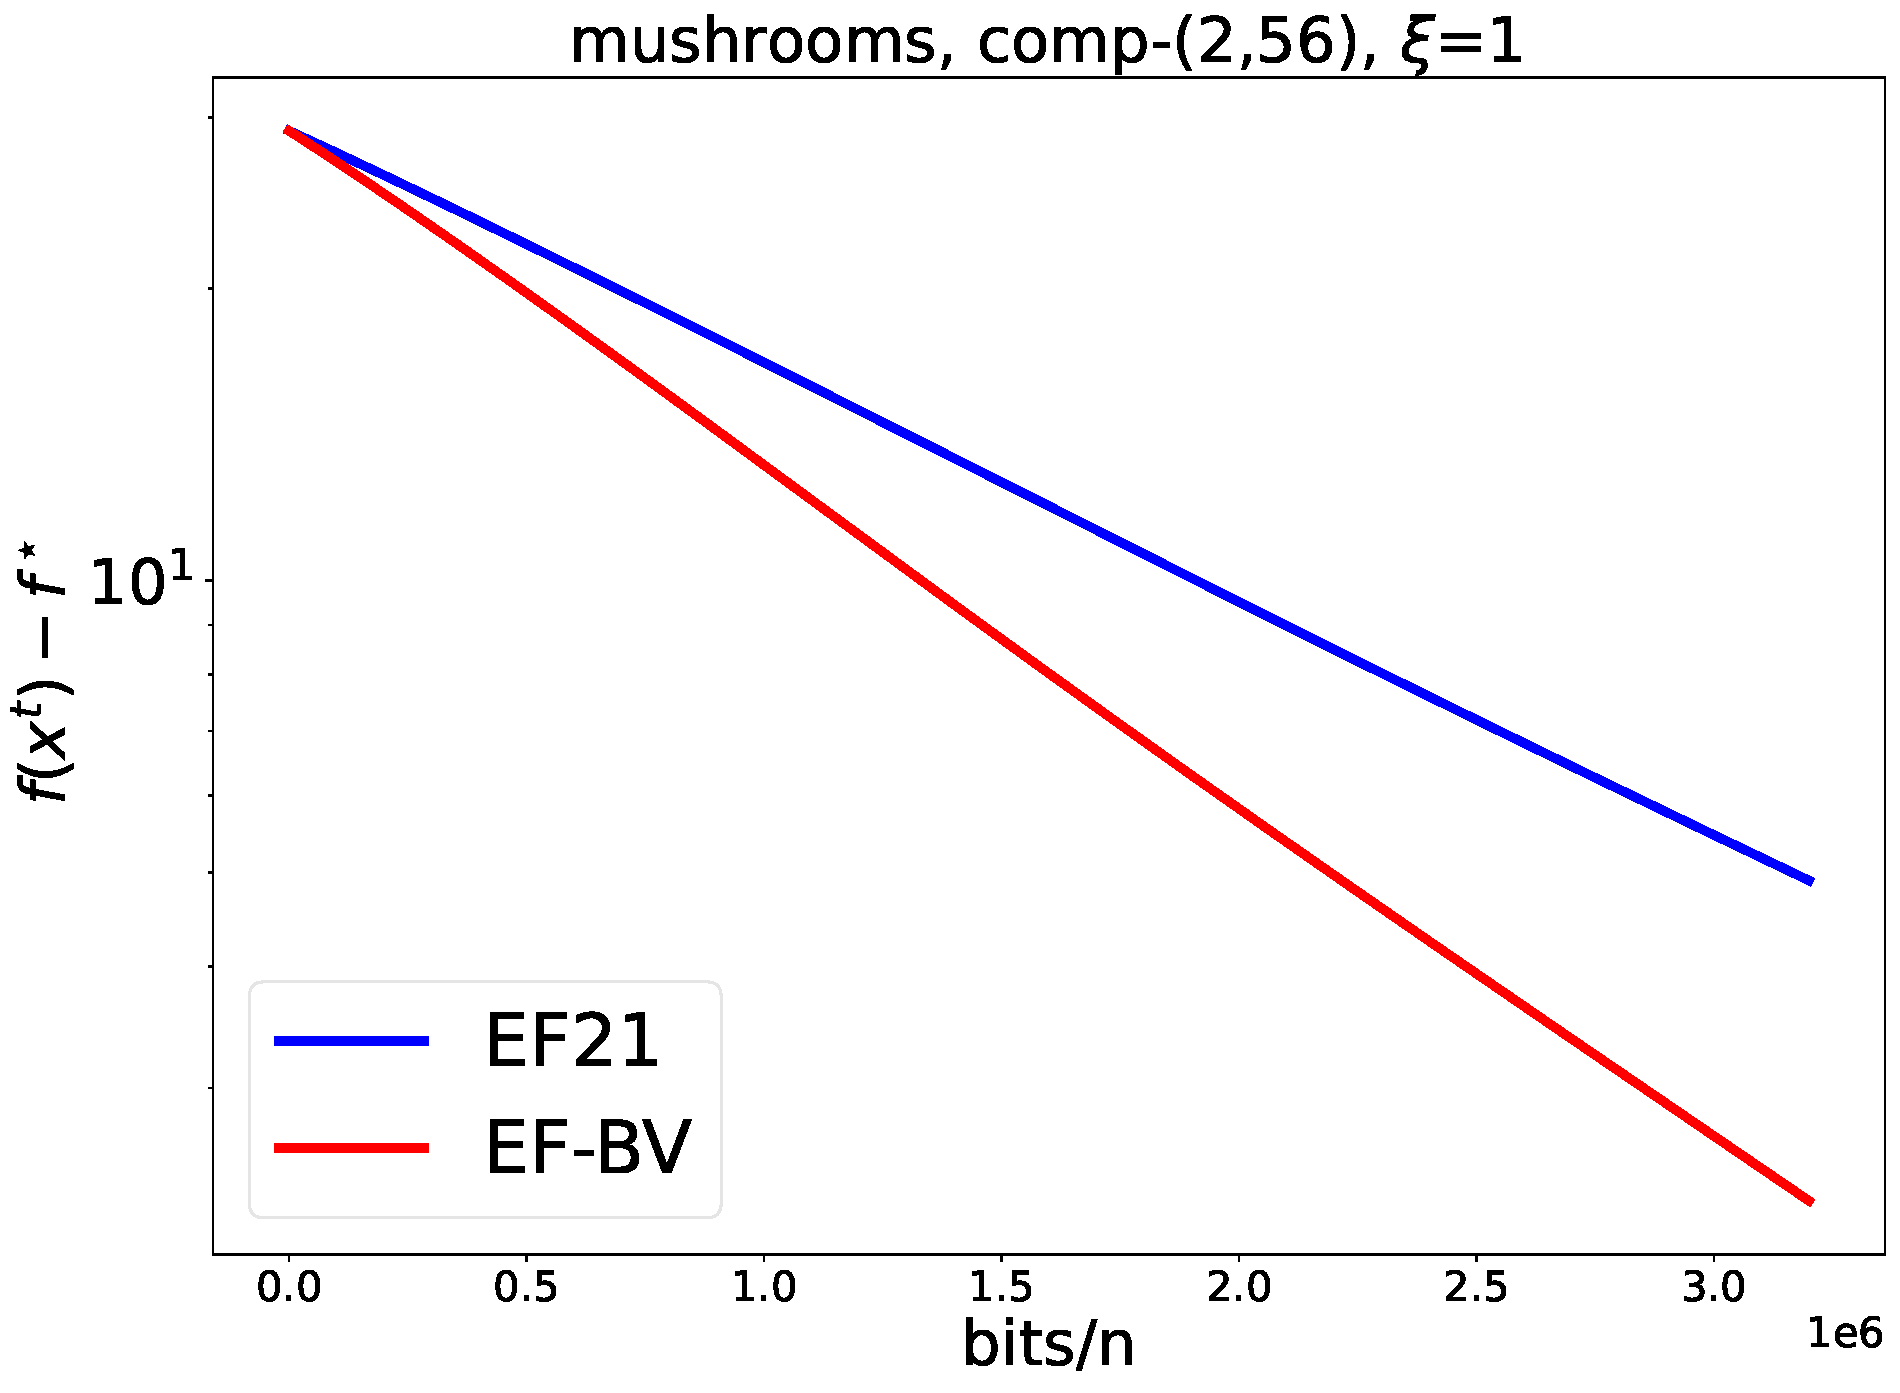
\includegraphics[width=\textwidth]{img/mushrooms/CompK_56_2_mushrooms_8124workers_3000K_8124_mushrooms_56_2_1_1_logreg_diff_nonconv.pdf}
   \end{subfigure}
   \hfill
   \begin{subfigure}[b]{0.32\textwidth}
      \centering
      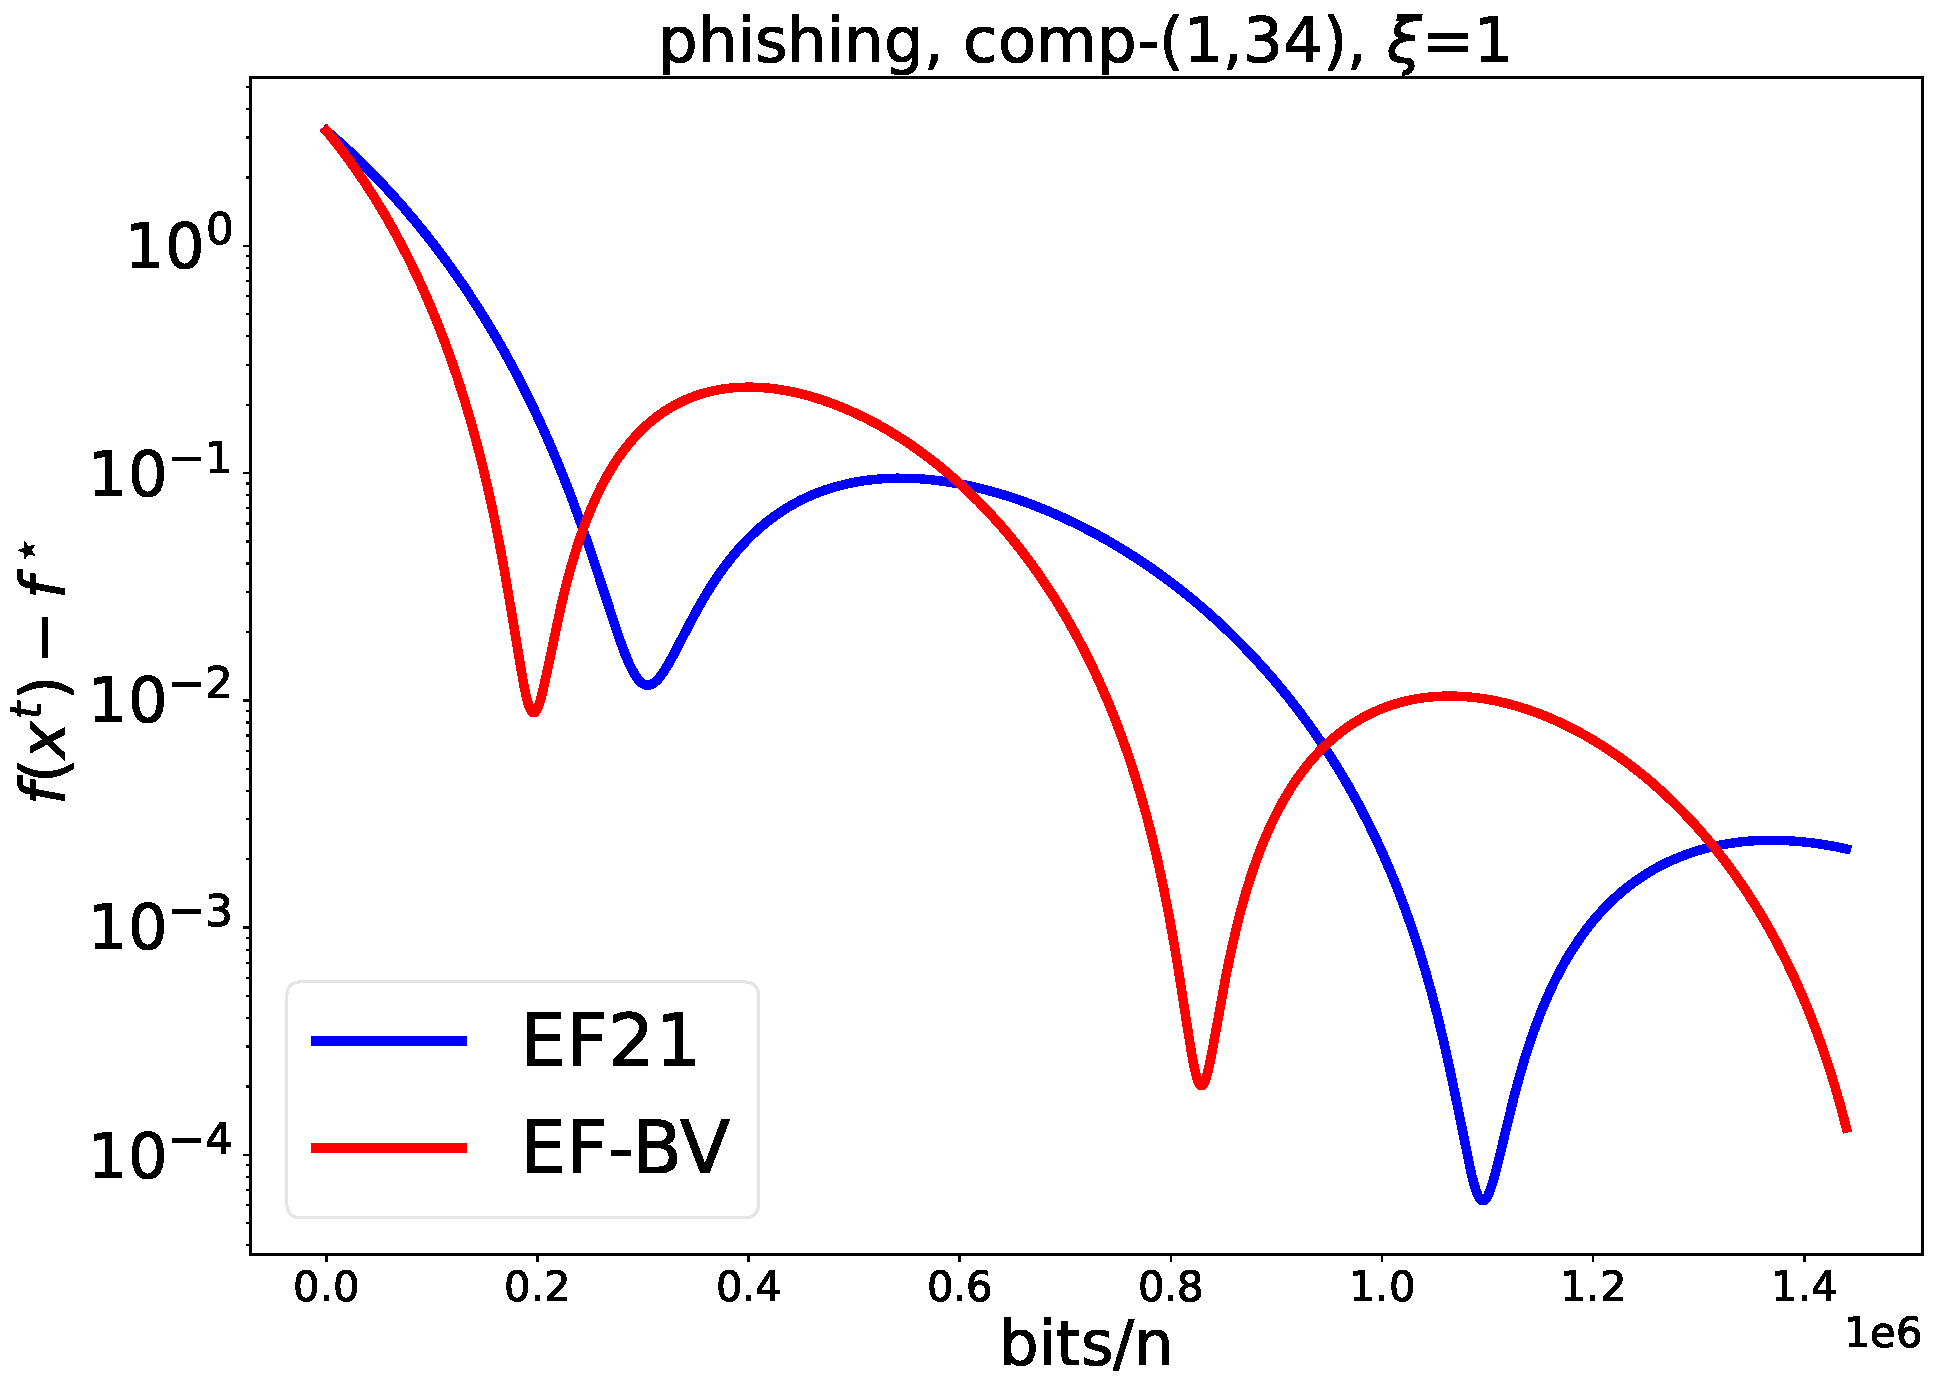
\includegraphics[width=\textwidth]{img/phishing/CompK_34_1_phishing_8124workers_3000K_11055_phishing_34_1_1_1_logreg_diff_nonconv.pdf}
   \end{subfigure}
   \hfill
   \begin{subfigure}[b]{0.32\textwidth}
      \centering
      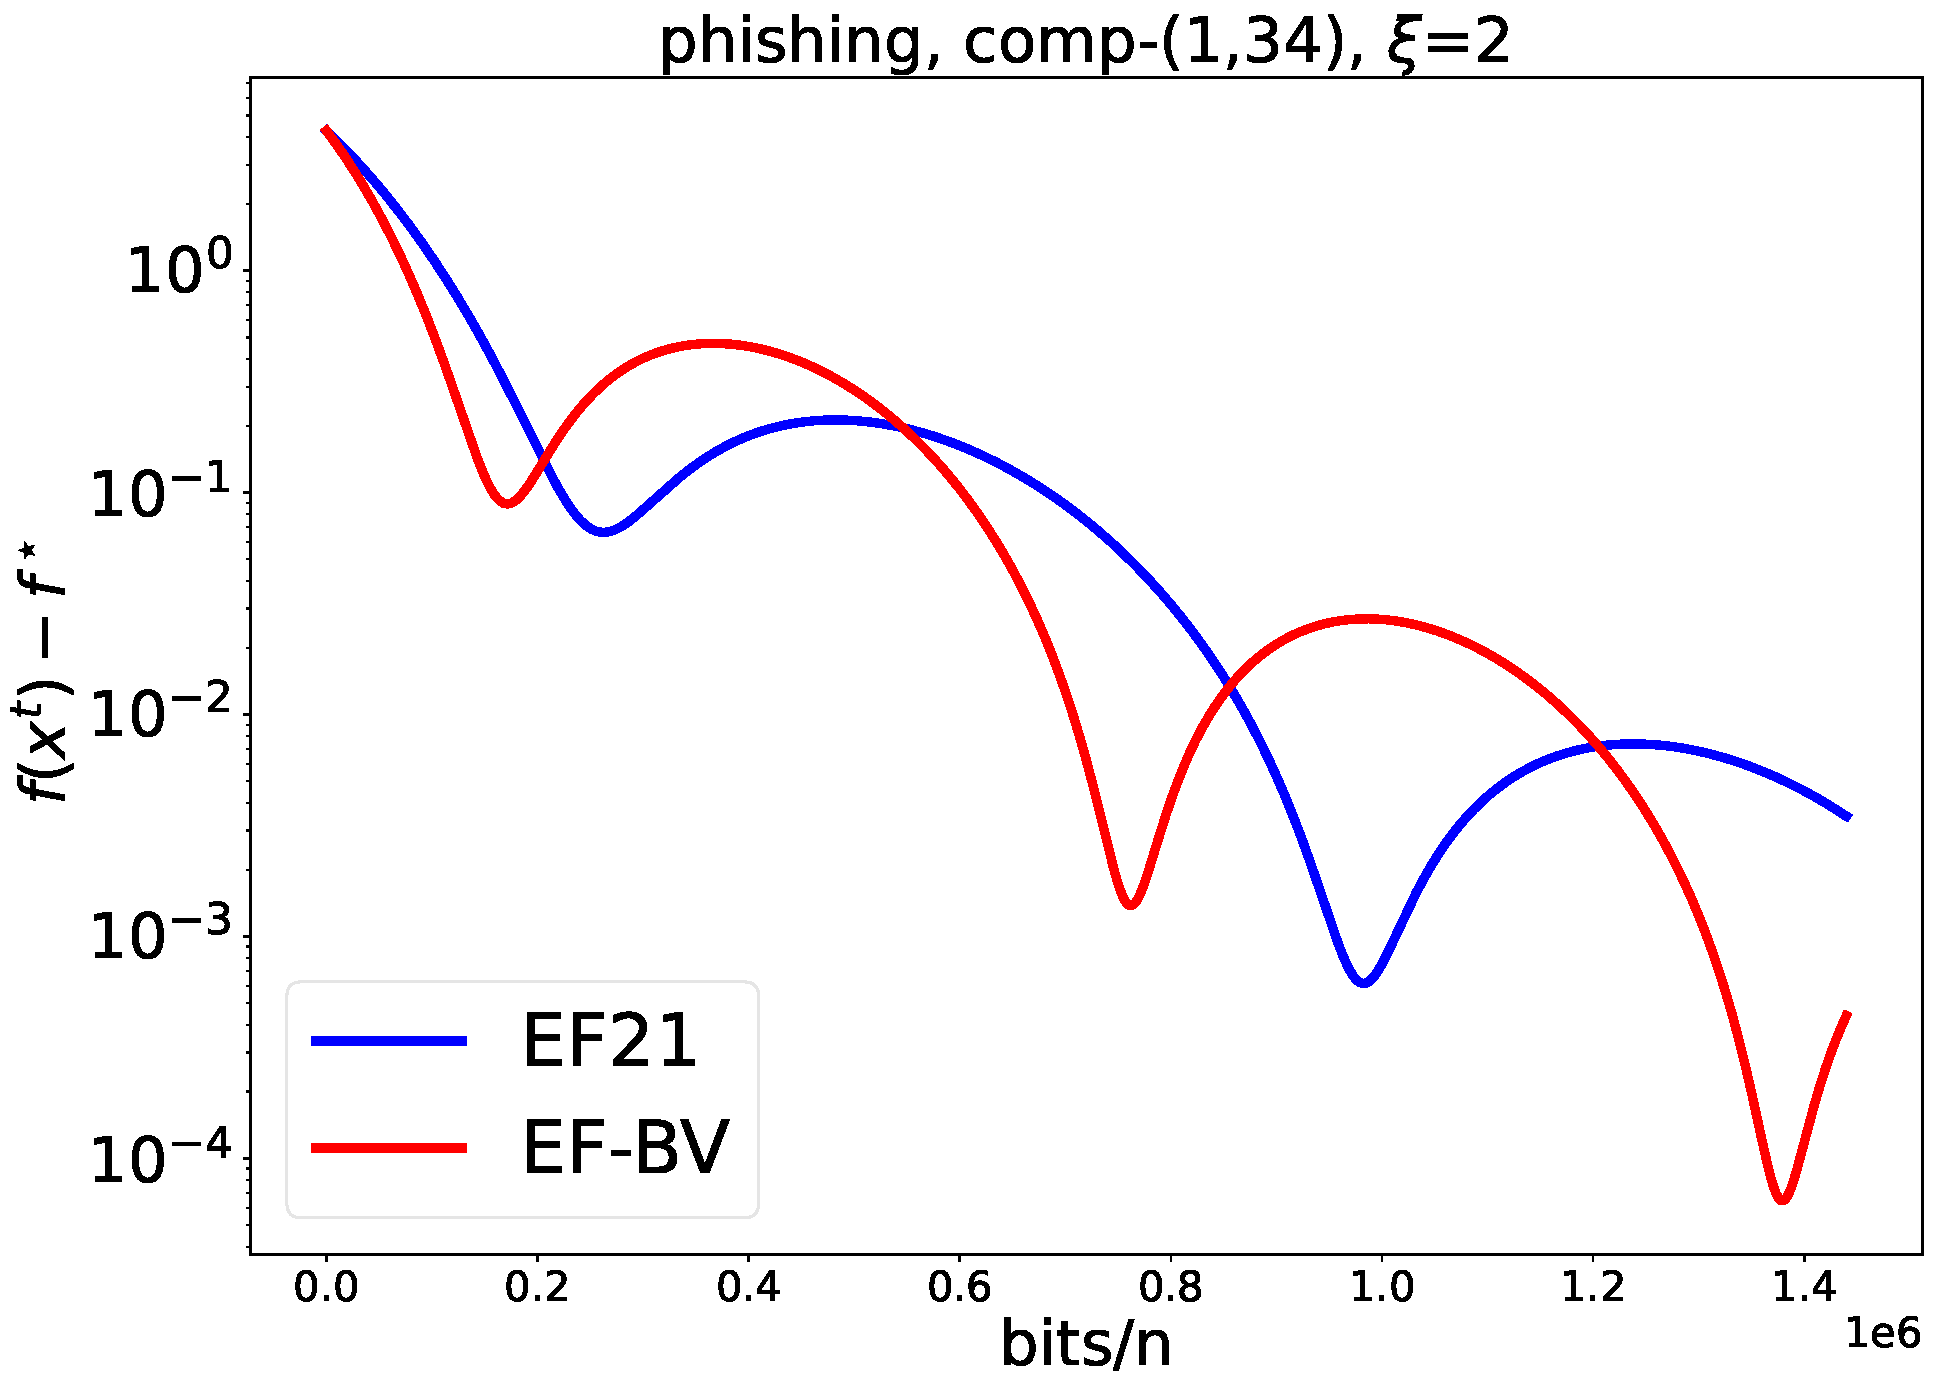
\includegraphics[width=\textwidth]{img/phishing/CompK_34_1_phishing_8124workers_3000K_11055_phishing_34_1_1_2_logreg_diff_nonconv.pdf}
   \end{subfigure}
   \hfill
   \begin{subfigure}[b]{0.32\textwidth}
      \centering
      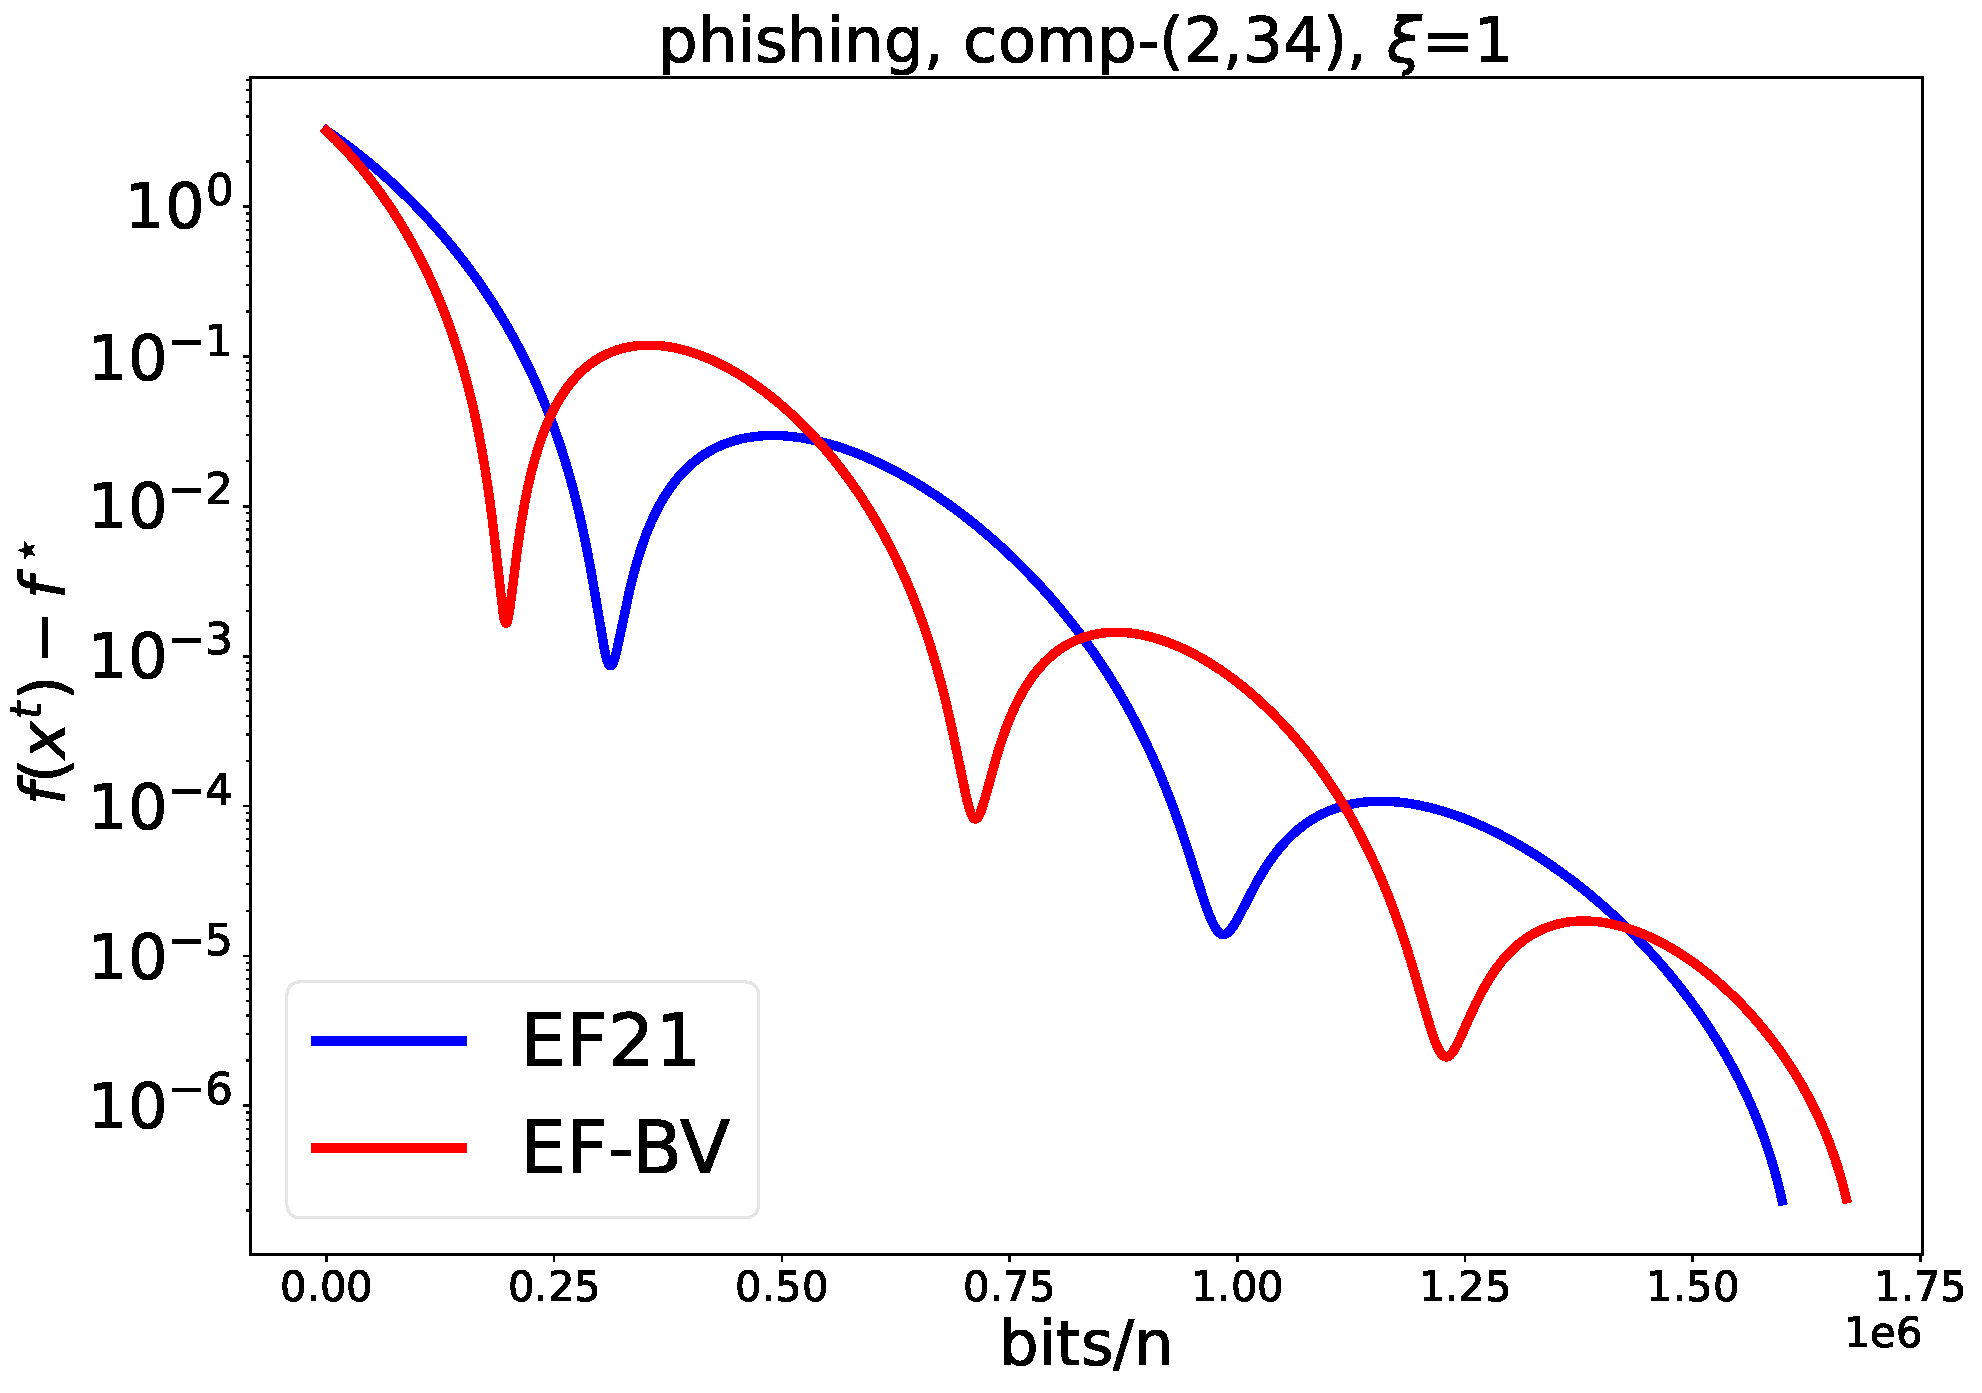
\includegraphics[width=\textwidth]{img/phishing/CompK_34_2_phishing_8124workers_3000K_11055_phishing_34_2_1_1_logreg_diff_nonconv.pdf}
   \end{subfigure}
   % \hfill
   % \begin{subfigure}[b]{0.32\textwidth}
   %    \centering
   %    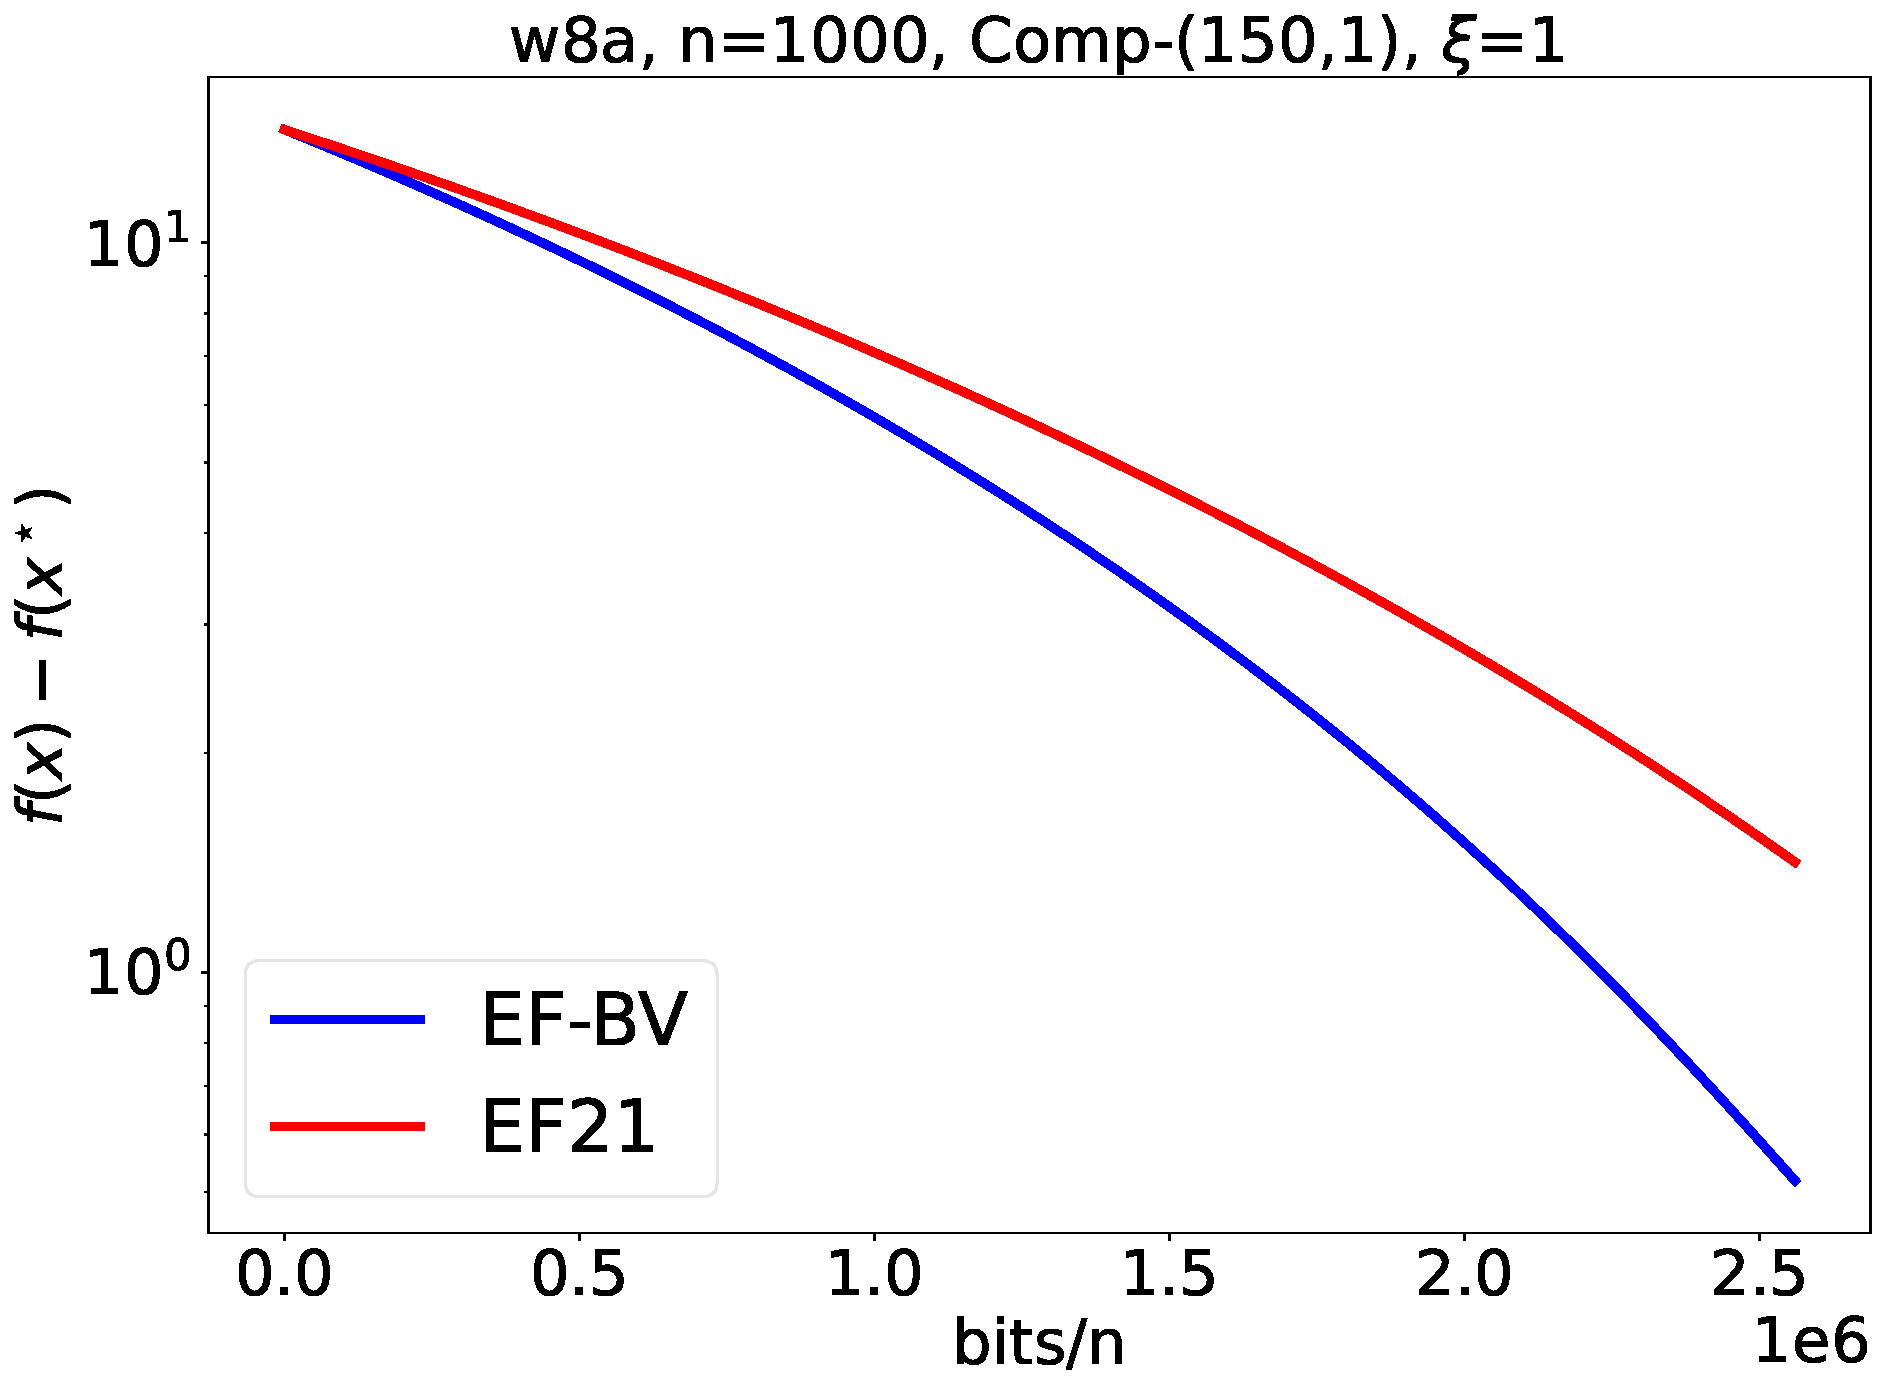
\includegraphics[width=\textwidth]{img/w8a/CompK_150_1_w8a_20workers_3000K_1000_w8a_1_1_logreg_diff.pdf}
   %    % \caption{no partial participation}
   %    \label{010}
   % \end{subfigure}
   % \hfill
   % \begin{subfigure}[b]{0.32\textwidth}
   %    \centering
   %    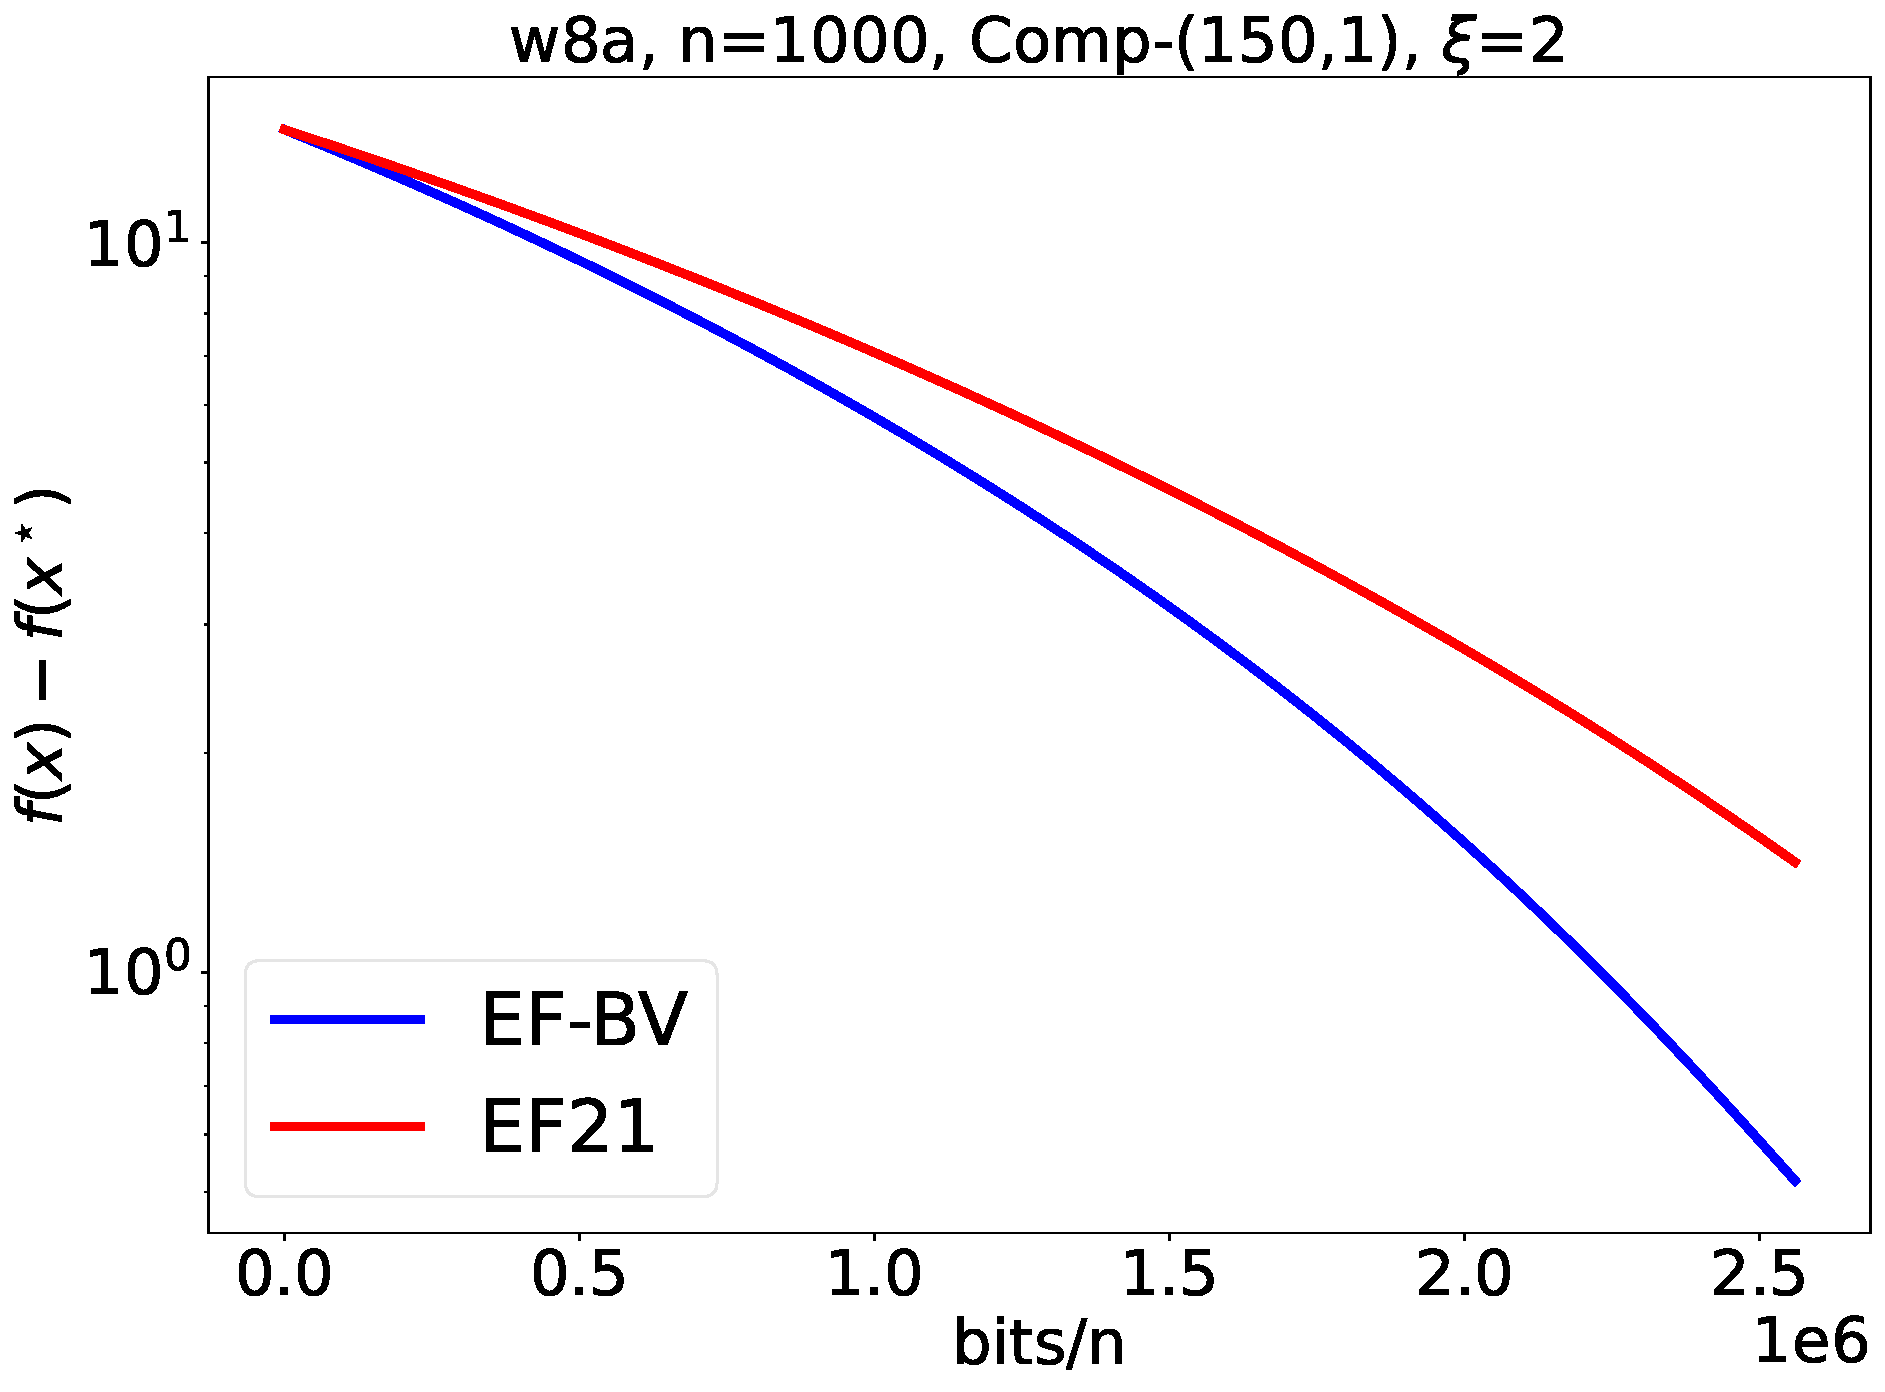
\includegraphics[width=\textwidth]{img/w8a/CompK_150_1_w8a_20workers_3000K_1000_w8a_1_2_logreg_diff.pdf}
   %    % \caption{no partial participation}
   %    \label{011}
   % \end{subfigure}
   % \hfill
   % \begin{subfigure}[b]{0.32\textwidth}
   %    \centering
   %    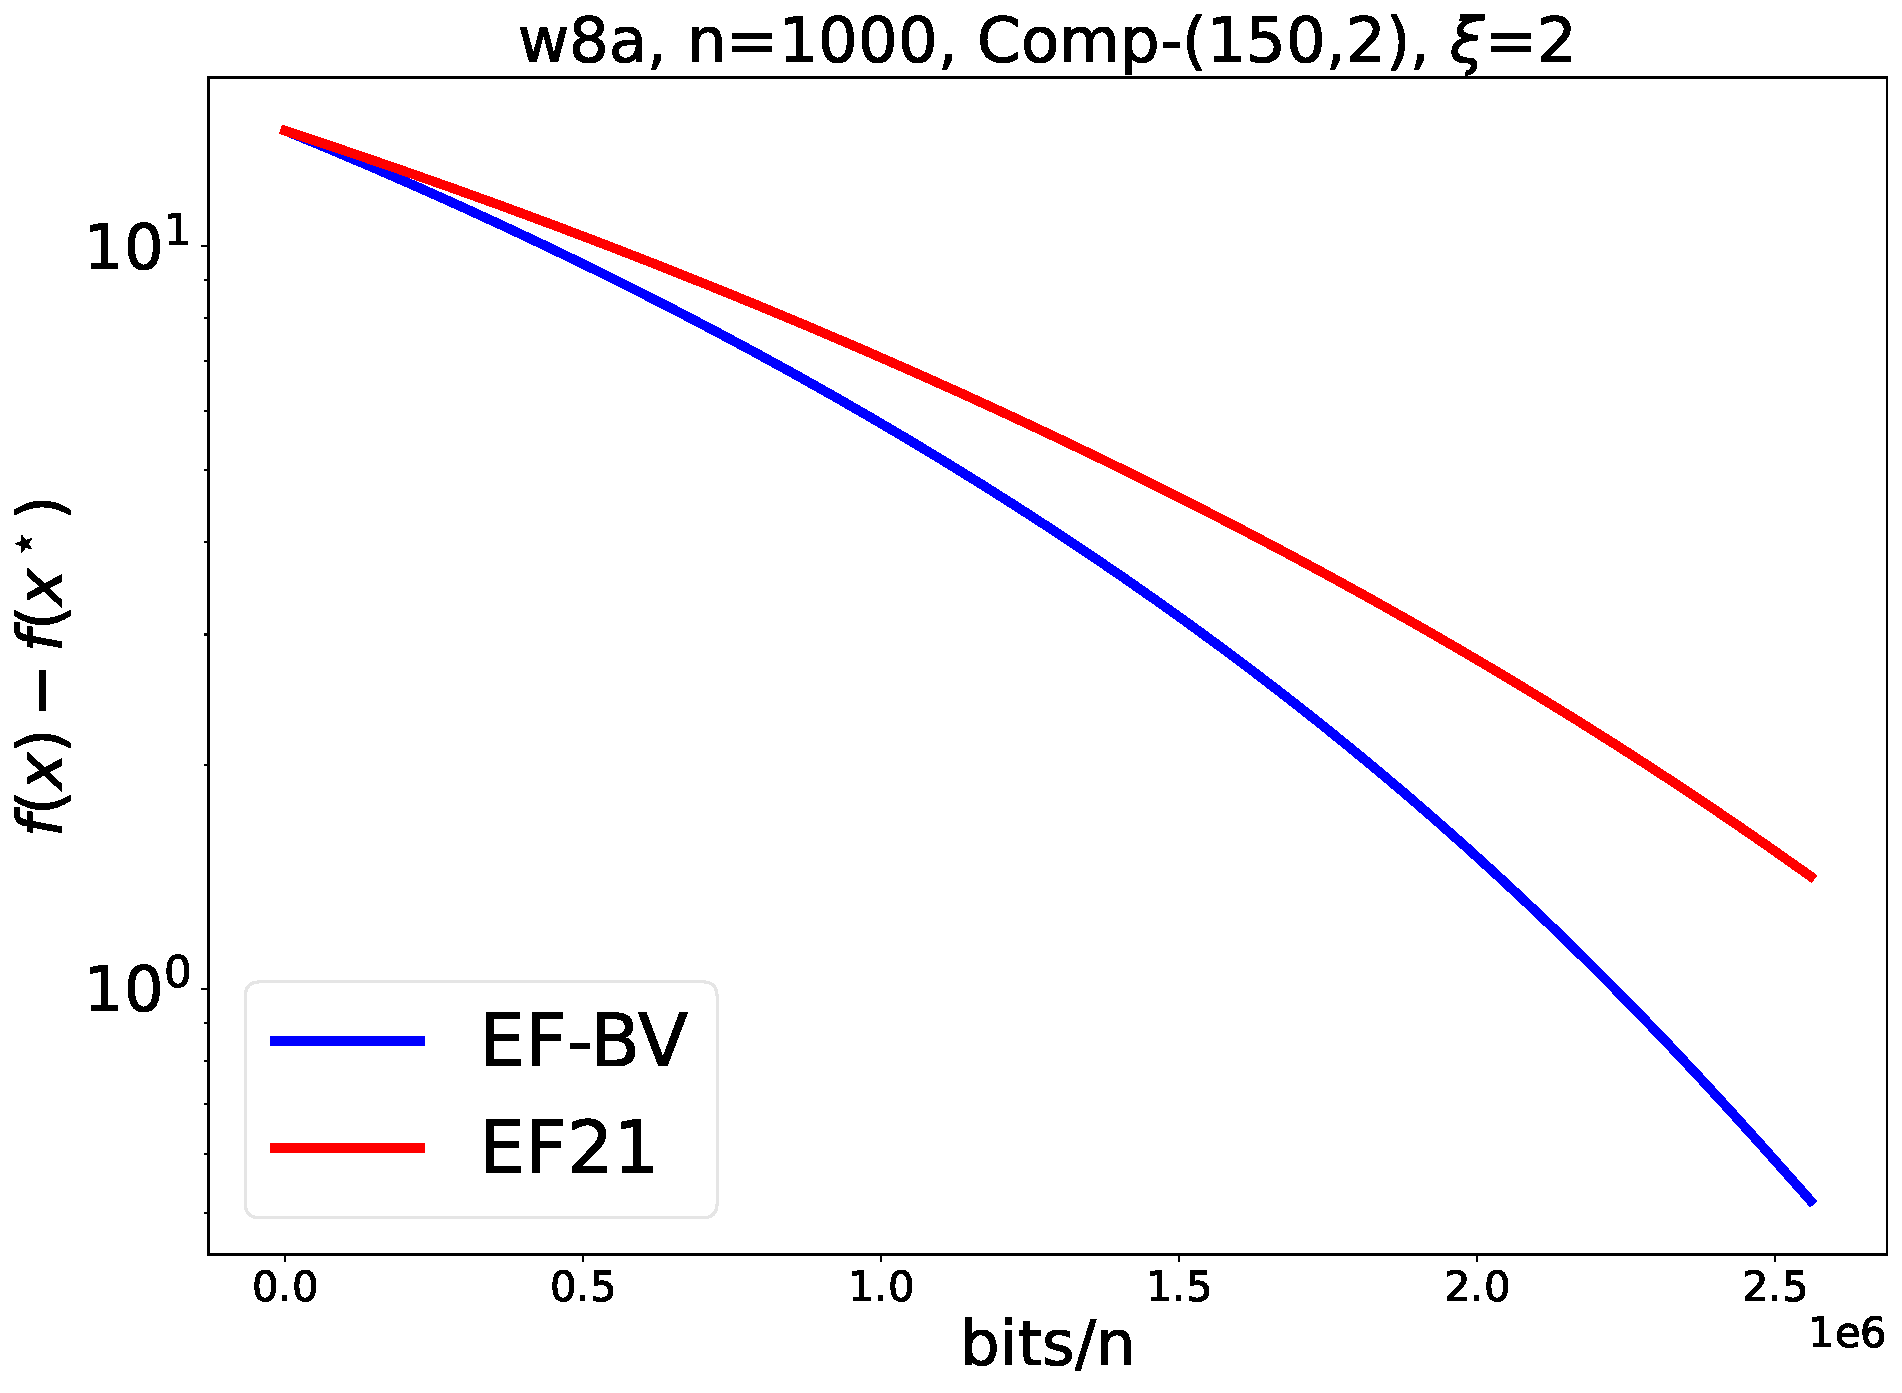
\includegraphics[width=\textwidth]{img/w8a/CompK_150_2_w8a_20workers_3000K_1000_w8a_1_2_logreg_diff.pdf}
   %    % \caption{$\tau=1, lrr=0.1, pr=0.2$}
   %    \label{012}
   % \end{subfigure}
      \caption{Comparison between \algname{EF21} and \algname{EF-BV} in the non-convex setting. We see \algname{EF-BV} outperforms \algname{EF21} on all datasets.}
      \label{13}
\end{figure}

\subsection{Other Options}
\subsubsection{Least squares}
Here we consider the function that satisfies the PL condition. We use the standard least squares objective function, 

\begin{equation}
   f(x)=\frac{1}{n} \sum_{i=1}^{n}\left(a_{i}^{\top} x-b_{i}\right)^{2},
\end{equation}

where $a_{i} \in \mathbb{R}^{d}, y_{i} \in\{-1,1\}$ are the training data.

We can extend to least squares if we want later. 

\subsubsection{Deep neural networks}
We also consider the deep neural networks experiments. To make fair comparison, we choose CIFAR-10 as our target dataset, which contains 50, 000 images for training and 10,000 images for testing. We randomly split the whole training set and testing set into n=5 equal part. Similar to \algname{EF21}~\cite{ric21}, we consider models including ResNet18 and VGG11. 

From \algname{EF21}~\cite{ric21} Fig.13, 14 and 15, we found \algname{EF21} use tuned stepsizes. However, the advantage of \algname{EF-BV} is that we have much larger stepsize under centain conditions. So here I pend the comparison with \algname{EF21} on deep neural networks. 
% \subsection{Algorithm Description}
% \begin{algorithm}[!htbp]
% \caption{EF-BV for single node}\label{alg:efbv_1}
% \begin{algorithmic}
% \Require stepsize $\gamma>0$, initial iterate $x^{0} \in \R^{d}$; initial shift {$h^0$} $\in \R^{d}$, \sybg{$\lambda\in (0, 1]$}, \sybr{$\nu \in (0,1]$} 
% \For{t = 0, 1, 2, $\cdots$}
%     \State Compute the gradient: $\nabla f\left(x^{t}\right)$
%     \State Compress shifted gradient: {$m^{t}$} $=\mathcal{C}(\nabla f\left(x^{t}\right)-$ {$h^{t})$}
%     \State Compute gradient estimator: $g^{t}=$ {$h^{t}$} + \sybr{$\nu$}{$m^{t}$}
%     \State Take proximal SGD step: $x^{t+1}=\operatorname{prox}_{\gamma R}\left(x^{t}-\gamma g^{t}\right)$
%     \State Update the shift: {$h^{t+1}$}={$h^{t}$} $+$ \sybg{$\lambda$} {$m^{t}$}
% \EndFor 
% \end{algorithmic}
% \end{algorithm}

\bibliography{mybib}
\bibliographystyle{iclr2021_conference}

\newpage
\appendix


\section{Appendix}
\subsection{Missing proofs}
\subsubsection{Missing proof of Theorem~\ref{thm:main}}
$g_i^t = h_i^t + \nu \C(\nabla f_i (x^t) - h_i^t); \quad h_i^{t+1} = h_i^t + \lambda \C(\nabla f_i (x^t) - h_i^t)$

\begin{proof}
   We first bound $\E\left[\|g_i^{t+1} - \nabla f_i(x^{t})\|^2\right]$. 

   Given any compressor $\mathcal{C}$, we can do a {\it bias-variance decomposition} of the compression error (see Eqn.~\ref{eqbiva}). 
   % That means, for every $x\in\mathbb{R}^d$,
   % \begin{equation}
   %  \mathbb{E}\big[\|\mathcal{C}(x)-x\|^2\big] = {\underbrace{\big\| \mathbb{E}[\mathcal{C}(x)]-x\big\|}_{\text{bias}}}^2 + \underbrace{\mathbb{E}\Big[\big\|\mathcal{C}(x)-\mathbb{E}[\mathcal{C}(x)]\big\|^2\Big]}_{\text{variance}}.\label{eqbiva}
   %  \end{equation}
   For every $t\geq 0$, define $W^t = \{x^t, h^t, (h_i^t)_{i=1}^n\}$,
   \begin{equation}\label{eq0001}
   \begin{aligned}
      \Exp{\sqnorm{g^{t+1}-\nabla f(x^t)} | W^t} &=\Exp{\sqnorm{\frac{1}{n}\sum_{i=1}^n \Big(h_i^{t}-\nabla f_i(x^t) +\nu \mathcal{C}_i^t\big(\nabla f_i(x^t)-h_i^t\big) \Big) } | W^t}\\
      &\stackrel{(\ref{eqbiva})}{=}\sqnorm{\frac{1}{n}\sum_{i=1}^n \Big(h_i^{t}-\nabla f_i(x^t) +\nu \Exp{\mathcal{C}_i^t\big(\nabla f_i(x^t)-h_i^t\big)} \Big) | W^t} \\
      &\quad+\nu^2\Exp{\sqnorm{\frac{1}{n}\sum_{i=1}^n \Big( \mathcal{C}_i^t\big(\nabla f_i(x^t)-h_i^t\big)-\Exp{ \mathcal{C}_i^t\big(\nabla f_i(x^t)-h_i^t\big) } \Big) } | W^t}\\
      &\leq \sqnorm{\frac{1}{n}\sum_{i=1}^n \Big(h_i^{t}-\nabla f_i(x^t) +\nu \Exp{\mathcal{C}_i^t\big(\nabla f_i(x^t)-h_i^t\big)} \Big) | W^t}\\
      &\quad+\nu^2 \frac{\oma}{n}\sum_{i=1}^n \sqnorm{\nabla f_i(x^t)-h_i^t },
   \end{aligned}      
   \end{equation}
   where the last inequality follows from Eqn.~7 in \cite{condat2022ef}. In addition, using Jensen's inequality and the definition of general compressor (Eqn.~\ref{def:compressors}), 
 
   % \kai{TODO: check where W^t can be omit from EF21-Lemma2}
   \begin{equation}\label{eq0002}
   \begin{aligned}
      &\left\|\frac{1}{n}\sum_{i=1}^n \Big(h_i^{t}-\nabla f_i(x^t) +\nu \Exp{\mathcal{C}_i^t\big(\nabla f_i(x^t)-h_i^t\big)} \Big) | W^t\right\|\\
      &\quad \leq \left\|\frac{1}{n}\sum_{i=1}^n \Big(\nu\big(h_i^{t}-\nabla f_i(x^t)\big) +\nu \Exp{\mathcal{C}_i^t\big(\nabla f_i(x^t)-h_i^t\big)} \Big) | W^t\right\| + (1-\nu)\left\|\frac{1}{n}\sum_{i=1}^n \big(h_i^{t}-\nabla f_i(x^t)\big)\right\|\\
      &\quad \leq \frac{\nu}{n}\sum_{i=1}^n\left\|h_i^{t}-\nabla f_i(x^t)+ \Exp{\mathcal{C}_i^t\big(\nabla f_i(x^t)-h_i^t\big)} | W^t\right\| + \frac{1-\nu}{n}\sum_{i=1}^n \left\|h_i^{t}-\nabla f_i(x^t)\right\|\\
      &\quad \leq  \frac{\nu\eta}{n}\sum_{i=1}^n \left\|\nabla f_i(x^t)-h_i^{t}\right\|+ \frac{1-\nu}{n}\sum_{i=1}^n \left\|\nabla f_i(x^t)-h_i^{t}\right\|\\
      & \quad = \frac{1-\nu+\nu\eta}{n}\sum_{i=1}^n \left\|\nabla f_i(x^t)-h_i^{t}\right\|.
   \end{aligned}
   \end{equation}
   Therefore, 
   \begin{align*}
   \sqnorm{\frac{1}{n}\sum_{i=1}^n \Big(h_i^{t}-\nabla f_i(x^t) +\nu \Exp{\mathcal{C}_i^t\big(\nabla f_i(x^t)-h_i^t\big)} \Big) | W^t} \leq \frac{(1-\nu+\nu\eta)^2}{n}\sum_{i=1}^n \sqnorm{\nabla f_i(x^t)-h_i^{t}}.
   \end{align*}

   Putting Eq.~\ref{eq0002} into Eq.~\ref{eq0001}, we have 
   
   \begin{align*}
   \Exp{\sqnorm{g^{t+1}-\nabla f(x^t)}| W^t} &\leq 
   \left((1-\nu+\nu\eta)^2+\nu^2\oma\right)\frac{1}{n}\sum_{i=1}^n \sqnorm{\nabla f_i(x^t)-h_i^{t}}.
   \end{align*}

   Using the Tower property and we obtain the unconditioned term,
   \begin{align*}
      \Exp{\sqnorm{g^{t+1}-\nabla f(x^t)}} &\leq 
      \left((1-\nu+\nu\eta)^2+\nu^2\oma\right)\frac{1}{n}\sum_{i=1}^n \Exp{\sqnorm{\nabla f_i(x^t)-h_i^{t}}}.
      \end{align*}
    
   Since we have the property \citep[Lemma 4]{ric21}, for every $t\geq 0$,
   \begin{align}
   f(x^{t+1}) -f^{\inf} &\leq f(x^t)  -f^{\inf} -\frac{\gamma}{2} \sqnorm{\nabla f(x^t)} +\frac{ \gamma }{2}\sqnorm{g^{t+1}-\nabla f(x^t)} + \left(\frac{ L}{2}-\frac{1}{2\gamma}\right)\sqnorm{x^{t+1}-x^t}.\notag
   \end{align}

   Thus, for every $t\geq 0$, conditionally on $x^t$, $h^t$ and $(h_i^t)_{i=1}^n$,
    \begin{align*}
   \Exp{f(x^{t+1}) -f^{\inf}} &\leq \Exp{f(x^t)  -f^{\inf}} -\frac{\gamma}{2} \Exp{\sqnorm{\nabla f(x^t)}}\notag\\
   &\quad+ \left(\frac{ L}{2}-\frac{1}{2\gamma}\right)\Exp{\sqnorm{x^{t+1}-x^t}}  + \frac{ \gamma }{2}\Exp{\sqnorm{g^{t+1}-\nabla f(x^t)}} .\notag
   \end{align*}
   
   Now, let us study the control variates $h_i^t$. Let $s>0$. Using the Peter--Paul inequality $\|a+b\|^2 \leq (1+s) \|a\|^2 + (1+s^{-1}) \|b\|^2$, for any vectors $a$ and $b$, 
   we have, for every $t\geq 0$ and $i\in\mathcal{I}_n$,
   \begin{align*}
   \sqnorm{\nabla f_i(x^{t+1})-h_i^{t+1}}&=\sqnorm{h_i^{t}-\nabla f_i(x^{t+1}) +\lambda \mathcal{C}_i^t\big(\nabla f_i(x^t)-h_i^t\big)  }\\
   &\leq (1+s)\sqnorm{h_i^{t}-\nabla f_i(x^{t}) +\lambda \mathcal{C}_i^t\big(\nabla f_i(x^t)-h_i^t\big)  }\\ 
   &\quad+(1+s^{-1})\sqnorm{\nabla f_i(x^{t+1})-\nabla f_i(x^{t})}\\
   &\leq (1+s)\sqnorm{h_i^{t}-\nabla f_i(x^{t}) +\lambda \mathcal{C}_i^t\big(\nabla f_i(x^t)-h_i^t\big)  } \\
   &\quad+(1+s^{-1})L_i^2\sqnorm{x^{t+1}-x^{t}}.
   \end{align*}
   Moreover,  conditionally on $x^t$, $h^t$ and $(h_i^t)_{i=1}^n$, 
   \begin{align*}
   \Exp{\sqnorm{h_i^{t}-\nabla f_i(x^{t}) +\lambda \mathcal{C}_i^t\big(\nabla f_i(x^t)-h_i^t\big)  }}&=\sqnorm{h_i^{t}-\nabla f_i(x^{t}) +\lambda \Exp{\mathcal{C}_i^t\big(\nabla f_i(x^t)-h_i^t\big)} }\\
   &\quad+\lambda^2\Exp{\sqnorm{ \mathcal{C}_i^t\big(\nabla f_i(x^t)-h_i^t\big)-\Exp{ \mathcal{C}_i^t\big(\nabla f_i(x^t)-h_i^t\big) }  }}\\
   &\leq\sqnorm{h_i^{t}-\nabla f_i(x^{t}) +\lambda \Exp{\mathcal{C}_i^t\big(\nabla f_i(x^t)-h_i^t\big)} }\\
   &\quad+\lambda^2\omega \sqnorm{\nabla f_i(x^t)-h_i^t}.
   \end{align*}
   In addition,
   \begin{align*}
   \left\|h_i^{t}-\nabla f_i(x^{t}) +\lambda \Exp{\mathcal{C}_i^t\big(\nabla f_i(x^t)-h_i^t\big)}\right\|& \leq \left\|\lambda\big(h_i^{t}-\nabla f_i(x^{t})\big) +\lambda \Exp{\mathcal{C}_i^t\big(\nabla f_i(x^t)-h_i^t\big)}\right\|\notag\\
   &\quad + (1-\lambda)\left\|h_i^{t}-\nabla f_i(x^t)\right\|\\
   &\leq  \lambda\eta\left\|\nabla f_i(x^t)-h_i^{t}\right\|+ (1-\lambda)\left\|\nabla f_i(x^t)-h_i^{t}\right\|\notag\\
   &=(1-\lambda+\lambda\eta)\left\|\nabla f_i(x^t)-h_i^t\right\|.
   \end{align*}
   Therefore, conditionally on $x^t$, $h^t$ and $(h_i^t)_{i=1}^n$, 
   \begin{align*}
   \Exp{\sqnorm{h_i^{t}-\nabla f_i(x^{t}) +\lambda \mathcal{C}_i^t\big(\nabla f_i(x^t)-h_i^t\big)  }}\leq\big((1-\lambda+\lambda\eta)^2+\lambda^2\omega\big) \sqnorm{\nabla f_i(x^t)-h_i^t}
   \end{align*}
   and
   \begin{align*}
   \Exp{\sqnorm{\nabla f_i(x^{t+1})-h_i^{t+1}}}&\leq (1+s)\big((1-\lambda+\lambda\eta)^2+\lambda^2\omega\big) \sqnorm{\nabla f_i(x^{t})-h_i^{t}}\\
   &\quad+(1+s^{-1})L_i^2\Exp
   {\sqnorm{x^{t+1}-x^{t}}},
   \end{align*}
   so that
   \begin{align*}
   \Exp{\frac{1}{n}\sum_{i=1}^n \sqnorm{\nabla f_i(x^{t+1})-h_i^{t+1}}}&
   \leq (1+s)\big((1-\lambda+\lambda\eta)^2+\lambda^2\omega\big) \frac{1}{n}\sum_{i=1}^n \sqnorm{\nabla f_i(x^t)-h_i^{t}}\\
   &\quad+(1+s^{-1})\tilde{L}^2\Exp
   {\sqnorm{x^{t+1}-x^{t}}}.
   \end{align*}

   Let $\theta>0$; its value will be set to $\theta^\star$ later on. We introduce the Lyapunov function, for every $t\geq 0$,
   \begin{equation*}
   \Psi^t \eqdef f(x^t)-f^{\inf} + \frac{\gamma}{2\theta}  \frac{1}{n}\sum_{i=1}^n \sqnorm{\nabla f_i(x^t)-h_i^{t}}.
   \end{equation*}
   Hence, for every $t\geq 0$, conditionally on $x^t$, $h^t$ and $(h_i^t)_{i=1}^n$, we have
   \begin{align}
   \Exp{\Psi^{t+1}} &\leq \Exp{f(x^t) - f^{\inf}} - \frac{\gamma}{2} \Exp{\sqnorm{\nabla f(x^t)}}\notag \\
   &\quad +\frac{ \gamma }{2\theta}\Big( \theta\big((1-\nu+\nu\eta)^2+\nu^2\oma\big)\notag+(1+s)\big((1-\lambda+\lambda\eta)^2+\lambda^2\omega\big)
   \Big) \frac{1}{n}\sum_{i=1}^n \sqnorm{\nabla f_i(x^t)-h_i^{t}}\label{eqq1}\\
   &\quad+ \left(\frac{ L}{2}-\frac{1}{2\gamma}+\frac{\gamma}{2\theta}(1+s^{-1})\tilde{L}^2\right)\!\Exp{\sqnorm{x^{t+1}-x^t}}.\notag
   \end{align}
   
   Let $r \eqdef (1 - \lambda + \lambda \eta)^2 + \lambda^2 \omega, r_{\mathrm{av}}\eqdef (1 - \nu + \nu\eta)^2 + \nu^2 \oma$. Set $\theta = s(1+s)\frac{r}{r_{\mathrm{av}}}$, we can rewrite the above equation as:
   \begin{align*}
   \Exp{\Psi^{t+1}} &\leq \Exp{f(x^t) - f^{\inf}} - \frac{\gamma}{2} \Exp{\sqnorm{\nabla f(x^t)}} +\frac{ \gamma }{2\theta}\Big( \theta r_{\mathrm{av}}
   +(1+s)r
   \Big) \frac{1}{n}\sum_{i=1}^n \sqnorm{\nabla f_i(x^t)-h_i^{t}}\\
   &\quad+ \left(\frac{ L}{2}-\frac{1}{2\gamma}+\frac{\gamma}{2\theta}(1+s^{-1})\tilde{L}^2\right)\!\Exp{\sqnorm{x^{t+1}-x^t}}\\
   &=\Exp{f(x^t) - f^{\inf}} - \frac{\gamma}{2} \Exp{\sqnorm{\nabla f(x^t)}} +\frac{ \gamma }{2\theta} (1+s)^2 
   \frac{r}{n}\sum_{i=1}^n \sqnorm{\nabla f_i(x^t)-h_i^{t}}\\
   &\quad+ \left(\frac{ L}{2}-\frac{1}{2\gamma}+\frac{\gamma}{2s^2}\frac{r_{\mathrm{av}}}{r}\tilde{L}^2\right)\!\Exp{\sqnorm{x^{t+1}-x^t}}.
   \end{align*}
   We now choose $\gamma$ small enough so that 
   \begin{equation}
   L-\frac{1}{\gamma}+\frac{\gamma}{s^2}\frac{r_{\mathrm{av}}}{r}\tilde{L}^2 \leq 0.\label{eqgreg}
   \end{equation}
   A sufficient condition for \eqref{eqgreg} to hold is \citep[Lemma 5]{ric21}:
   \begin{equation}
   0<\gamma \leq \frac{1}{L+\tilde{L}\sqrt{\frac{r_{\mathrm{av}}}{r}}\frac{1}{s}}.\label{eqgamfek}
   \end{equation}
   Then, assuming that \eqref{eqgamfek} holds, we have, for every $t\geq 0$, conditionally on $x^t$, $h^t$ and $(h_i^t)_{i=1}^n$,
   \begin{align*}
   \Exp{\Psi^{t+1}} &\leq \Exp{f(x^t) - f^{\inf}} - \frac{\gamma}{2} \Exp{\sqnorm{\nabla f(x^t)}} +\frac{ \gamma }{2\theta} (1+s)^2 
   \frac{r}{n}\sum_{i=1}^n \sqnorm{\nabla f_i(x^t)-h_i^{t}}.\\
   \end{align*}

   Since we choose $\lambda, \nu$ to make sure $r< 1$ and we choose $s = \sqrt{\frac{1+r}{2r}} - 1$, we have $(1+s)^2 r = \frac{1 + r}{2} < 1$. Then using the Tower property, we have,
   \begin{align*}
      \Exp{\Psi^{t+1}} \leq \Exp{\Psi^t} - \frac{\gamma}{2}\Exp{\sqnorm{\nabla f(x^t)}}.
   \end{align*}

   By summing up inequalities for $t=0, \cdots, T-1$, we get 
   \begin{align*}
      0 \leq \Exp{\Psi(T)} \leq \Exp{\Psi^0} - \frac{\gamma}{2} \sum_{t=0}^{T-1} \Exp{\sqnorm{\nabla f(x^t)}}.
   \end{align*}

   % We define $\detal^t \eqdef \Exp{f(x^t) - f^{\inf}}, s^t \eqdef \Exp{}$  
   Multiplying both sides by $\frac{2}{\gamma T}$, after rearranging we get
   \begin{align*}
      \sum_{t=0}^{T-1} \frac{1}{T}\Exp{\sqnorm{\nabla f(x^t)}} \leq \frac{2}{\gamma T} \Psi(0),
   \end{align*}

   % We see that $s$ must be small enough so that $(1+s)^2 r <1$; this is the case with 
   % $s=s^\star$, so that $(1+s^\star)^2 r = \frac{r+1}{2}<1$. 
   % Therefore, we set $s=s^\star$, and, accordingly, $\theta=\theta^\star$. Then, for every $t\geq 0$,
   % conditionally on $x^t$, $h^t$ and $(h_i^t)_{i=1}^n$,
   % \begin{align*}
   % \Exp{\Psi^{t+1}} 
   % &\leq \max\big(1-\gamma\mu, {\frac{r+1}{2}}\big) \Psi^t.
   % \end{align*}
   where the left hand side can be interpreted as $\mathrm{E}\left[\left\|\nabla f\left(\hat{x}^{T}\right)\right\|^{2}\right]$, where $\hat{x}^{T}$ is chosen from $x^{0}, x^{1}, \ldots, x^{T-1}$ uniformly at random.

   \end{proof}

   \subsubsection{Missing proof of Theorem~\ref{thm:main_pl}}
   This proof is under \algname{EF-BF}~\cite{condat2022ef} Theorem.1. 

   \section{EF-BV Experiments Revisit}
   In thi section, we revisit the experiments in \algname{EF-BV} on top of the refactored code. We fixed a few minor bugs.

   For all experiments, we consider the logistic regression with convex regularizer, 

   \begin{equation}
      f(x)=\frac{1}{n} \sum_{i=1}^{n} \log \left(1+\exp \left(-y_{i} a_{i}^{\top} x\right)\right)+ \frac{\lambda}{2}\sqnorm{x},
   \end{equation}
   
   where $a_{i} \in \mathbb{R}^{d}, y_{i} \in\{-1,1\}$ are the training data, and $\lambda>0$ is the regularizer parameter. We used $\lambda=0.1$ in all experiments.

   For baselines, since \algname{EF21}~\cite{ric21} outperforms all other methods, we only compare our method with \algname{EF21}. 

   % \subsection{Ablations with CompK compressor}

   % \subsection{Ablations with MixK compressor}


   \begin{figure}[!htbp]
      \centering
      \begin{subfigure}[b]{0.32\textwidth}
         \centering
         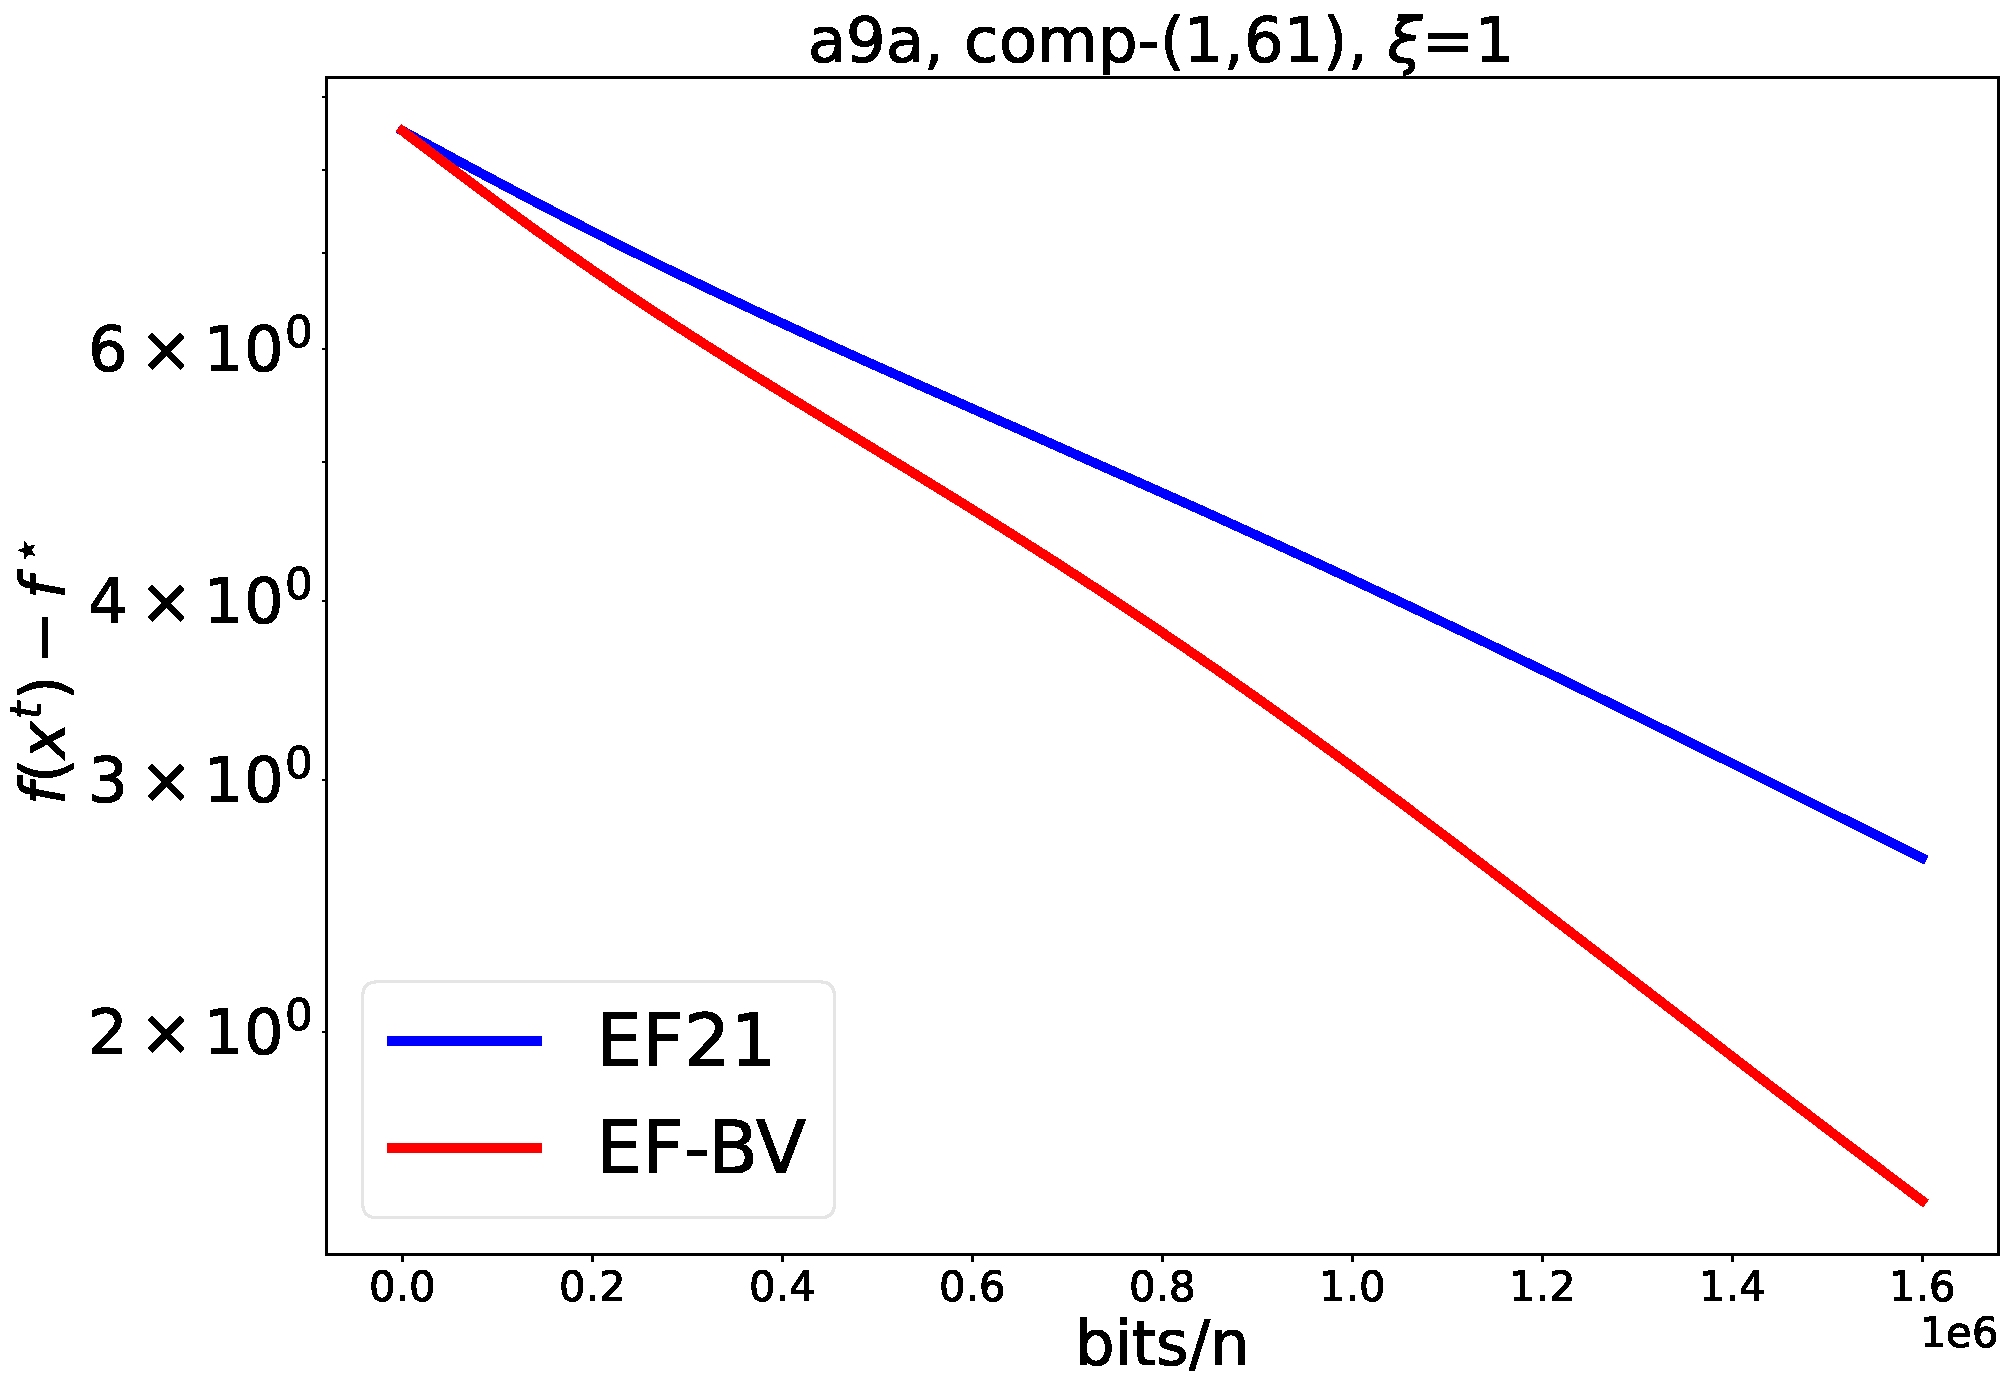
\includegraphics[width=\textwidth]{img/a9a/CompK_61_1_a9a_8124workers_3000K_32561_a9a_61_1_1_1_logreg_diff_conv.pdf}
         % \caption{no partial participation}
         \label{001}
      \end{subfigure}
      \hfill
      \begin{subfigure}[b]{0.32\textwidth}
         \centering
         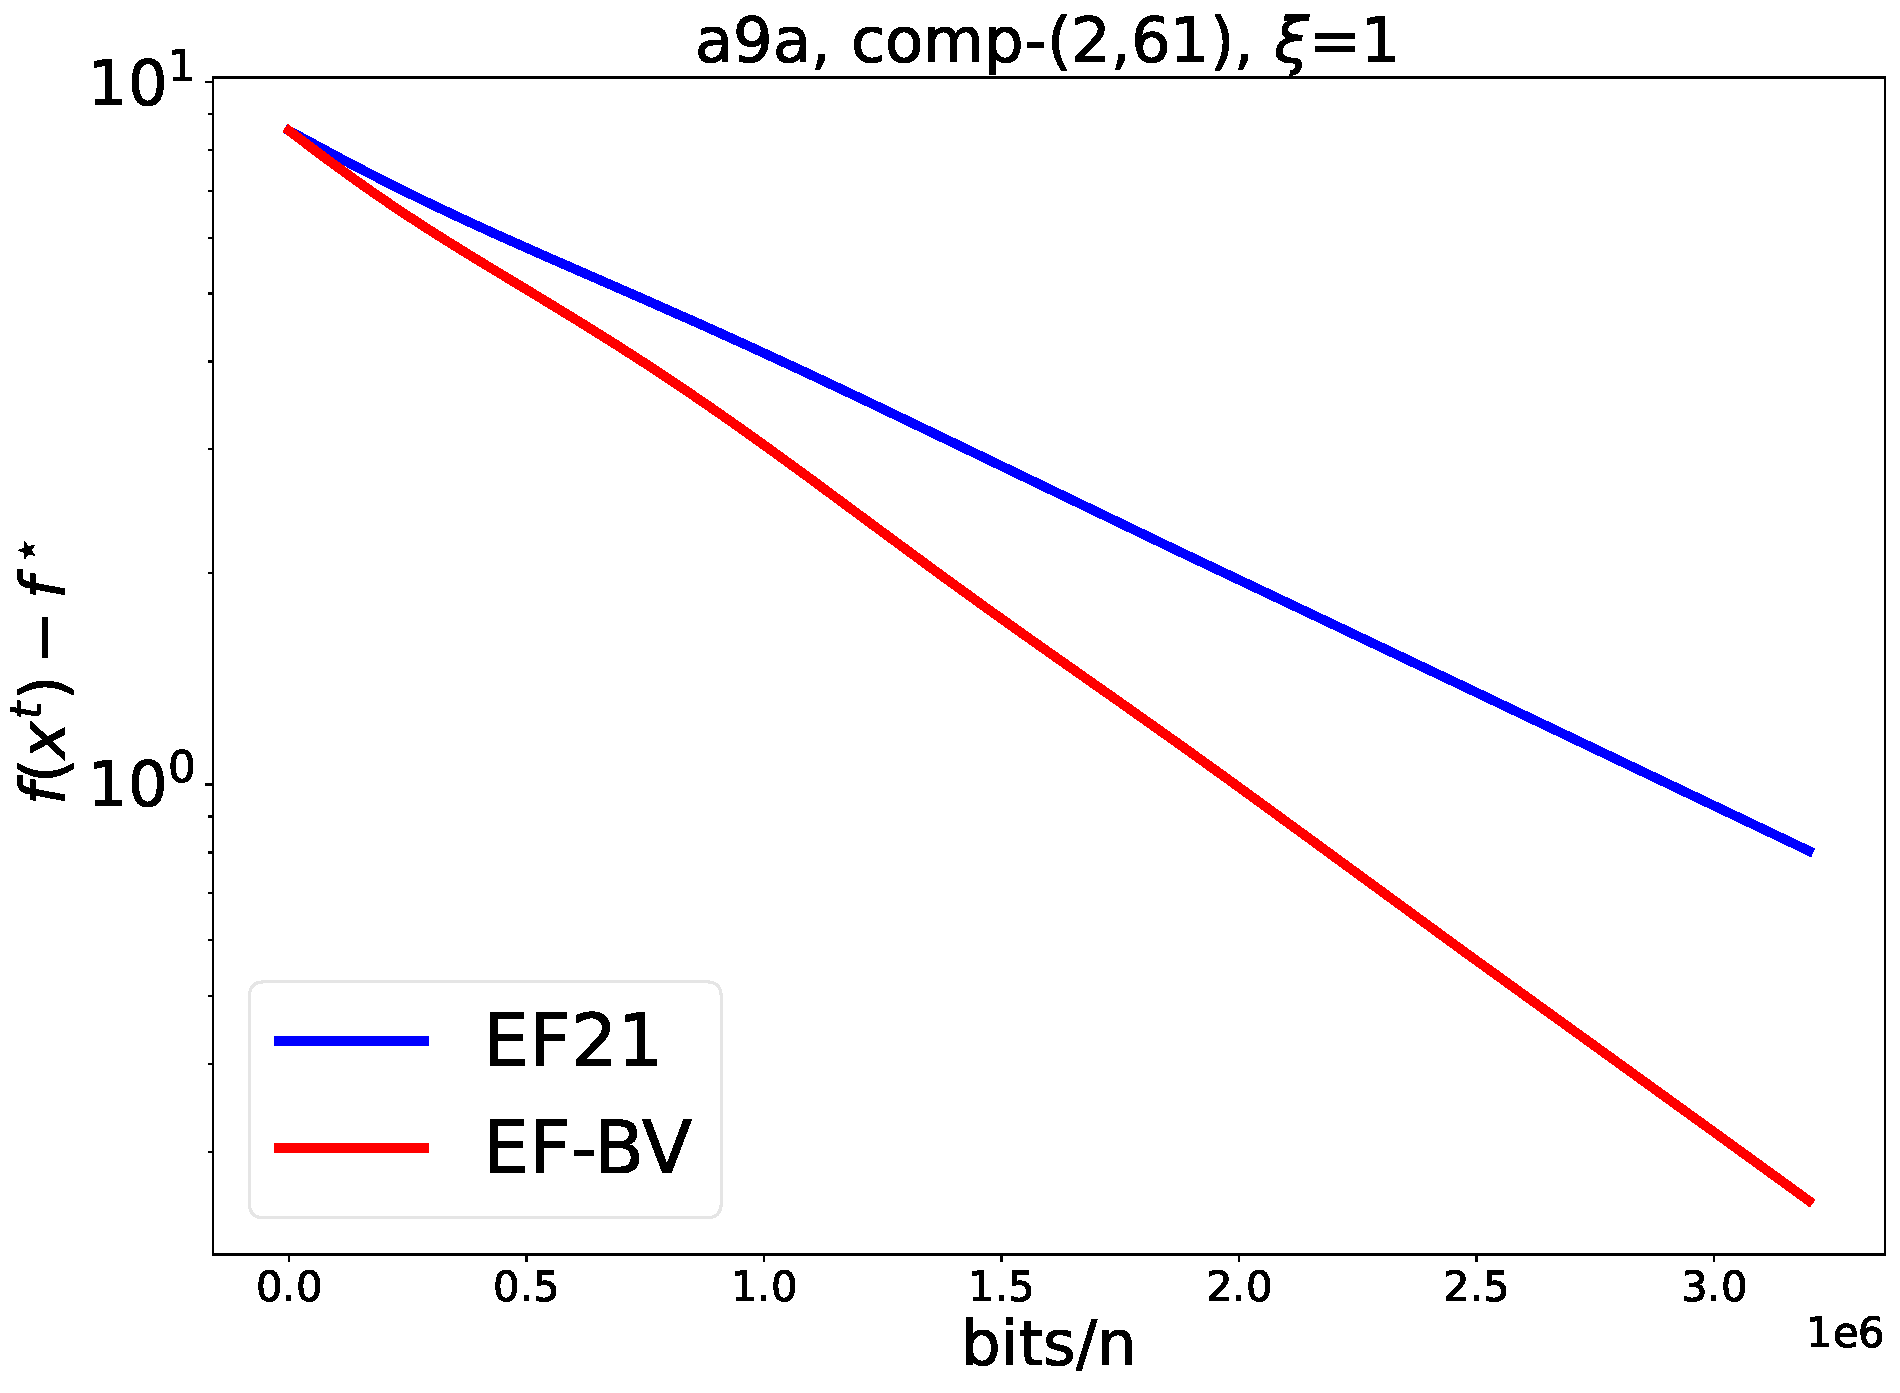
\includegraphics[width=\textwidth]{img/a9a/CompK_61_2_a9a_8124workers_3000K_32561_a9a_61_2_1_1_logreg_diff_conv.pdf}
         % \caption{no partial participation}
         \label{002}
      \end{subfigure}
      \hfill
      \begin{subfigure}[b]{0.32\textwidth}
         \centering
         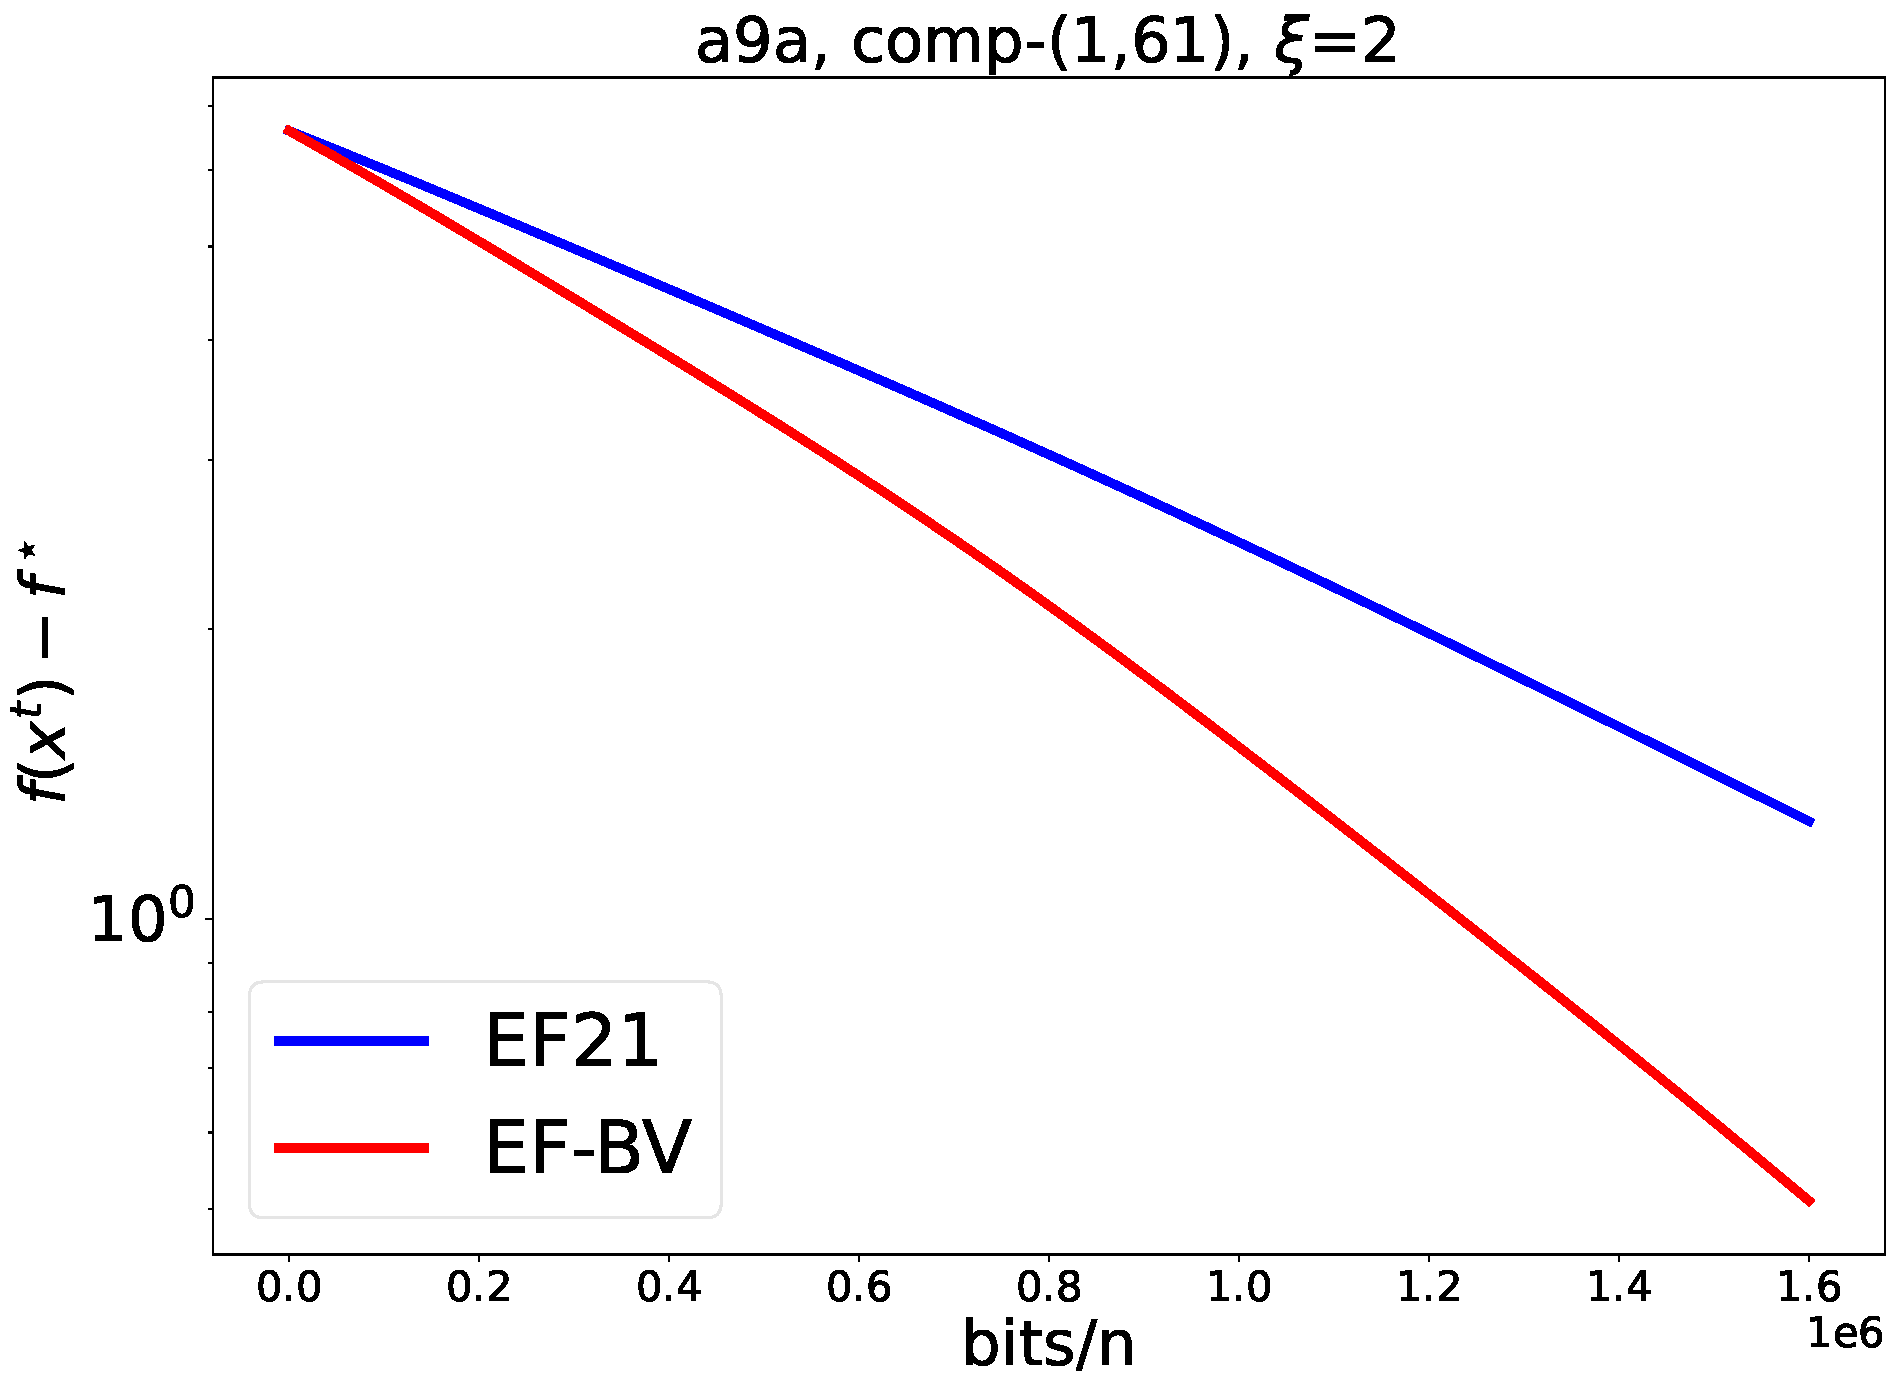
\includegraphics[width=\textwidth]{img/a9a/CompK_61_1_a9a_8124workers_3000K_32561_a9a_61_1_1_2_logreg_diff_conv.pdf}
         % \caption{$\tau=1, lrr=0.1, pr=0.2$}
         \label{003}
      \end{subfigure}
      \hfill
      \begin{subfigure}[b]{0.32\textwidth}
         \centering
         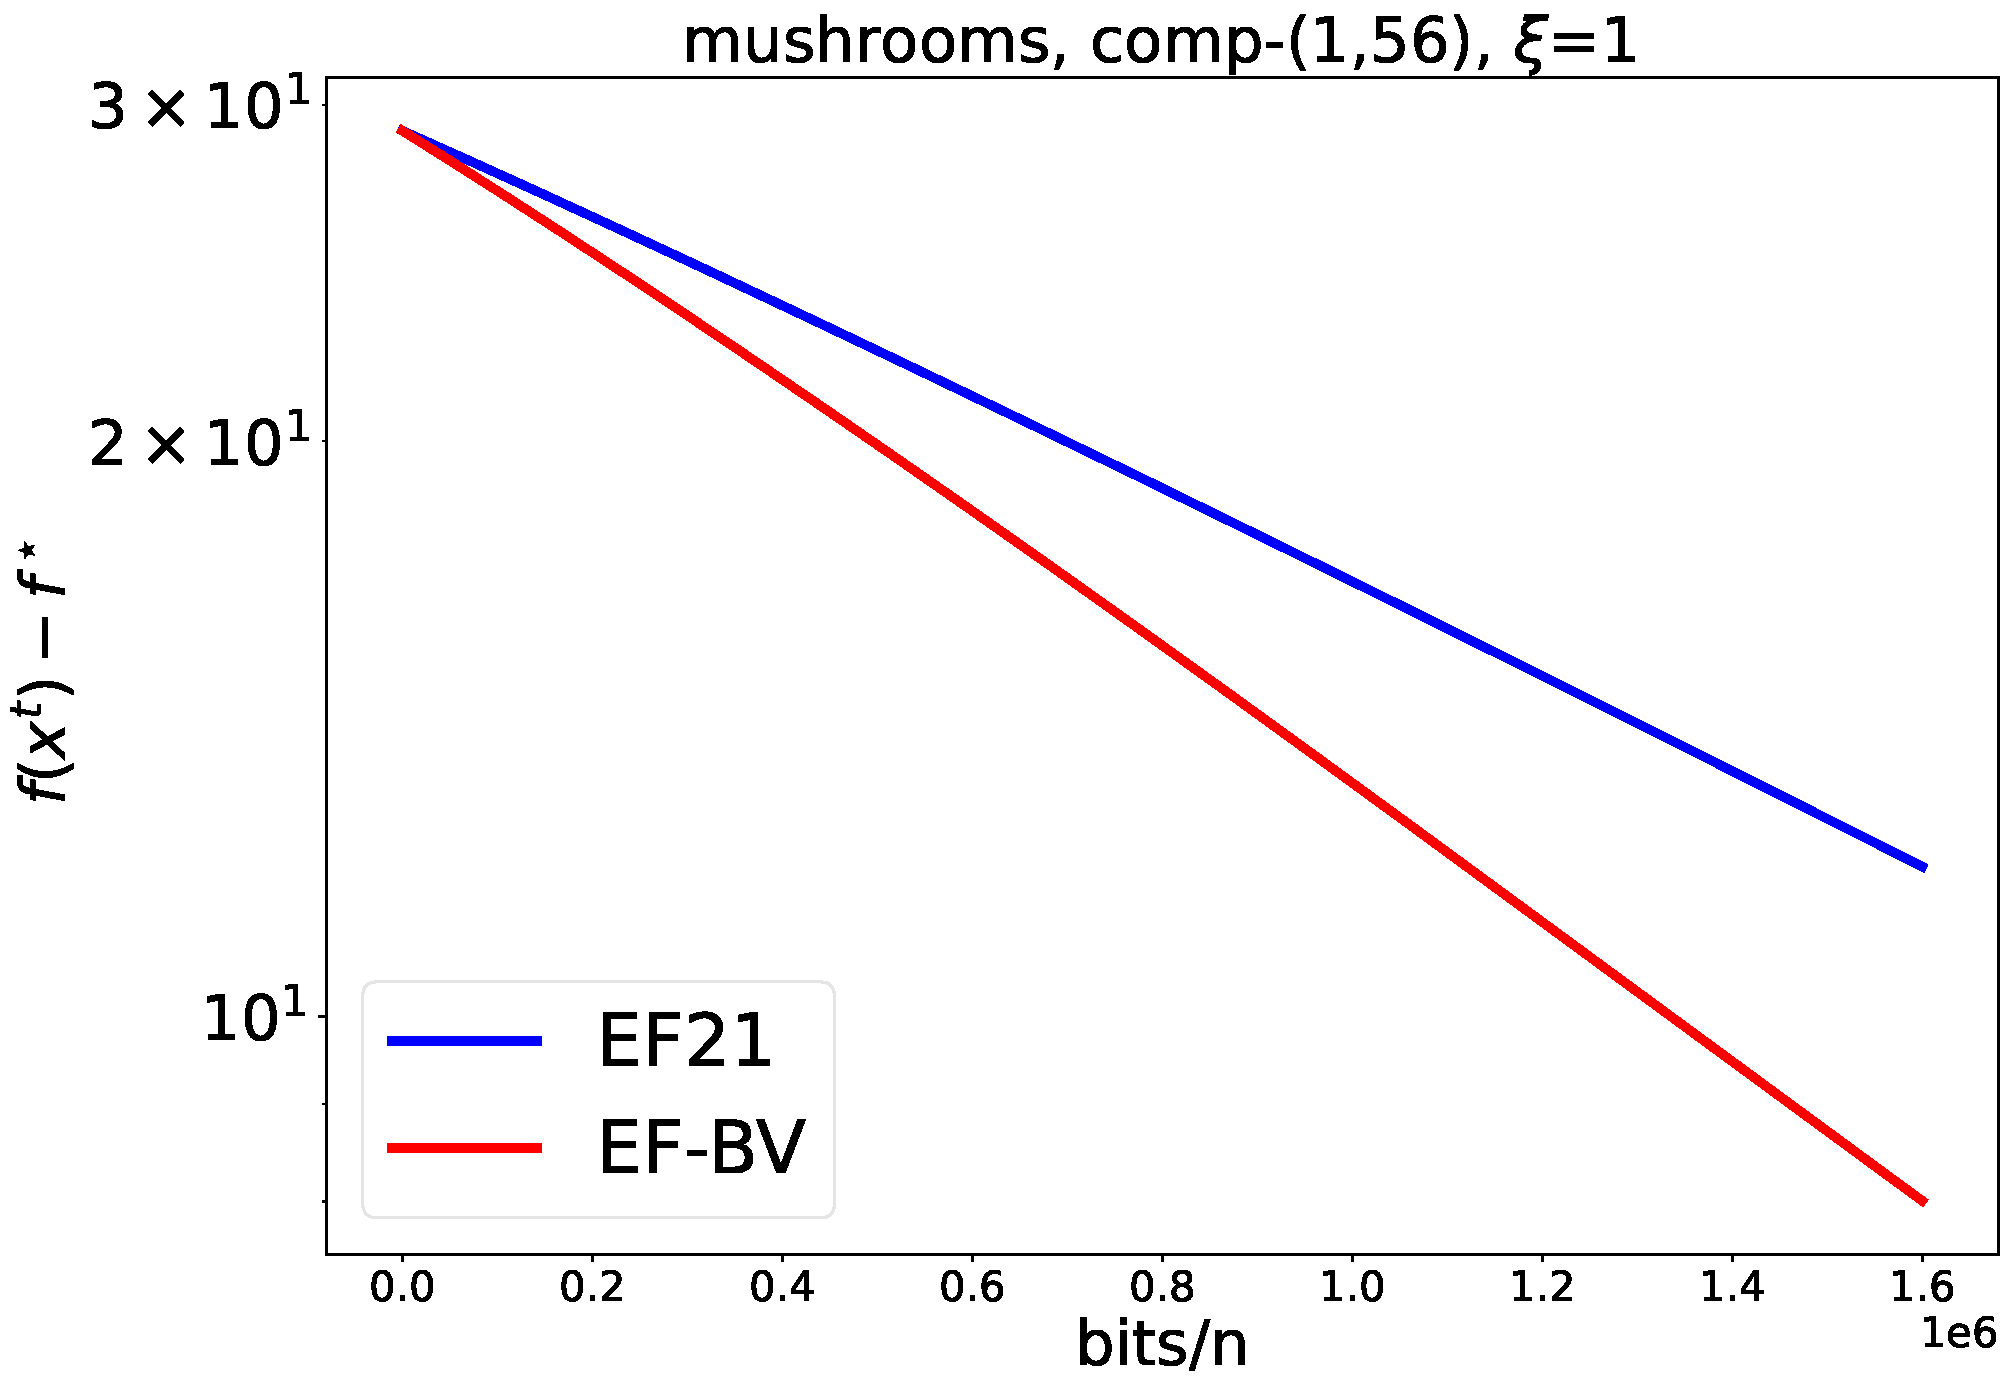
\includegraphics[width=\textwidth]{img/mushrooms/CompK_56_1_mushrooms_8124workers_3000K_8124_mushrooms_56_1_1_1_logreg_diff_conv.pdf}
         % \caption{no partial participation}
         \label{004}
      \end{subfigure}
      \hfill
      \begin{subfigure}[b]{0.32\textwidth}
         \centering
         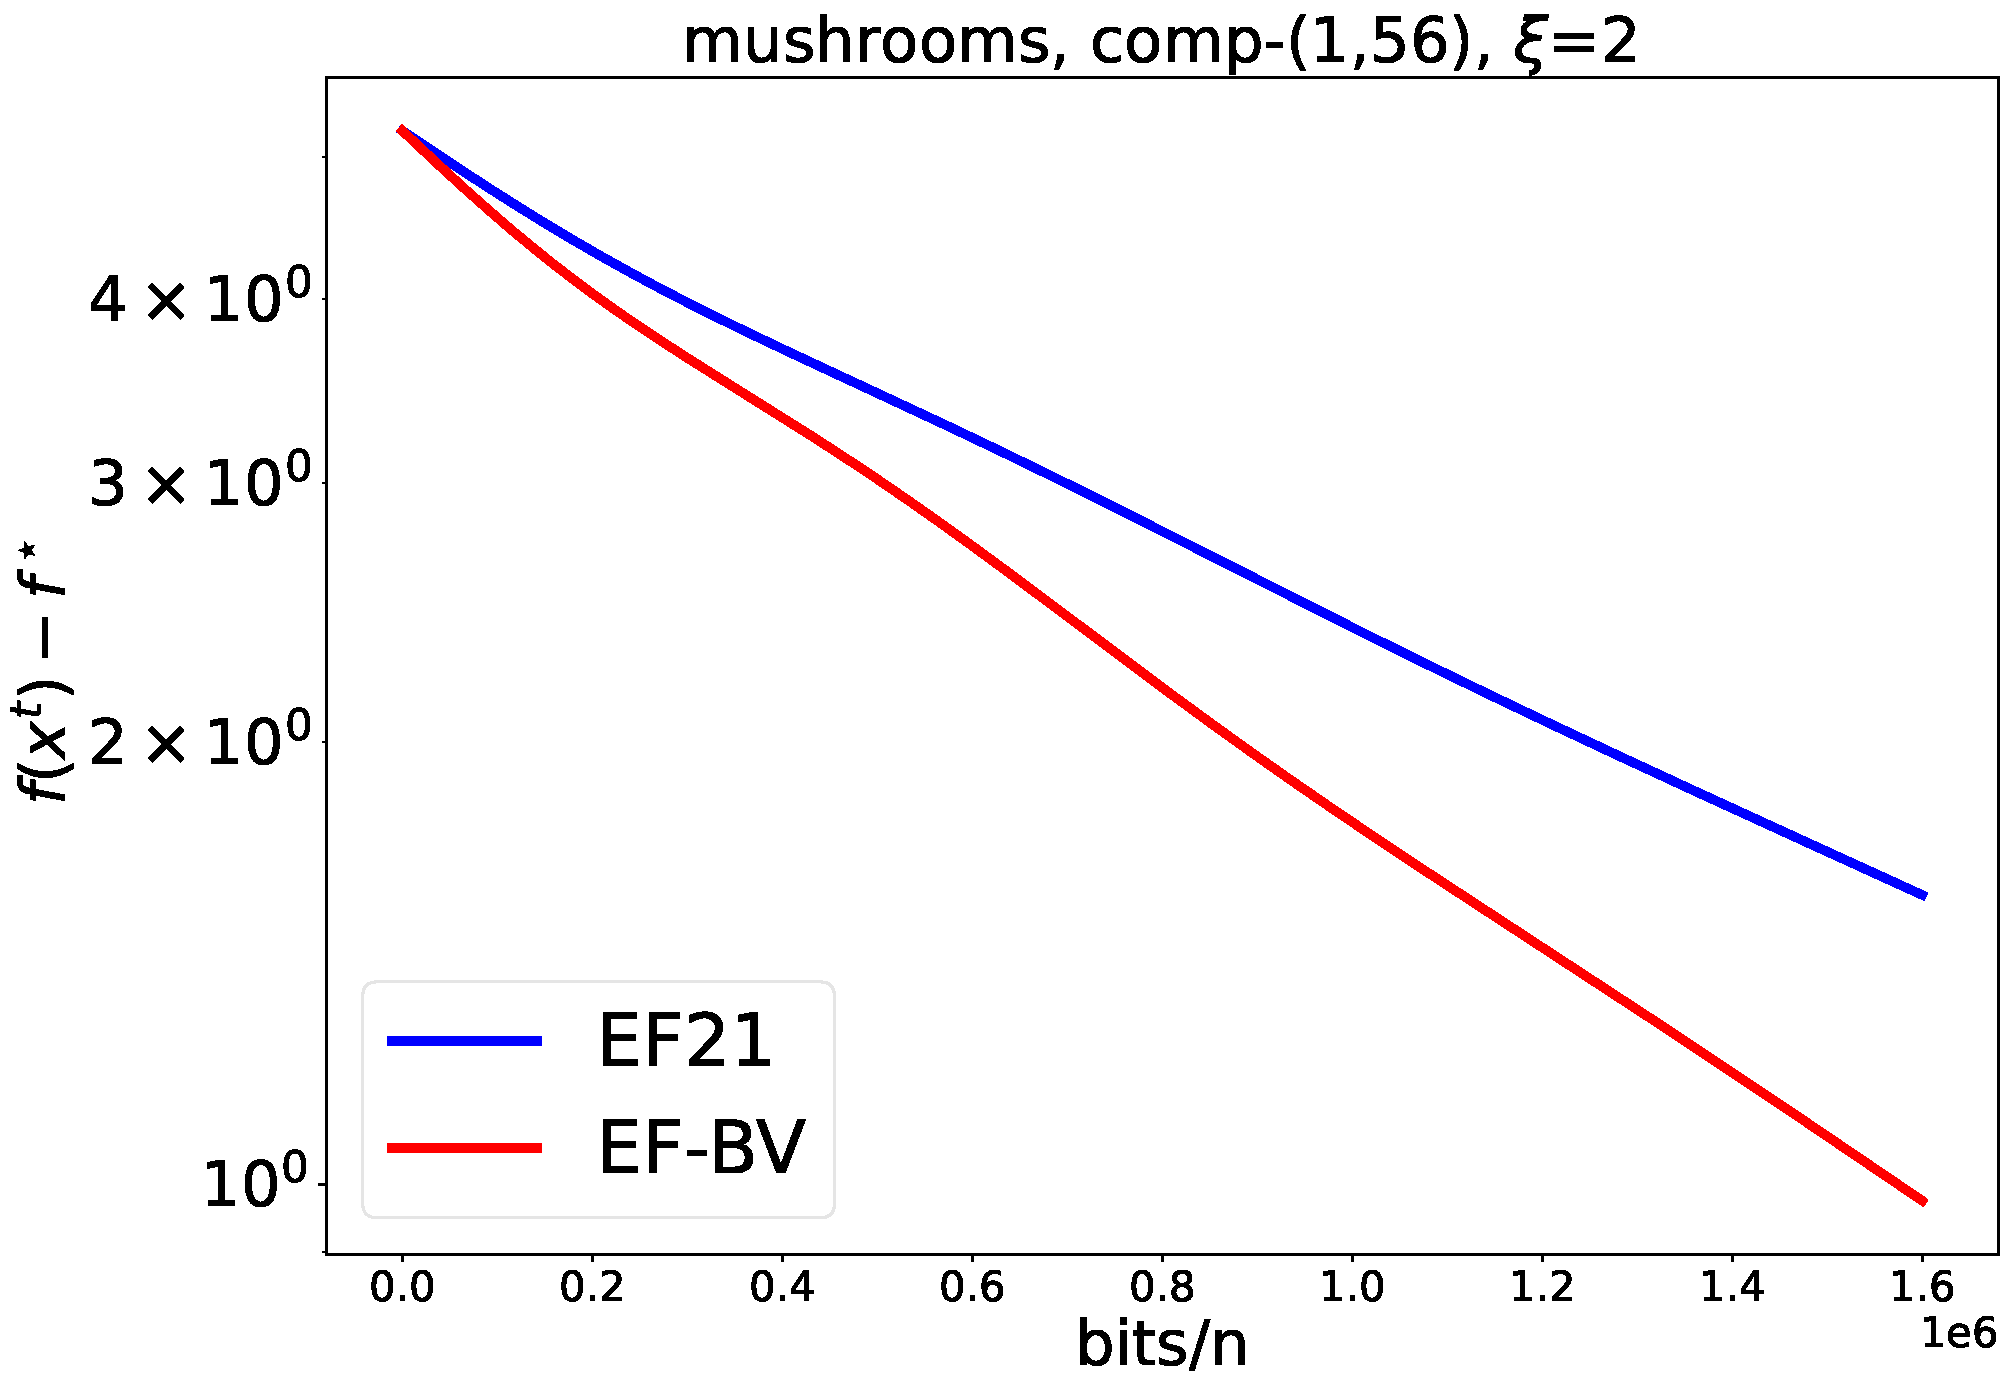
\includegraphics[width=\textwidth]{img/mushrooms/CompK_56_1_mushrooms_8124workers_3000K_8124_mushrooms_56_1_1_2_logreg_diff_conv.pdf}
         % \caption{no partial participation}
         \label{005}
      \end{subfigure}
      \hfill
      \begin{subfigure}[b]{0.32\textwidth}
         \centering
         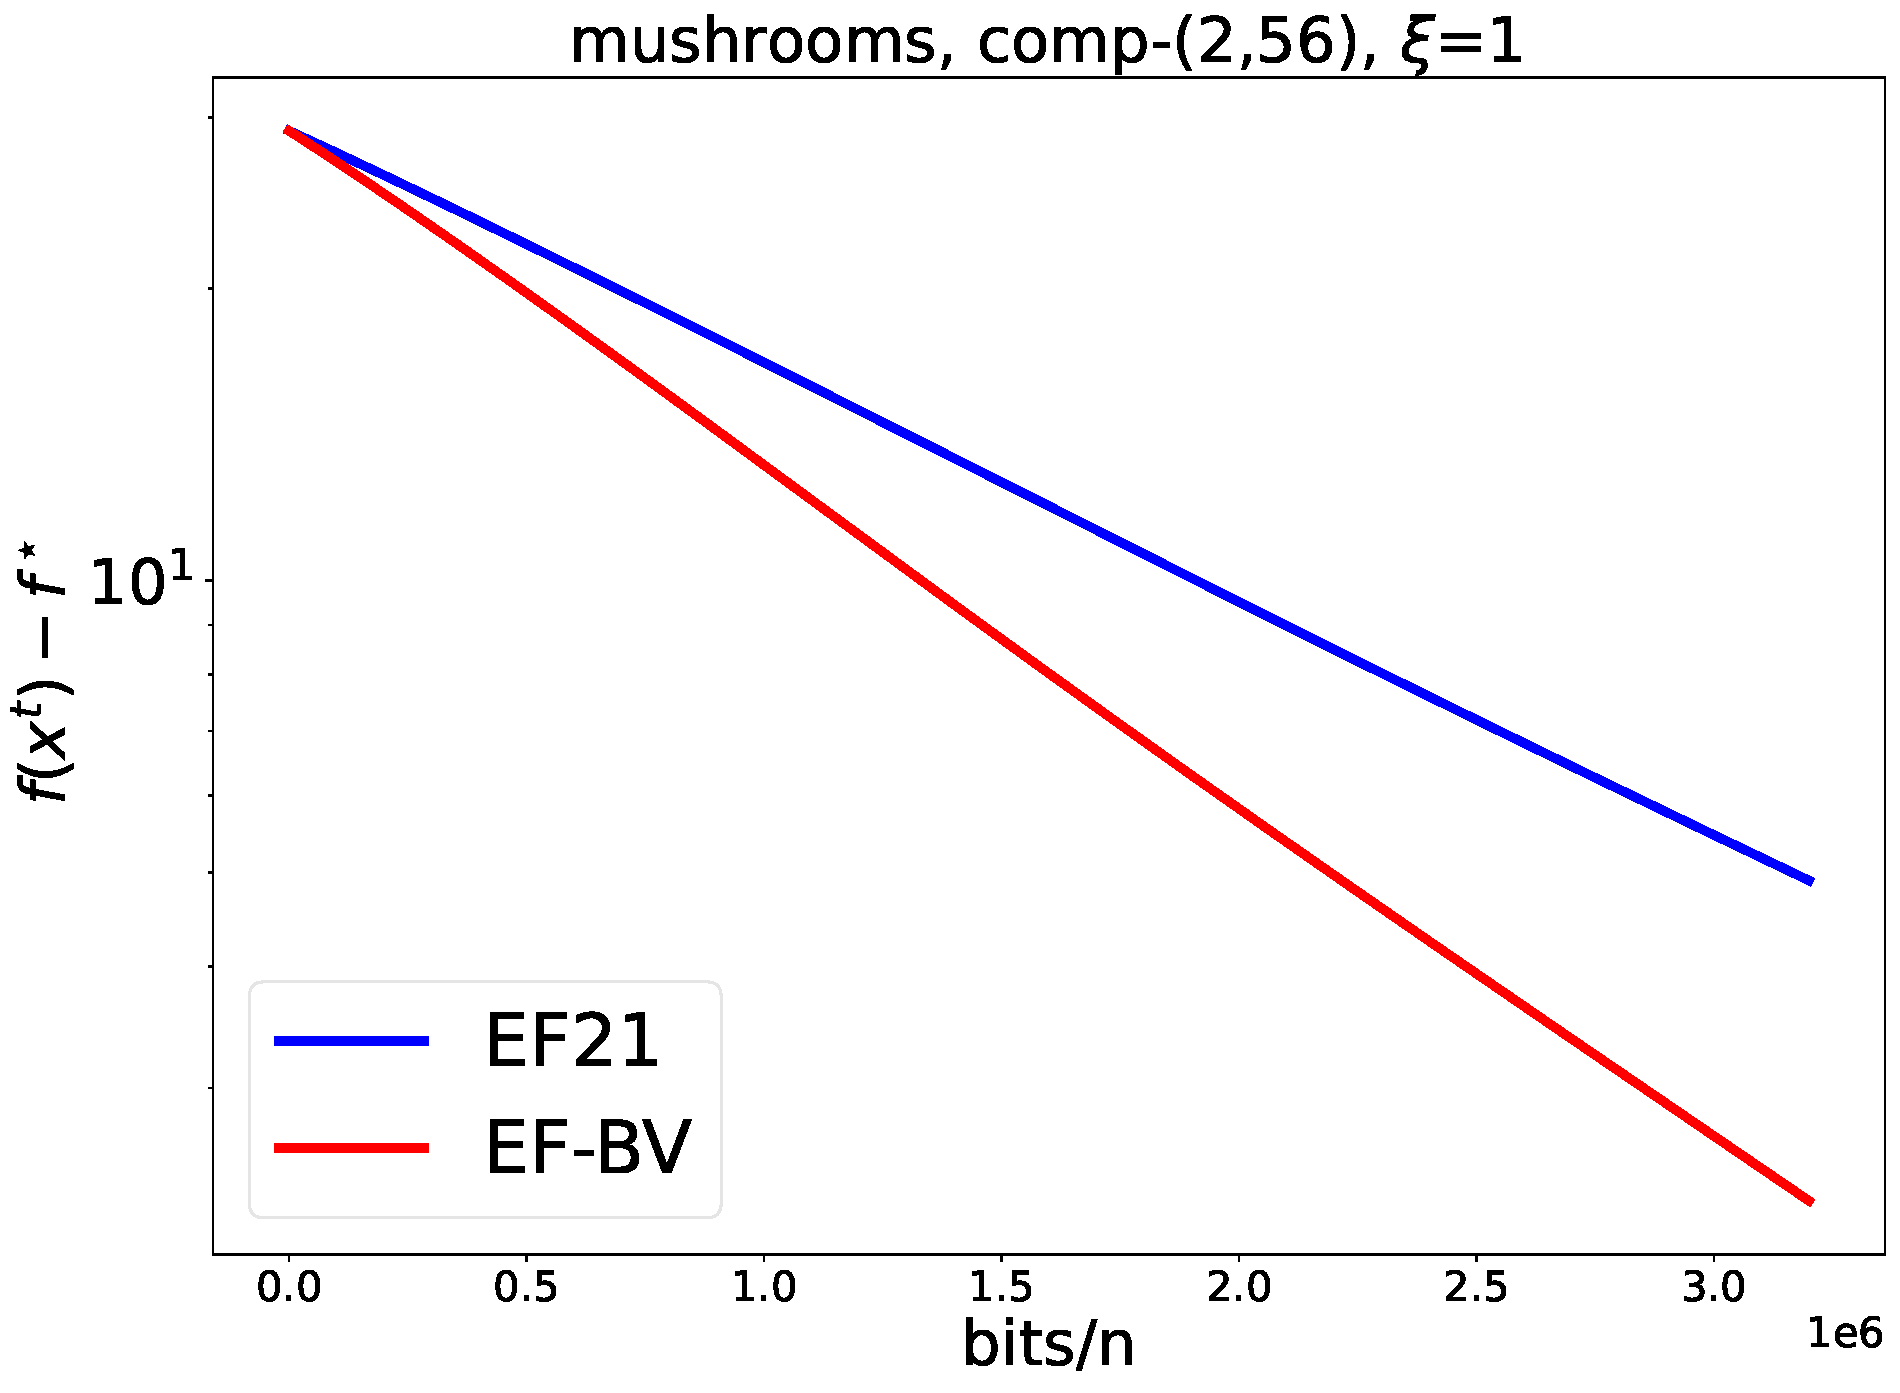
\includegraphics[width=\textwidth]{img/mushrooms/CompK_56_2_mushrooms_8124workers_3000K_8124_mushrooms_56_2_1_1_logreg_diff_conv.pdf}
         % \caption{$\tau=1, lrr=0.1, pr=0.2$}
         \label{006}
      \end{subfigure}
      \hfill
      \begin{subfigure}[b]{0.32\textwidth}
         \centering
         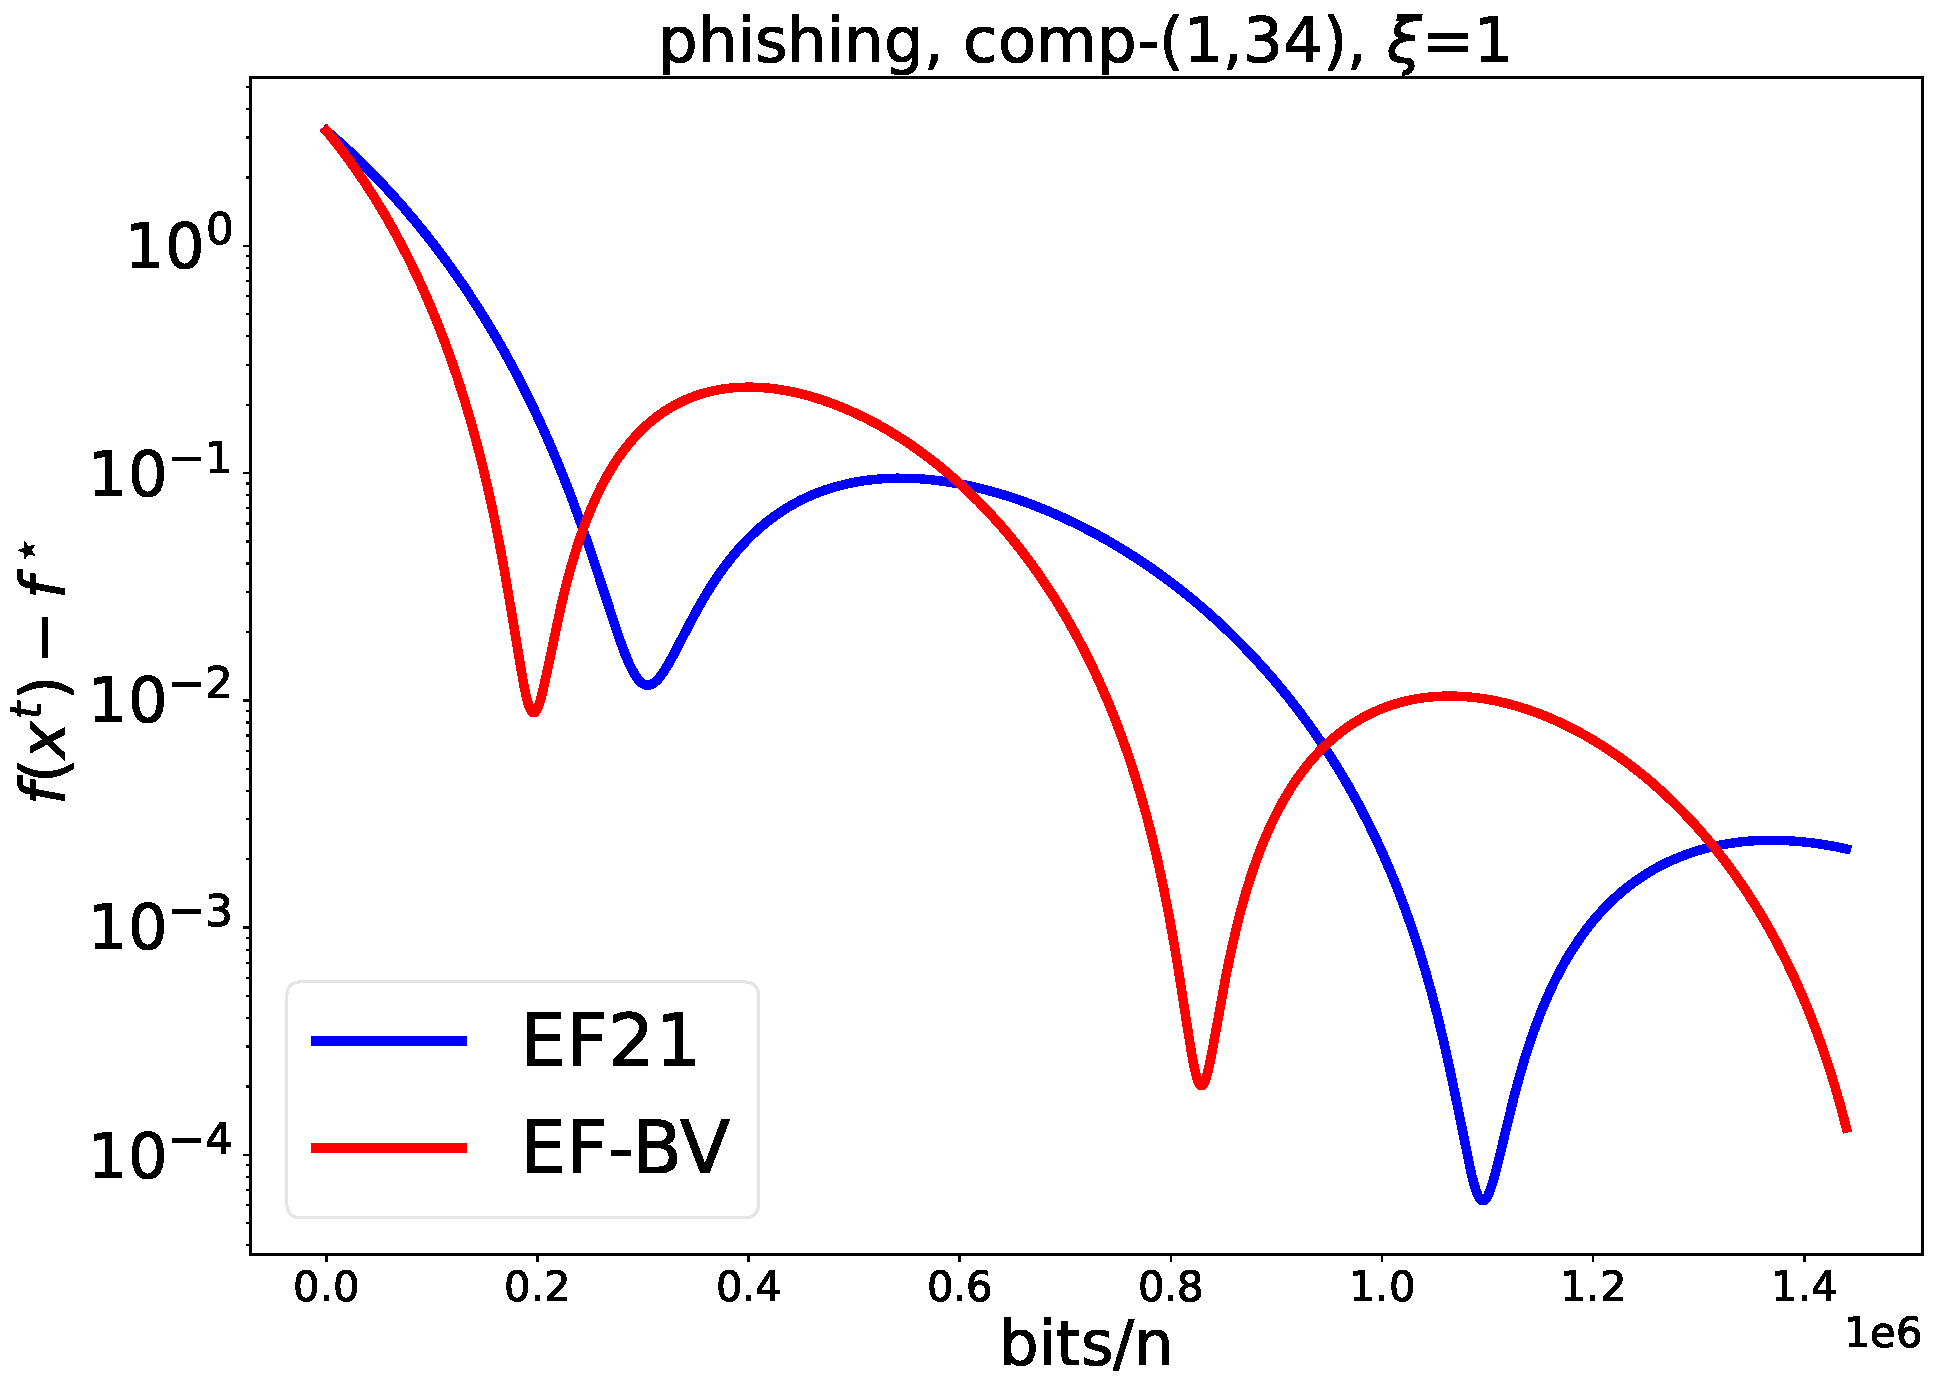
\includegraphics[width=\textwidth]{img/phishing/CompK_34_1_phishing_8124workers_3000K_11055_phishing_34_1_1_1_logreg_diff_conv.pdf}
         % \caption{no partial participation}
         \label{007}
      \end{subfigure}
      \hfill
      \begin{subfigure}[b]{0.32\textwidth}
         \centering
         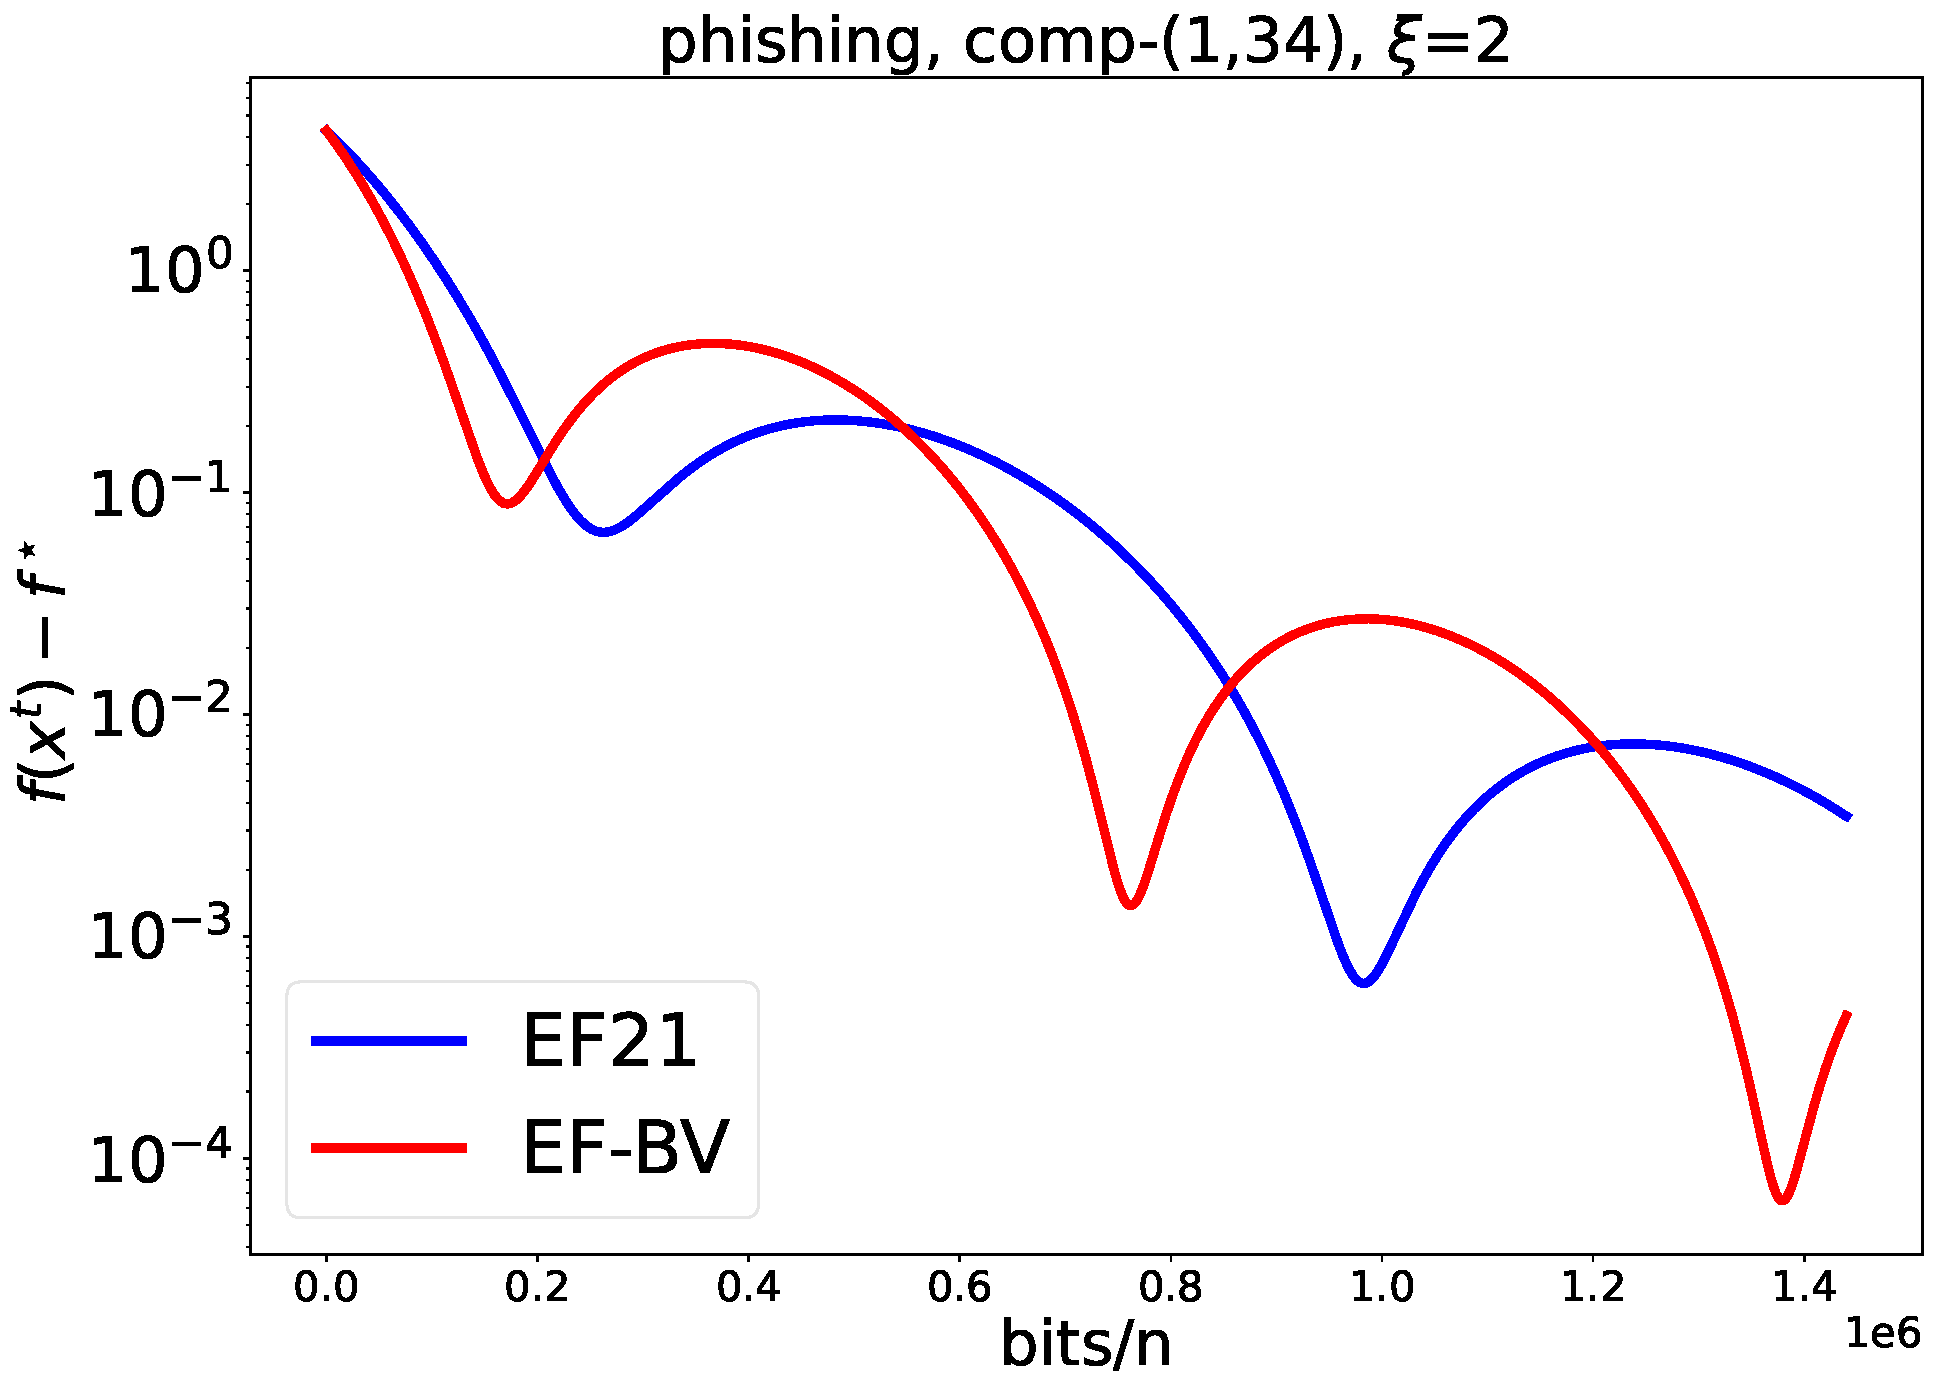
\includegraphics[width=\textwidth]{img/phishing/CompK_34_1_phishing_8124workers_3000K_11055_phishing_34_1_1_2_logreg_diff_conv.pdf}
         % \caption{no partial participation}
         \label{008}
      \end{subfigure}
      \hfill
      \begin{subfigure}[b]{0.32\textwidth}
         \centering
         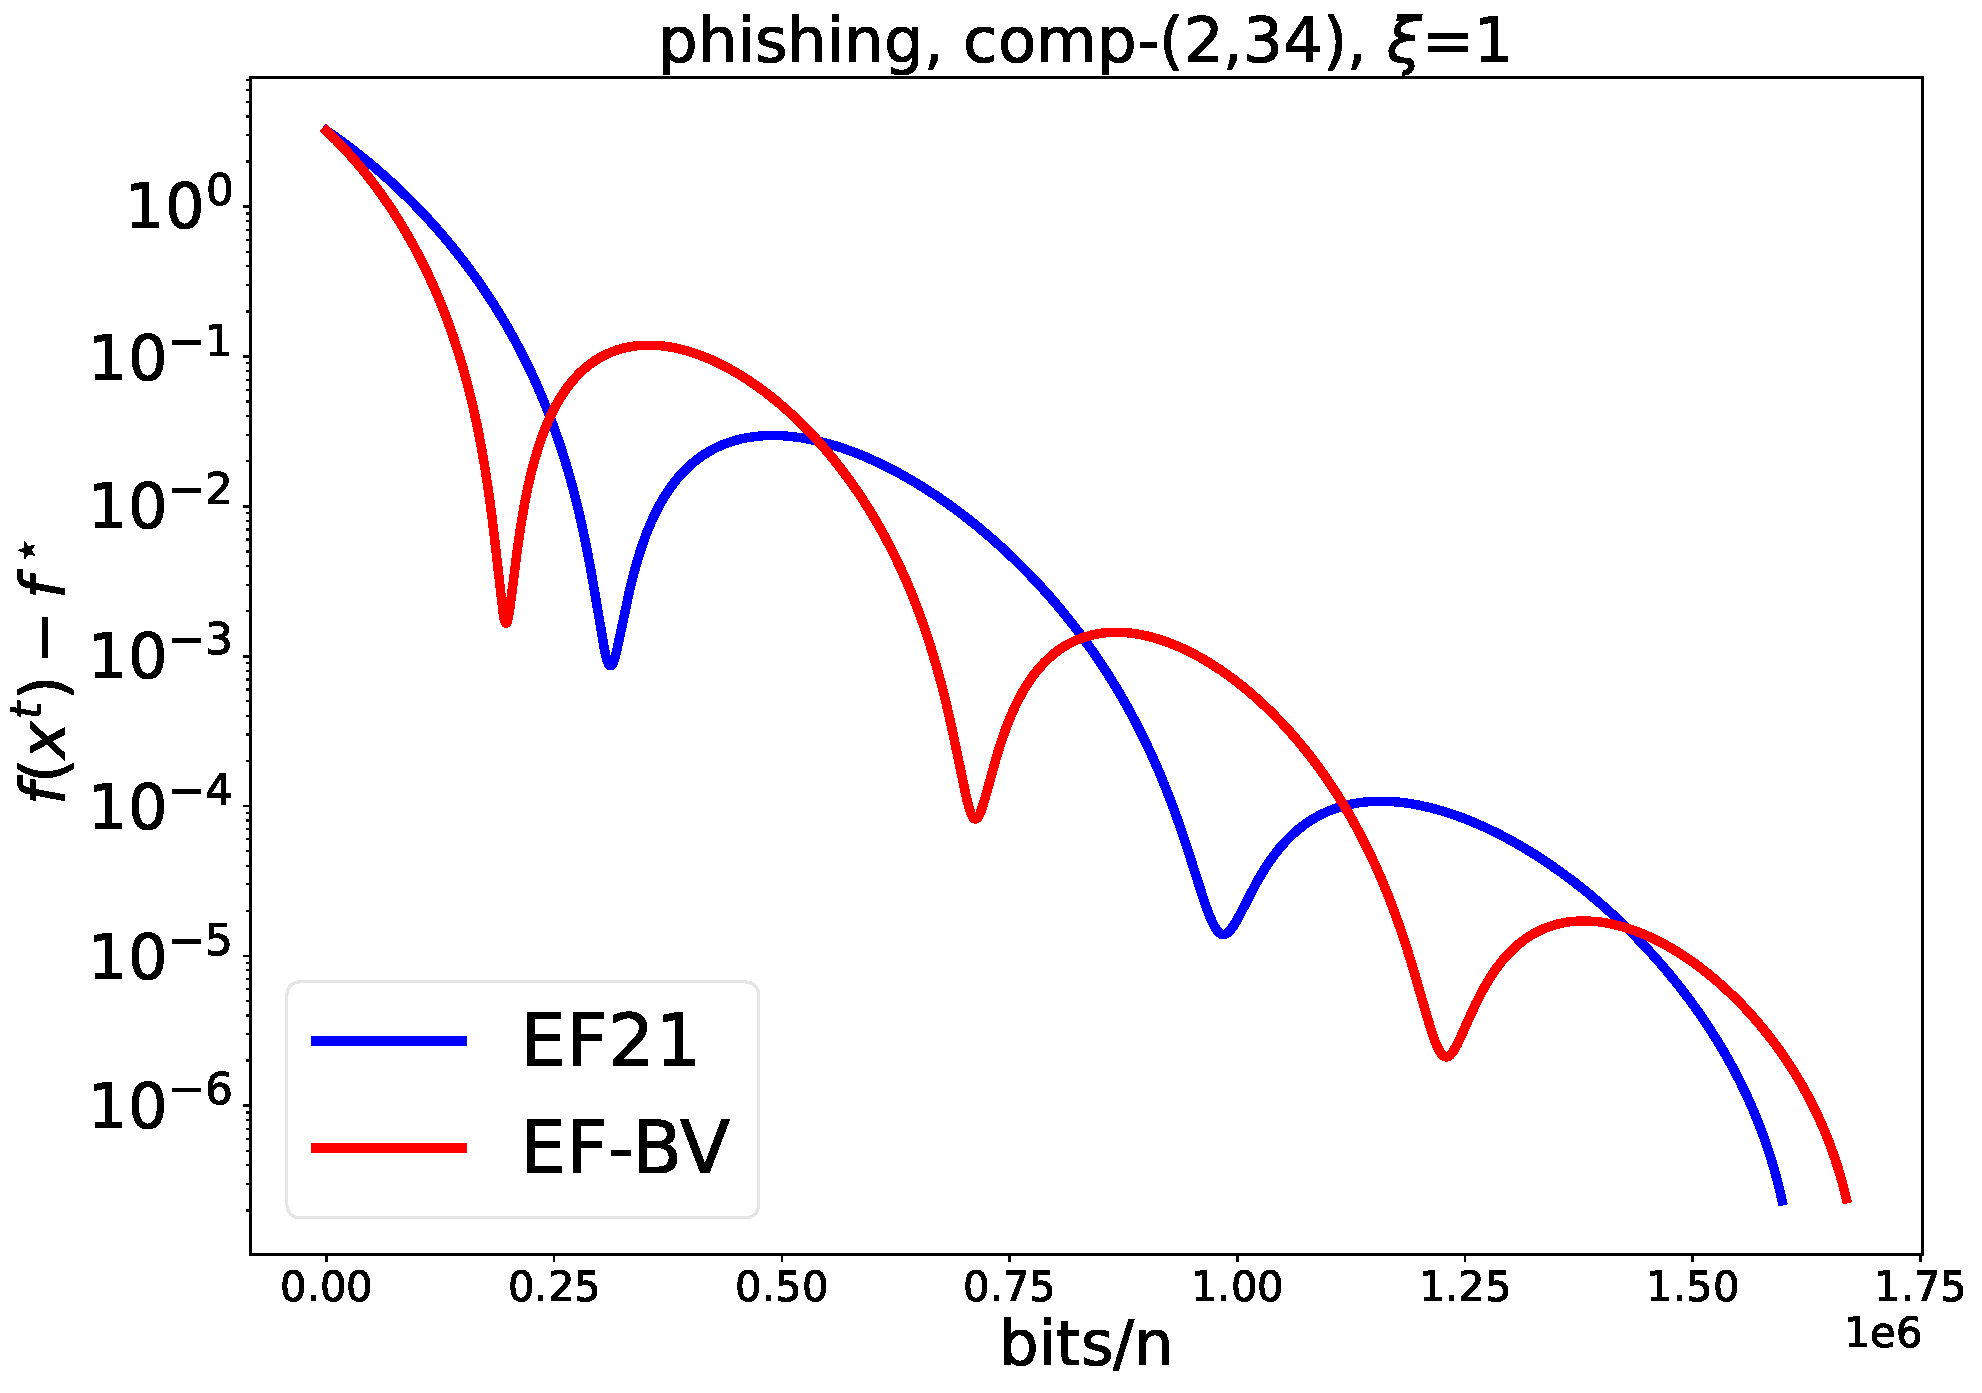
\includegraphics[width=\textwidth]{img/phishing/CompK_34_2_phishing_8124workers_3000K_11055_phishing_34_2_1_1_logreg_diff_conv.pdf}
         % \caption{$\tau=1, lrr=0.1, pr=0.2$}
         \label{009}
      \end{subfigure}
      % \hfill
      % \begin{subfigure}[b]{0.32\textwidth}
      %    \centering
      %    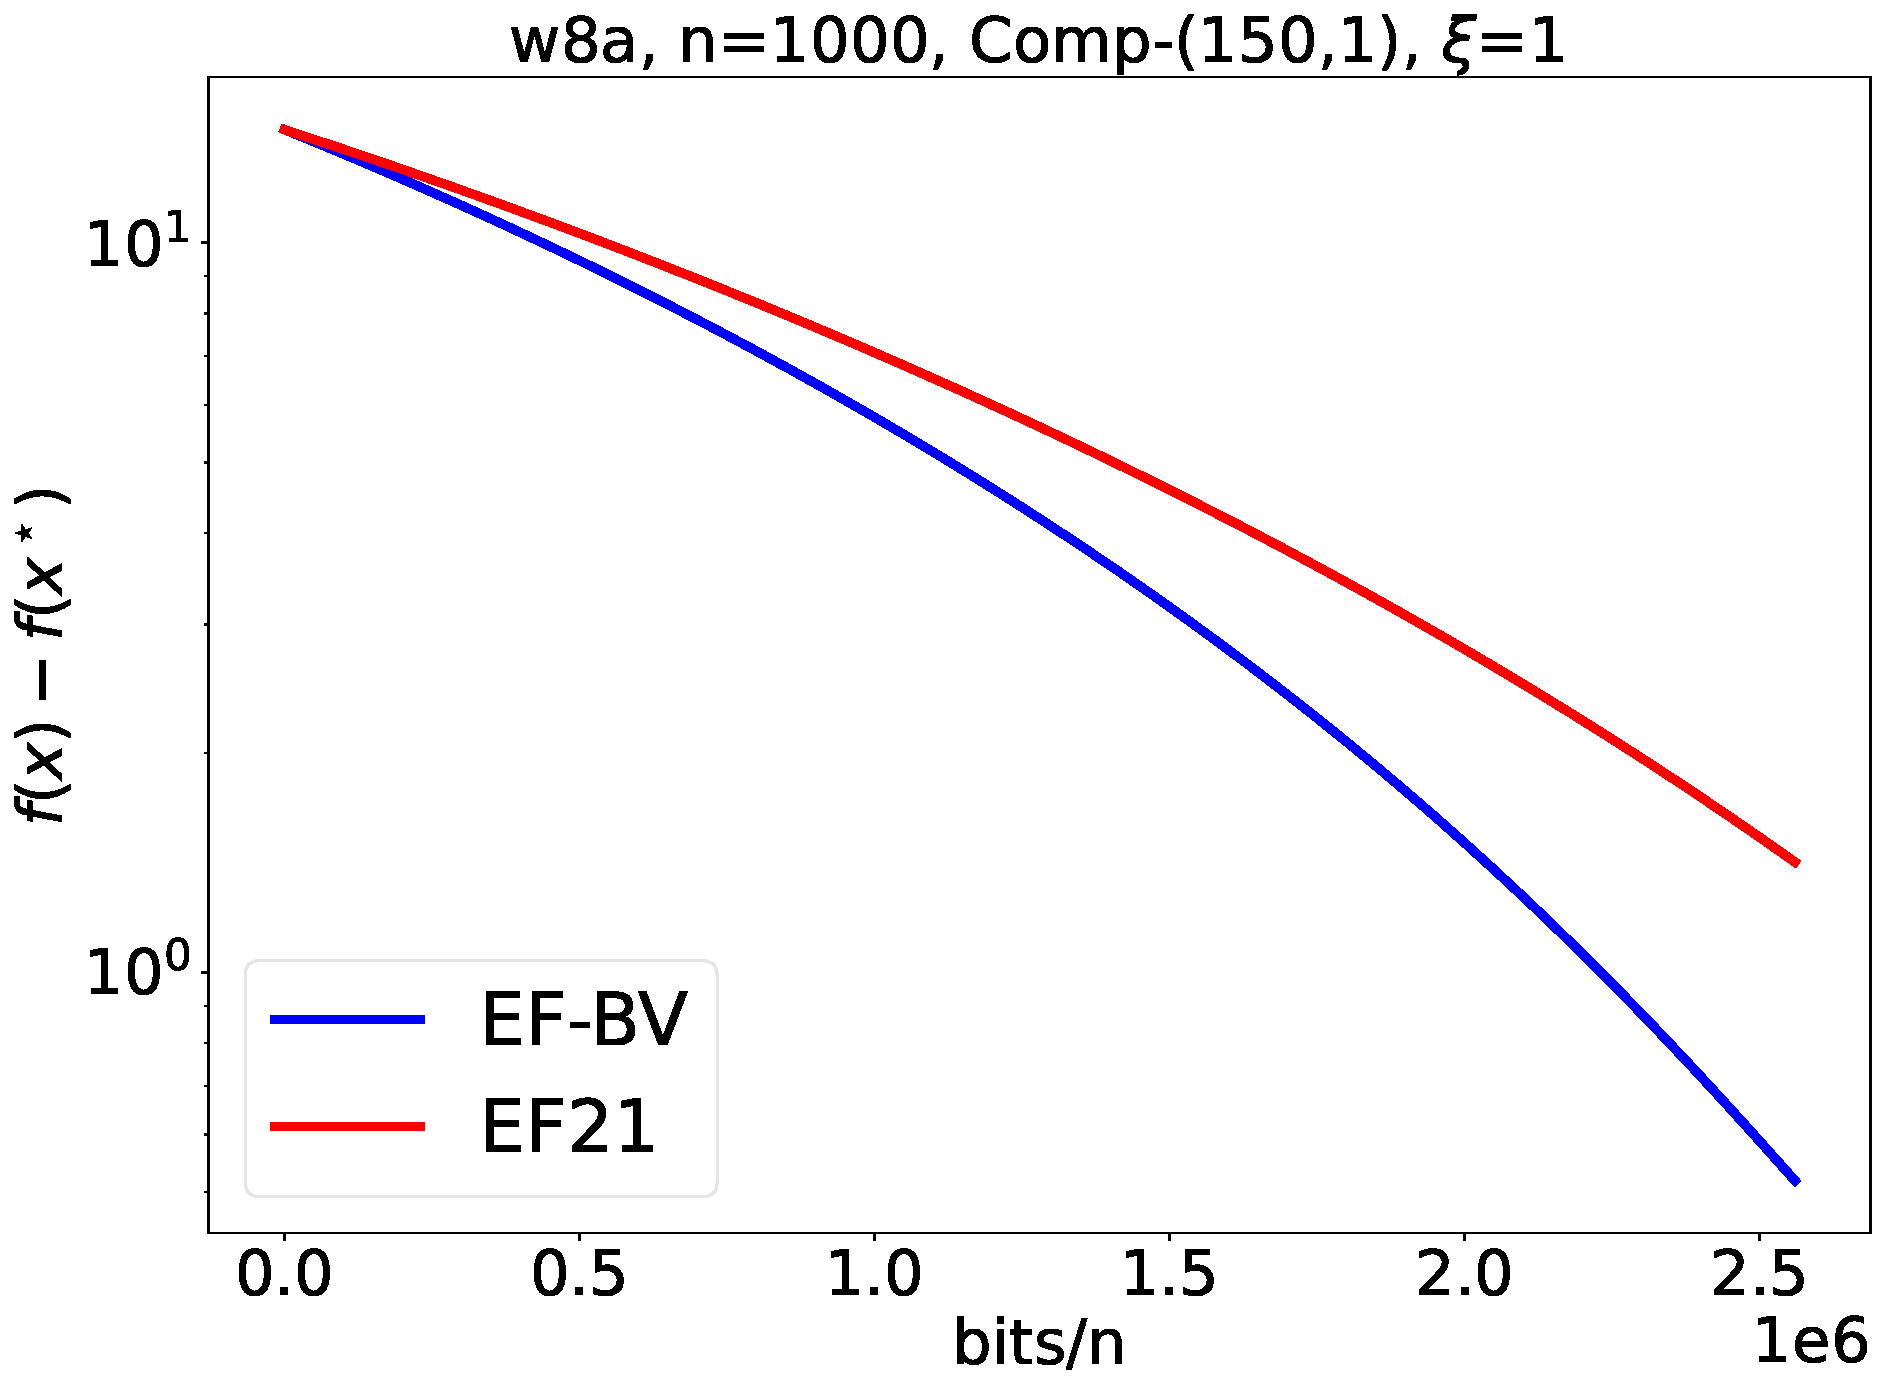
\includegraphics[width=\textwidth]{img/w8a/CompK_150_1_w8a_20workers_3000K_1000_w8a_1_1_logreg_diff.pdf}
      %    % \caption{no partial participation}
      %    \label{010}
      % \end{subfigure}
      % \hfill
      % \begin{subfigure}[b]{0.32\textwidth}
      %    \centering
      %    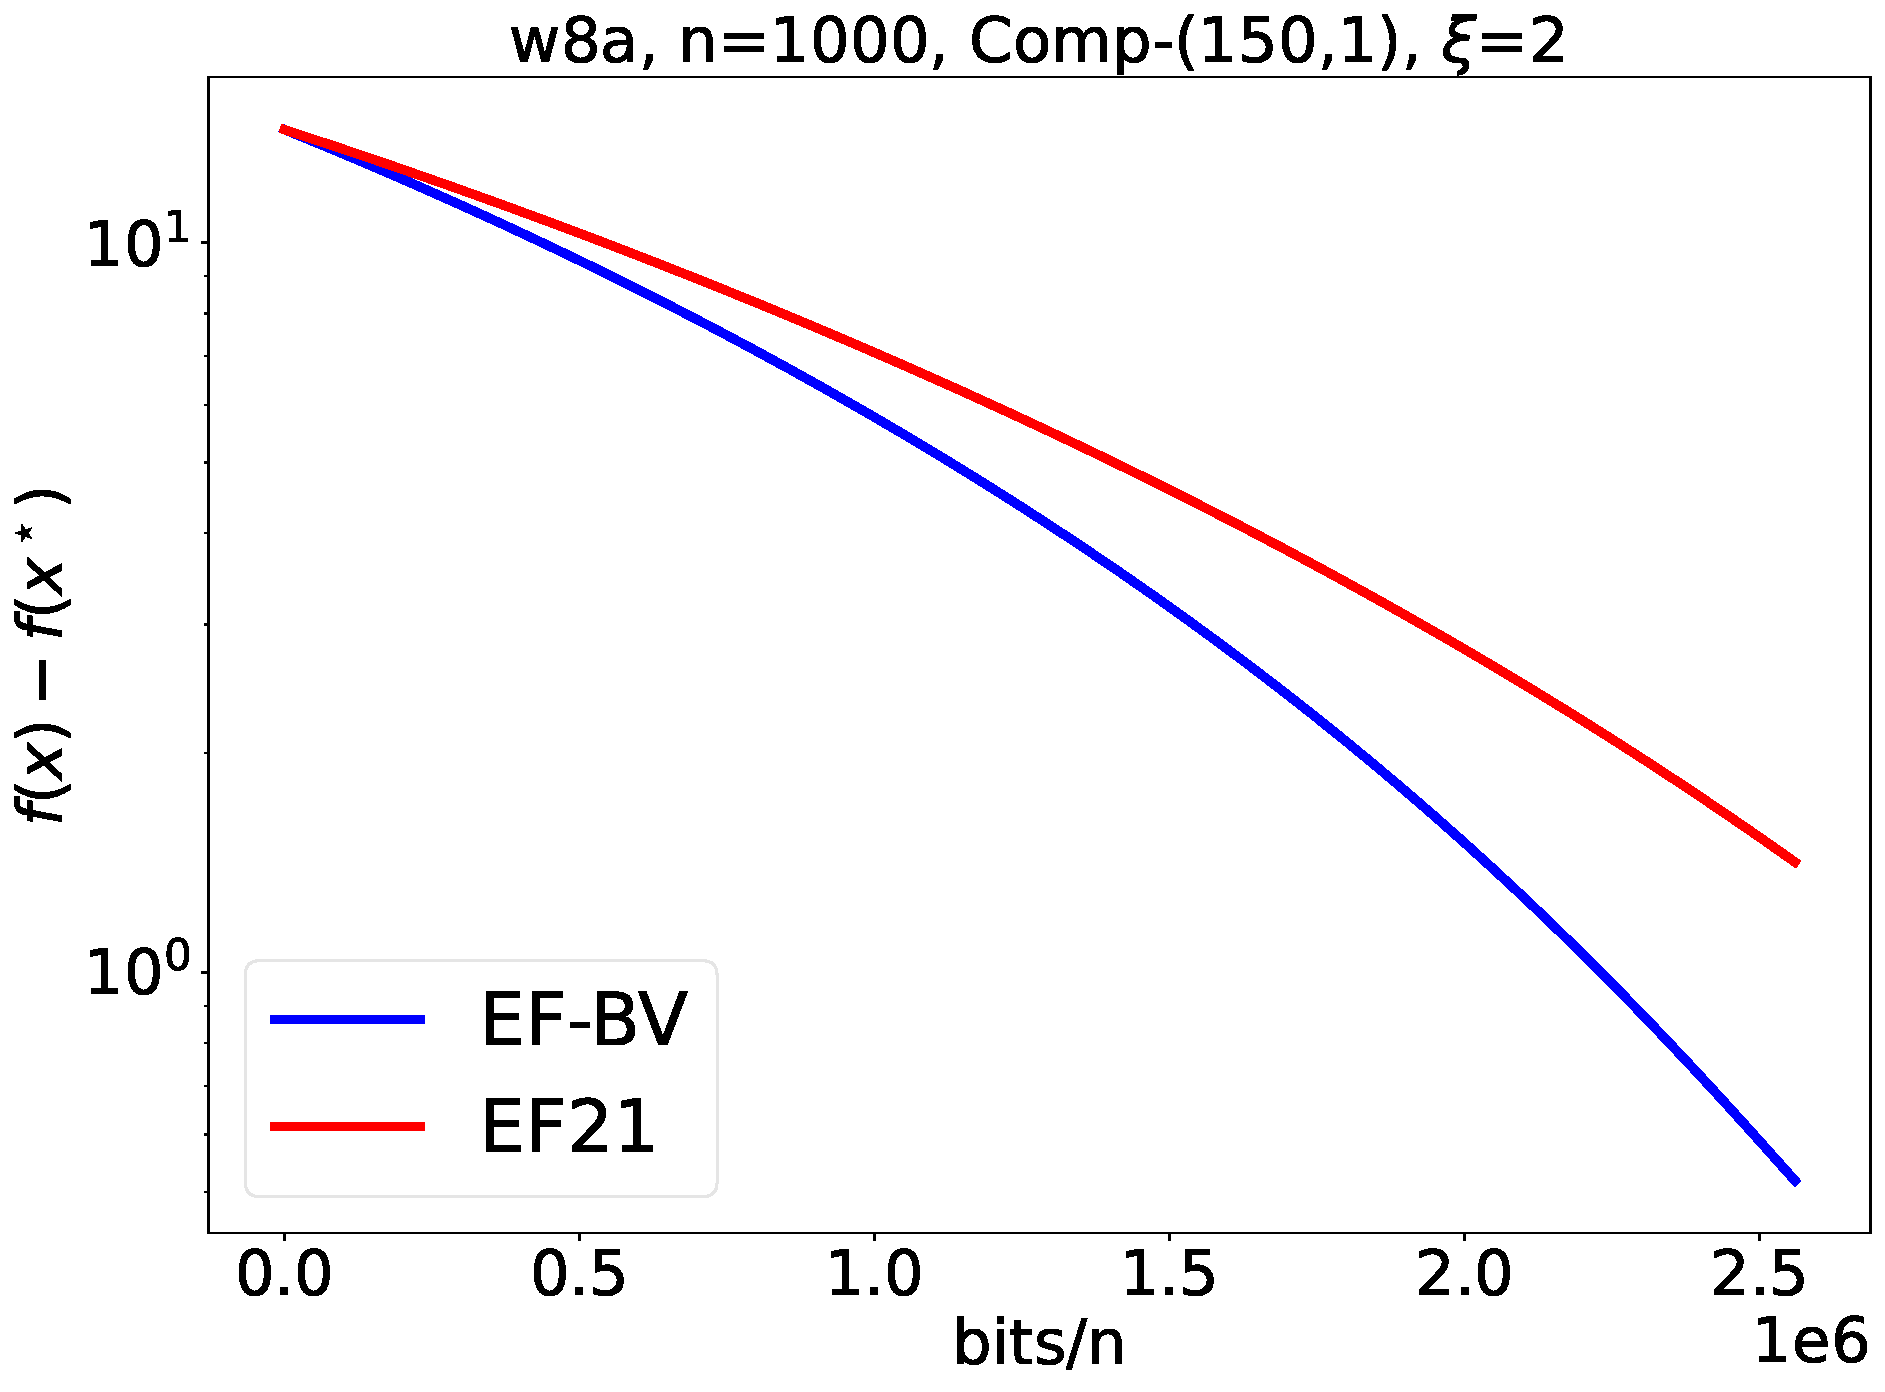
\includegraphics[width=\textwidth]{img/w8a/CompK_150_1_w8a_20workers_3000K_1000_w8a_1_2_logreg_diff.pdf}
      %    % \caption{no partial participation}
      %    \label{011}
      % \end{subfigure}
      % \hfill
      % \begin{subfigure}[b]{0.32\textwidth}
      %    \centering
      %    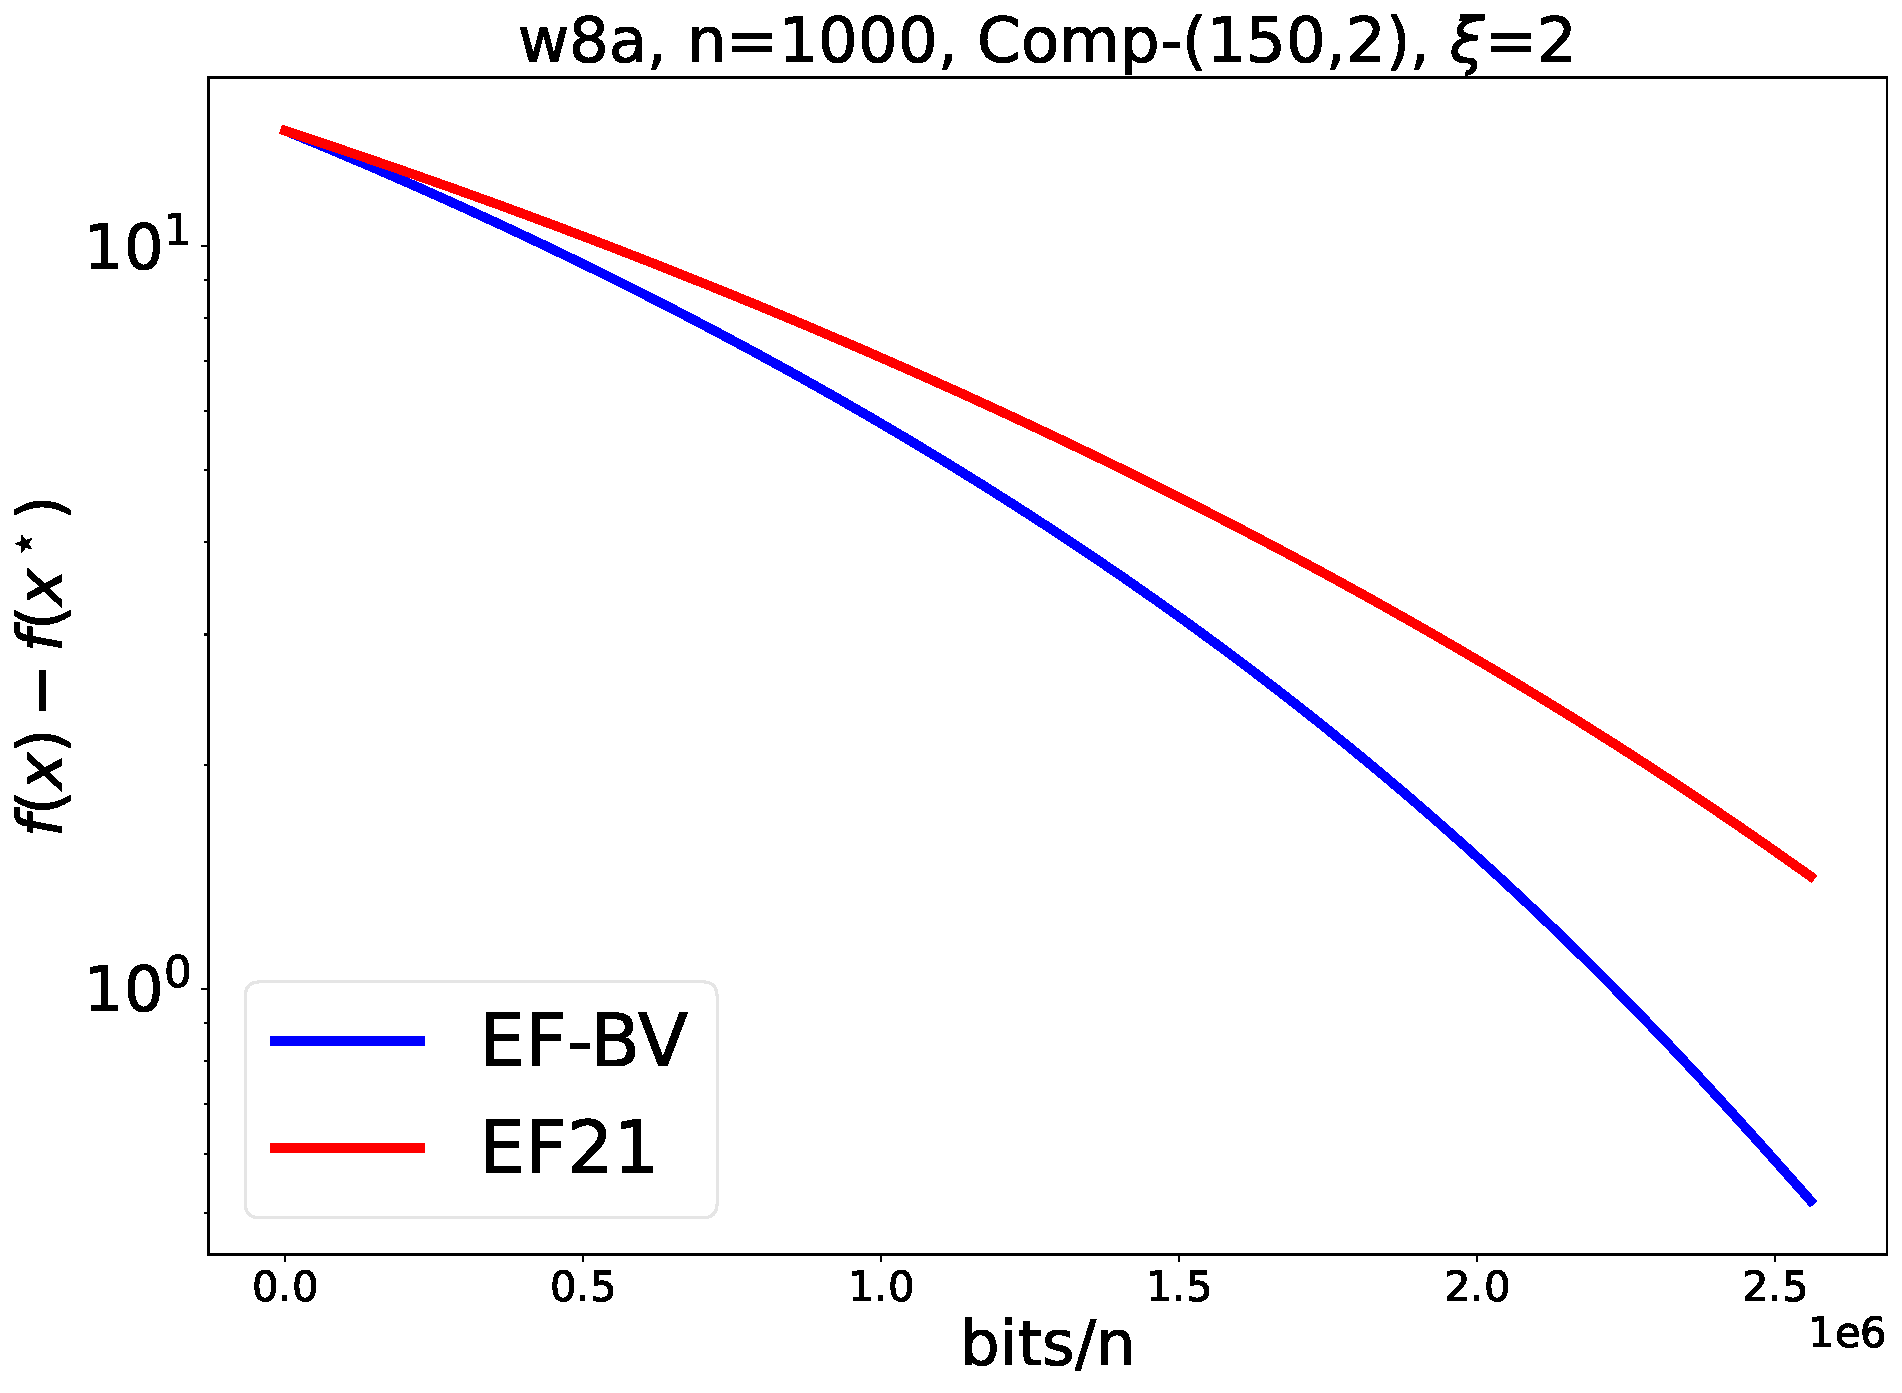
\includegraphics[width=\textwidth]{img/w8a/CompK_150_2_w8a_20workers_3000K_1000_w8a_1_2_logreg_diff.pdf}
      %    % \caption{$\tau=1, lrr=0.1, pr=0.2$}
      %    \label{012}
      % \end{subfigure}
         \caption{Comparison between \algname{EF21} and \algname{EF-BV} in the convex setting. We see \algname{EF-BV} outperforms \algname{EF21} on all datasets.}
         \label{11}
   \end{figure}

   Next, we consider smaller number of workers to be 20 or 50. The results are shown in Fig.~\ref{12}.

   \begin{figure}[!htbp]
      \centering
      \begin{subfigure}[b]{0.48\textwidth}
         \centering
         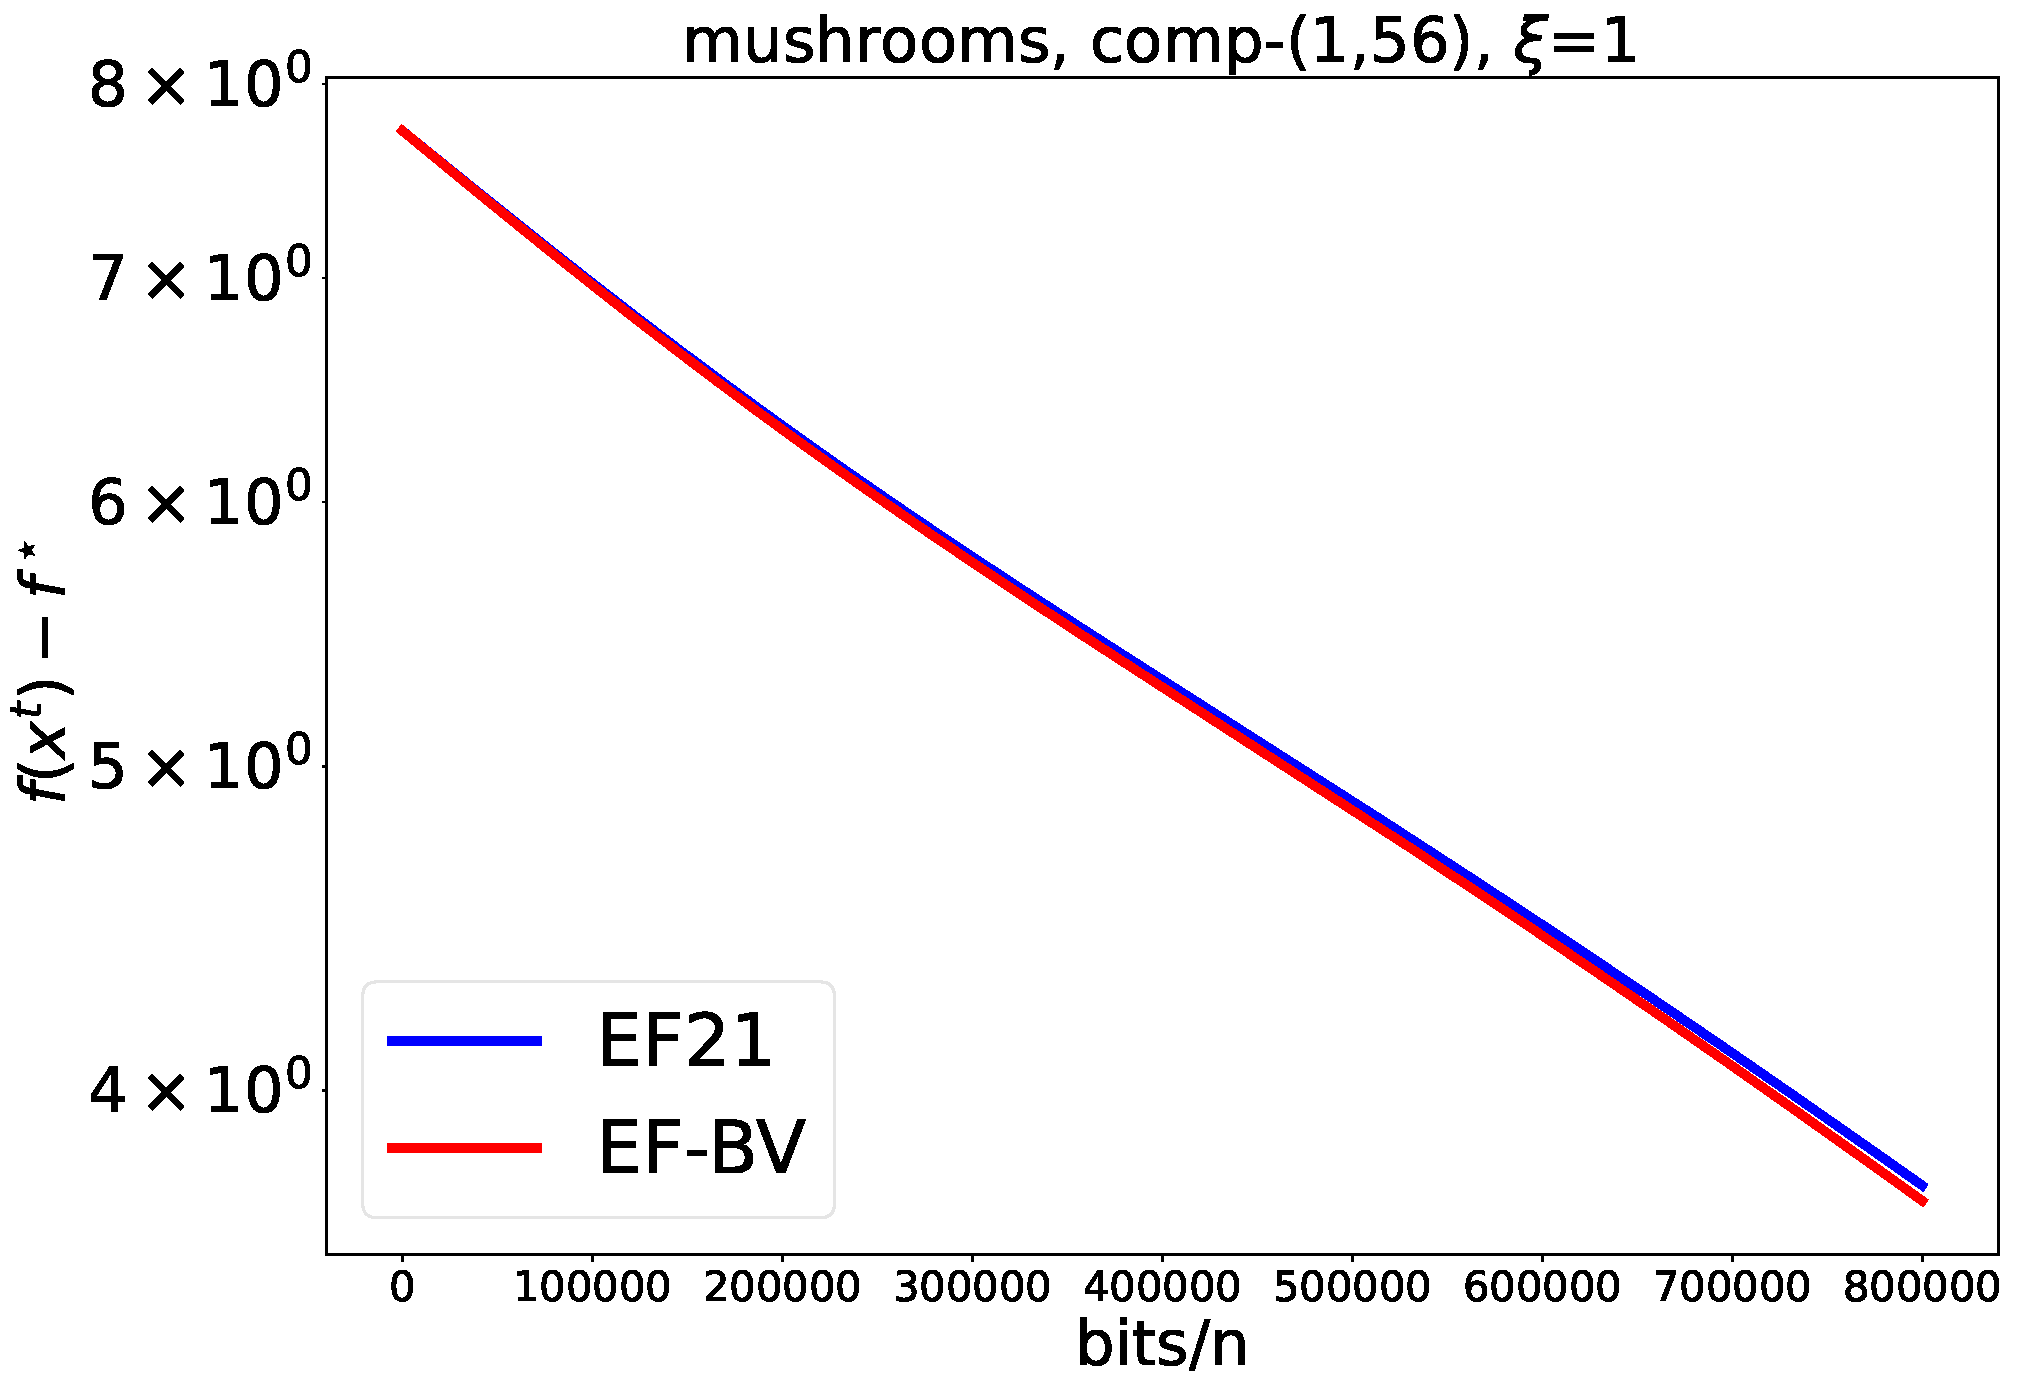
\includegraphics[width=\textwidth]{img/mushrooms/CompK_56_1_mushrooms_8124workers_3000K_20_mushrooms_56_1_1_1_logreg_diff_conv.pdf}
      \end{subfigure}
      \hfill
      \begin{subfigure}[b]{0.48\textwidth}
         \centering
         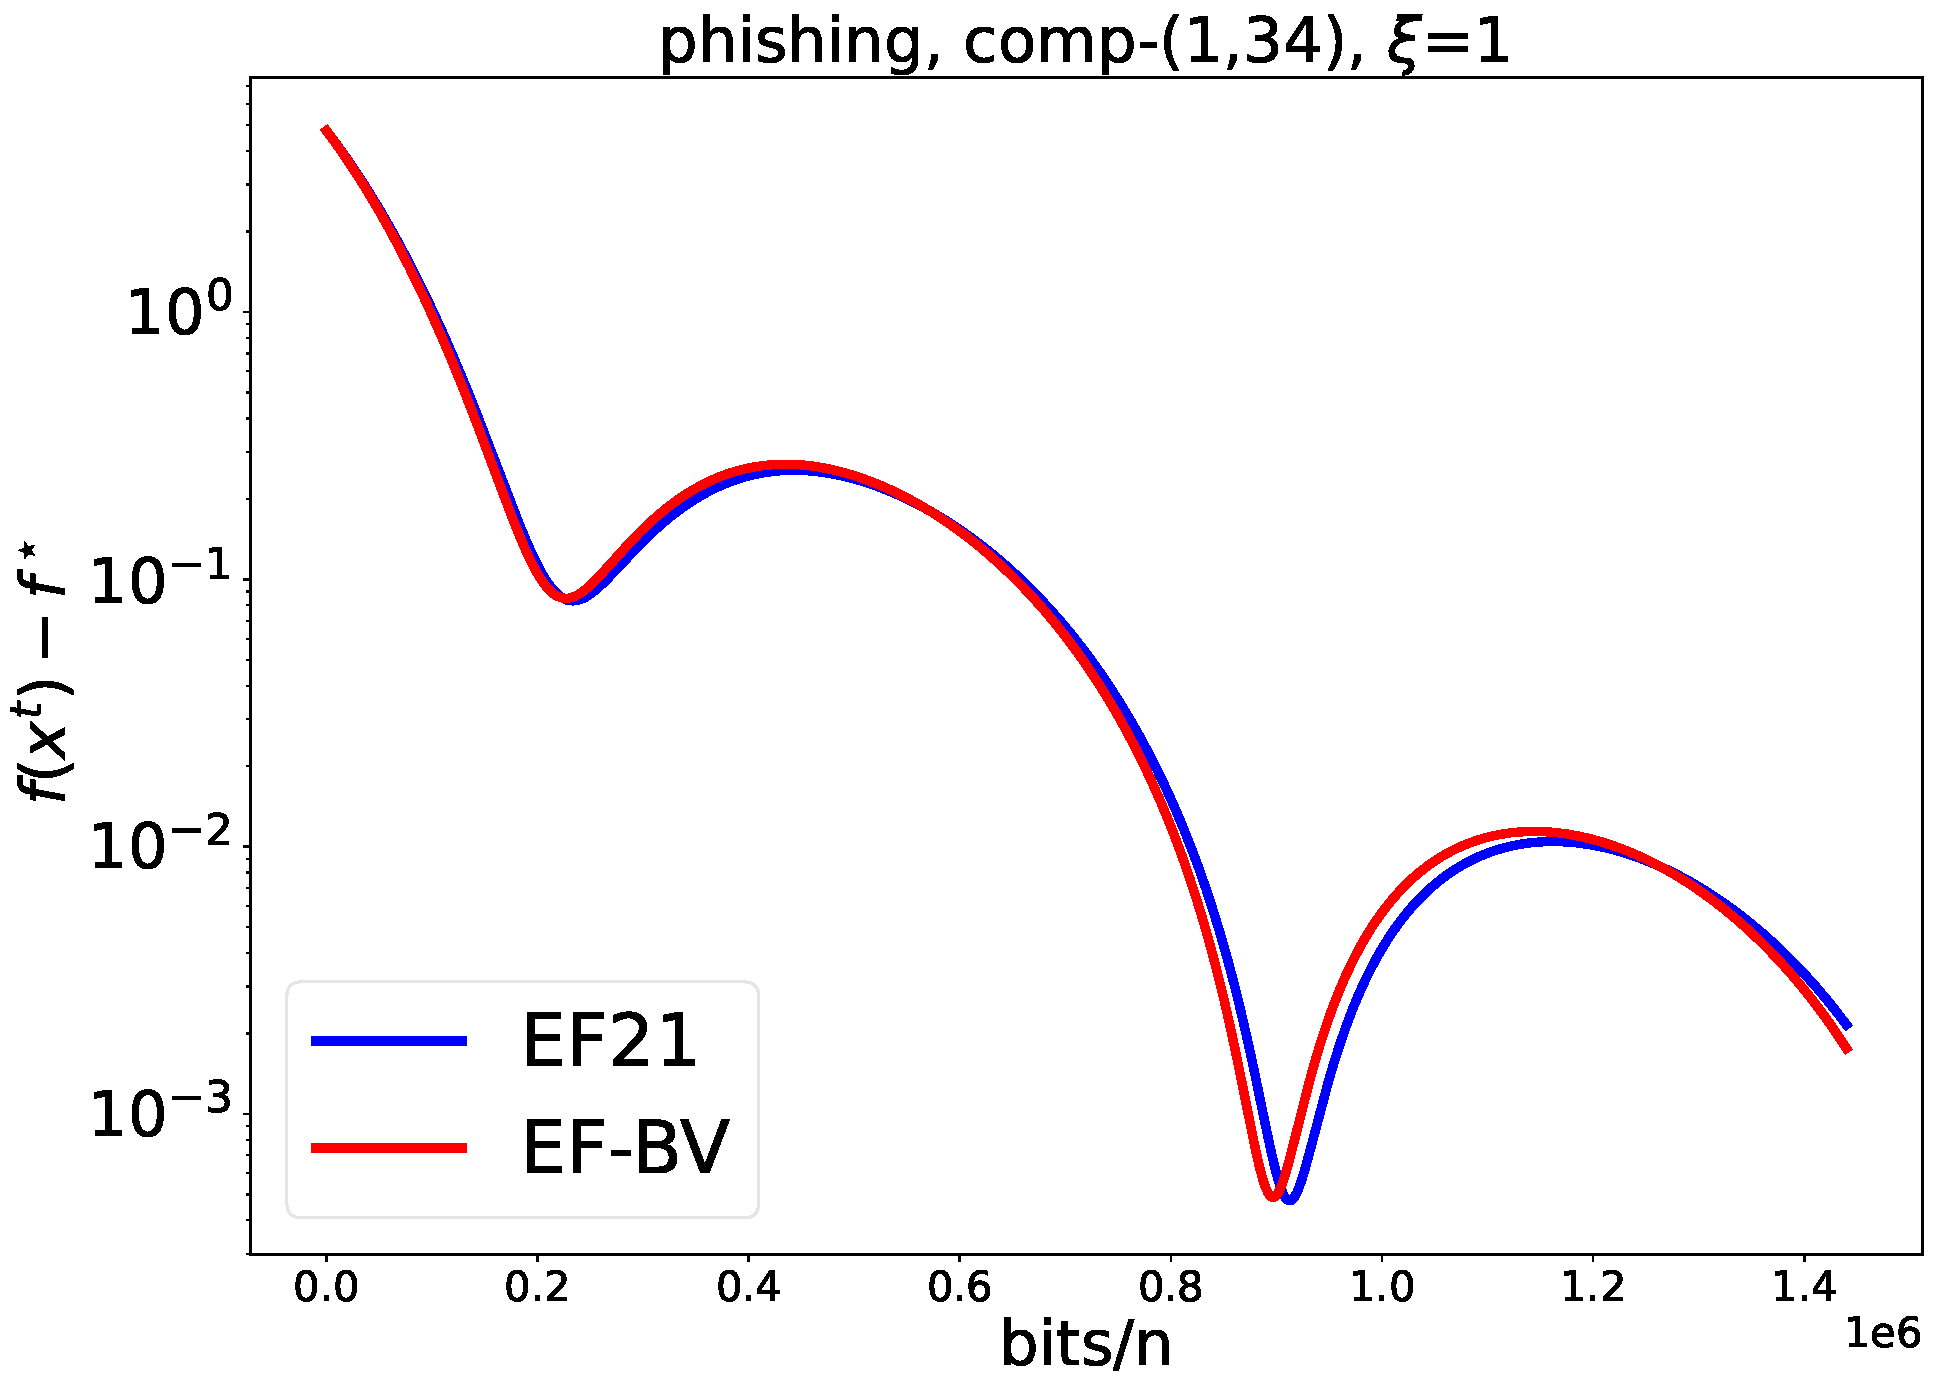
\includegraphics[width=\textwidth]{img/phishing/CompK_34_1_phishing_8124workers_3000K_20_phishing_34_1_1_1_logreg_diff_conv.pdf}
      \end{subfigure}
      \caption{20 workers.}
      \hfill
      \begin{subfigure}[b]{0.48\textwidth}
         \centering
         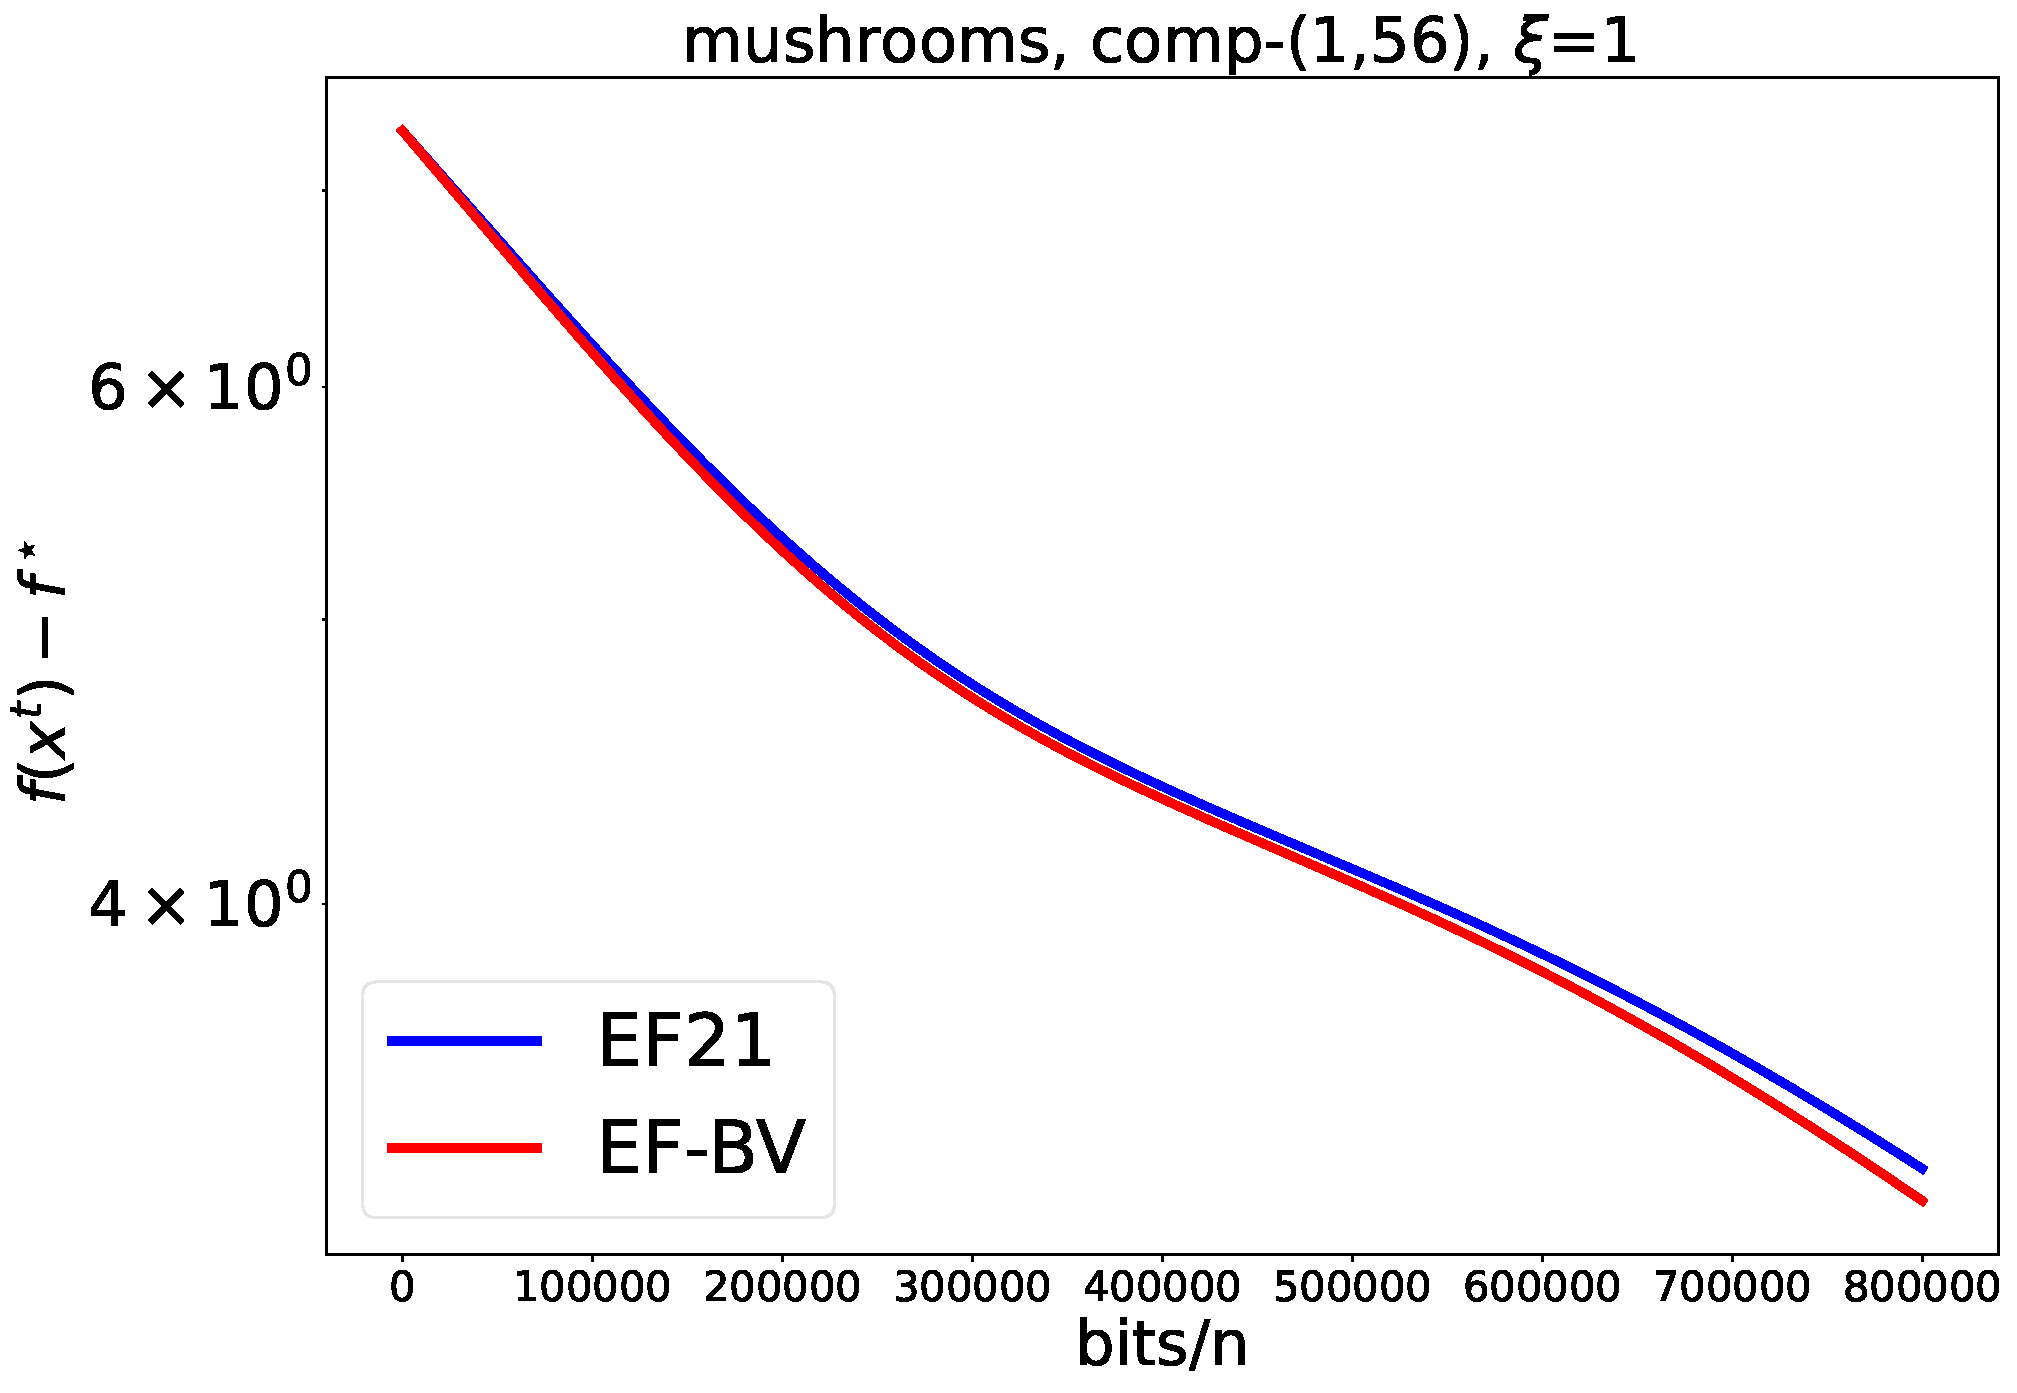
\includegraphics[width=\textwidth]{img/mushrooms/CompK_56_1_mushrooms_8124workers_3000K_50_mushrooms_56_1_1_1_logreg_diff_conv.pdf}
      \end{subfigure}
      \hfill
      \begin{subfigure}[b]{0.48\textwidth}
         \centering
         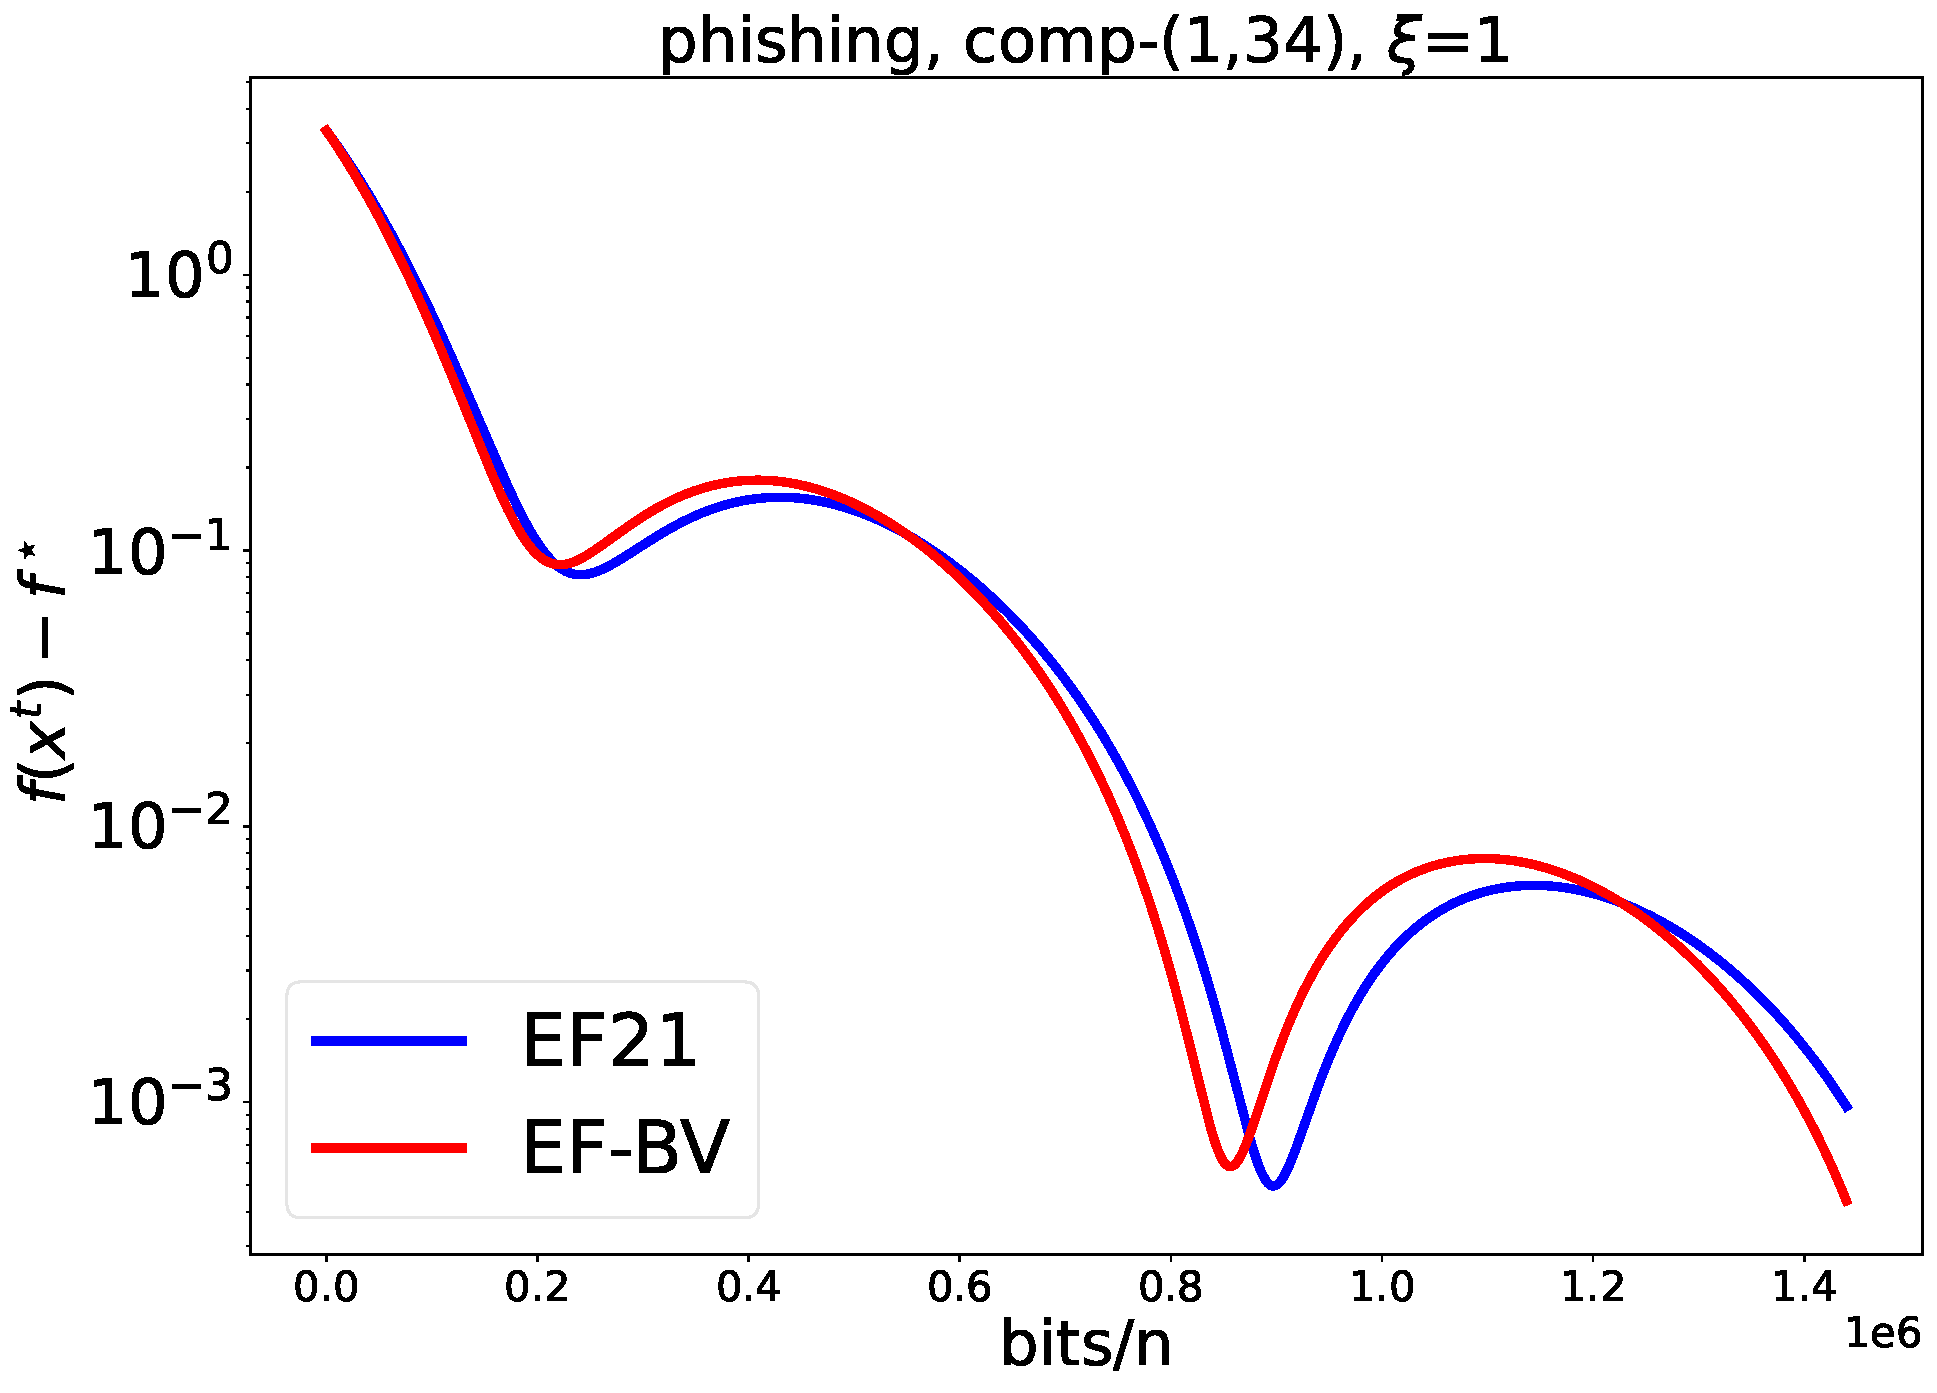
\includegraphics[width=\textwidth]{img/phishing/CompK_34_1_phishing_8124workers_3000K_50_phishing_34_1_1_1_logreg_diff_conv.pdf}
      \end{subfigure}
      \caption{50 workers.}
         \caption{Comparison between \algname{EF21} and \algname{EF-BV} in the convex setting with smaller number of workers. We see the difference between \algname{EF-BV} and \algname{EF21} is smaller, which is align with our theory.}
         \label{12}
   \end{figure}
\end{document}
